\chapter{Results \& Discussion}
\section{Tissue Segmentation}  \label{res_tissue_segm}
Three models were trained to segment the RGB input of H\&E stained image at 20$\times$ magnification
(resolution of 0.5 micron-per-pixel) into three prediction maps:
tumor, stroma, and rest (not white space, but tissue that is neither tumor nor stroma,
for details refer to Table~\ref*{tab:label_data}). The data was separated on the patient
level (or slide level, since there is one slide per patient present)
into training, validation, and test with 80\%, 10\%, and 10\% accordingly.
In order to keep the distribution of the resulting patch numbers (see Table~\ref*{tab:patch_sep})
and dataset sources fair, the patient separation in Table~\ref*{tab:patients_sep} was introduced.

\begin{table}[h!]
    \centering
    \begin{tabular}{ l c c c }
        \hline
        & Train & Validation & Test \\
        \hline
        TCGA-BRCA & 120 & 16 & 15 \\
        RUMC & 20 & 3 & 3 \\
        JB & 16 & 1 & 1 \\
        \hline
        & 156 & 20 & 19 \\
    \end{tabular}
\caption{\label{tab:patients_sep} Split of patients across different medical sources
into train, validation, and test sets for segmentation tasks.}
\end{table}

The patches were created using a sliding window approach with 256$\times$256 sized patches
and stride equals 128. The additional rotation augmentation was applied, by rotating each patch
5 times at 9 degrees each.

\begin{table}[h!]
    \centering
    \begin{tabular}{ l c c c c c c c c c}
        \hline
        & \multirow{2}{*}{slides} & \multirow{2}{*}{ROIs}& \multirow{2}{*}{patches}& \multicolumn{6}{c}{Number of patches that include}\\ 
        \cline{5-10}
        & & & & Tumor & Stroma & Rest & 1 class & 2 classes & 3 classes\\
        \hline
        Train & 156 & 228 & 220\,567 & 154\,734 & 172\,046 & 107\,506 & 63\,919 & 99\,577 & 57\,071 \\
         &  &  &  & (70\%) & (78\%) & (49\%) & (29\%) & (45\%) & (26\%) \\
        Valida- & 20 & 25 & 29\,465 & 16\,884 & 22\,187 & 13\,954 & 11\,171 & 13\,028 & 5\,266 \\
        tion &  &  &  & (57\%) & (75\%) & (47\%) & (38\%) & (44\%) & (18\%)\\
        Test & 19 & 33 & 30\,248 & 18\,194 & 25\,630 & 14\,787 & 8\,548 & 15\,037 & 6\,663\\
         &  &  &  & (60\%) & (85\%) & (49\%) & (28\%) & (50\%) & (22\%)\\
        \hline
        & 195 & 286 & 280\,280 &  &  &  & & & \\
    \end{tabular}
    \caption{\label{tab:patch_sep} Overview of patches that were split into train, validation,
    and test sets for tissue segmentation. The percentages indicate the fraction of a specific conditioned group of patches to the number of all patches in the "patches" column.}
\end{table}

The models were trained with the mmsegmentation toolbox~\cite{mmseg2020}. 
All models were trained for 160K iterations with Cross Entropy Loss and
standard data augmentation techniques including resizing at a random sample scale in the range
of (0.5, 2.0), cropping with the maximum 0.75 of a single category present, flipping with 0.5 probability,
and application of photometric distortion which includes 0.5 probability for each of the following transformations: random brightness, contrast, saturation, hue and color adjustments. 
The DeepLabv3+ model was taken as a baseline and trained with ResNet50 backbone,
Adam optimizer, learning rate equals 0.0001 and batch size of 64. Whereas the
transformer-based SegFormer-B5 (further referred to as SegFormer) architecture was trained once with the same setup of
Adam optimizer, 0.0001 learning rate and batch size of 64, and additionally, as 
in original paper~\cite*{xie2021segformer}, using AdamW optimizer, the learning rate
set to an initial value of 0.00006 and then used a poly learning rate schedule with
factor 1.0 by default.

\begin{table}[h!]
    \centering
    \begin{tabular}{ l c c c c c c c c}
        \hline
        \multirow{2}{*}{Model} & \multirow{2}{*}{FLOPs} & \multirow{2}{*}{Params} & \multirow{2}{*}{Iterations} & \multirow{2}{*}{Runtime} & \multicolumn{4}{c}{mDice}\\
        & & & & & Overall & Tumor & Stroma & Rest \\
        \hline
        DeepLabv3+ & 44.16 & 43.58 M & 160 K & 1d 12h 2m & \textbf{85.25} & 85.13 & 88.07 & 83.66\\
        SegFormer & 12.96 & 81.97 M & 160 K  & 3d 4h 30m & 83.44 & 83.83 & 86.32 & 80.16\\
        SegFormer, & \multirow{2}{*}{12.96} & \multirow{2}{*}{81.97 M} & \multirow{2}{*}{160 K} & \multirow{2}{*}{3d 4h 25m} & \multirow{2}{*}{84.93} & \multirow{2}{*}{85.40} & \multirow{2}{*}{87.40} & \multirow{2}{*}{82.00}\\
        AdamW & & & & & & & & \\
        \hline
    \end{tabular}
\caption{\label{tab:tissue_perform} Overview of the trained tissue segmentation models. The runtime is given for a training on one GPU NVIDIA A100 SXM4.}
\end{table}

\begin{figure}[H]
    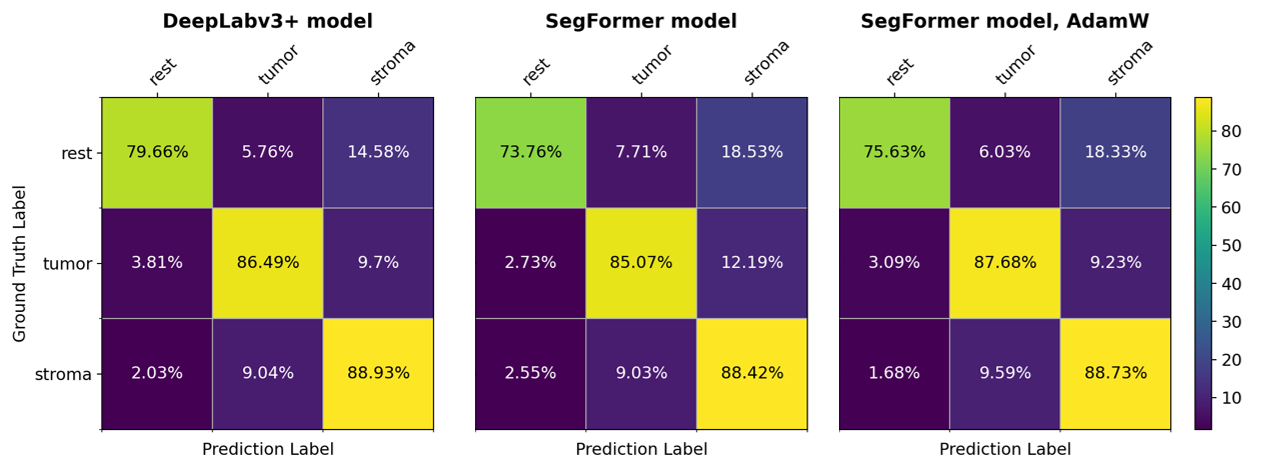
\includegraphics[width=\linewidth]{figures/tissue/conf_matrices.png}
    \caption{Confusion matrices on pixel level for DeepLabv3+, SegFormer and SegFormer with AdamW optimizer
    based on test set of 32 ROIs.}
    \label{fig:tissue_confusion}
\end{figure}

During a close investigation of test data, one slide (with the prefix TCGA-OL-A5RW-01Z-00-DX1)
was excluded from the test set due to an obvious image-mask mismatch. The overall
performance of the models, the number of parameters, and the resulting dice score after testing on 
32 test images can be found in Table~\ref*{tab:tissue_perform}. The first thing that catches the eye is the severe runtime difference of
SegFormer-based methods compared to the DeepLabv3+ accompanied by doubled number of parameters.
None of the SegFormer approaches outperform the DeepLabv3+, but the performance
is comparable, which can be also observed in the confusion matrices in Figure~\ref*{fig:tissue_confusion}.
Both SegFormer-based methods show difficulty correctly segmenting rest regions, whereas
SegFormer AdamW slightly outperforms DeepLabv3+ in the number of true positive detected tumor pixels.

As previously mentioned, the dataset originates from three medical
institutions which make it reasonable to characterize the performance separately.
The boxplots in Figure~\ref*{fig:tissue_dice_boxplots} indicate that the performance of
the DeepLabv3+ and SegFormer AdamW models in TCGA-BRCA and JB groups are fairly invariant.
Whereas the RUMC group accounts not only for the lower performance of SegFormer-based methods
in segmenting rest regions but also for an improvement of tumor region segmentation by SegFormer AdamW
model both observed in Figure~\ref*{fig:tissue_confusion}.

\begin{figure}[H]
    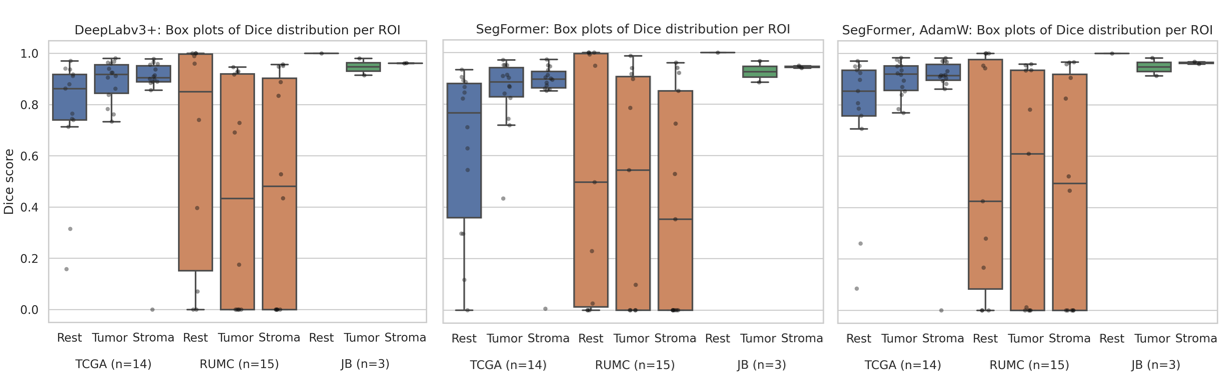
\includegraphics[width=\linewidth]{figures/tissue/dices.png}
    \caption{Boxplots of pixel wise calculated dice score across three datastes (TCGA-BRCA, RUMC, JB) and three segmentation labels.}
    \label{fig:tissue_dice_boxplots}
\end{figure} 

The additional specialty that Figure~\ref*{fig:tissue_dice_boxplots} brings to light is
the considerable number of RUMC ROIs that have been evaluated with dice scores close to
zero across all models. Due to the nature of the Dice score, those can be originated from
significant numbers of either false positives, false negatives, or both.
According to the boxplots of precision and recall in Figure~\ref*{fig:tissue_pr_r_boxplots}
the precision across all models has more close zero values that indicate more frequent
false positives. 
There are clear examples, such as Figure~\ref*{fig:TC_S01_P000159},
where the ground truth includes exclusively rest but all trained models provide multiple class predicitons.
Even though there are also opposite examples of regions that were solely annotated as rest and predicted as
such (which then lead to occasional dice, precision, and recall equal to one, see Figure~\ref*{fig:tissue_dice_boxplots}
and~\ref*{fig:tissue_pr_r_boxplots}), the issue of false positives needed to be further explored.

Out of the original 81 RUMC ROIs, 14\% of ROIs carry the annotation of only class label 7 - rest.
According to the organizers, that class contains regions of several tissue compartments that are not
specifically annotated in the other categories, such as healthy stroma, erythrocytes, adipose tissue,
skin, nipple, etc. There are none of such annotations in TCGA-BRCA or JB datasets.
After forming new masks with only three classes, the number of RUMC ROIs annotated completely as rest grew
to 17\% due to an additional ROI that represented only necrosis not in-situ.
Even though the number of all-rest-ROIs in the new TCGA-BRCA is 0.2\% and even 22\% in JB, RUMC ROIs
originally annotated as rest (label 7) need to be minded.
Those ROIs may not be the consequence of a bad annotation, but in future experiments,
it should be addressed by assigning them a reduced sampling rate, lower weights or excluding those completely. 

The patch size and the sampling stride define the overlap between consecutively extracted
patches from the WSI or ROI image. The stitching of the segmented patches introduced tiling artifacts
visible in Figure~\ref*{fig:TC_S01_P000159} and~\ref*{fig:TCGA-GM-A2DF}.
Since DeepLabv3+ and transformer based networks showcase it, the reason might be an
overfitting problem due to small patches of 256$\times$256 and 50\% overlap used for training and validation.
Hence the problem can be tackled by
applying less spacing during patch formation and additional augmentations.
During inference, Khened, M et al.~\cite*{khened2021generalized} addressed a similar
problem by increasing patch size by a factor of 4 (from 256$\times$256 to 1024$\times$1024)
and keeping 50\% overlap. Due to time constraints and difficulties in migrating transformer based
models to accept generalized input, this experiment was not further pursued.

A close look at the prediction also revealed that at some cases dice scores might suffer due to some inaccuracies
in the annotations. Figure~\ref*{fig:TCGA-GM-A2DF} showcases that all models were
penalized for detecting a rest region inside of the tumor, which was probably learned
with some dependency to the presence of white space, which also present in the same slide
(the bubles in the lower part of the image) and was annotated as rest.

Nonetheless, there are positive segmentation results present, such as JB ROIs depicted in
Figure~\ref*{fig:s_250B_1} and~\ref*{fig:s_250B_2} where the performance of SegFormer AdamW
is either very close or slightly better then DeepLabv3+. 
Curiously, in Figure~\ref*{fig:s_250B_2} the SegFromer AdamW performs slightly better partly
because this model, in contrast to the rest, did not attempt to annotate the small possibly
tumorous region in the upper left corner (around (250, 200), which is not annotated in ground
truth but visually highly similar to the tumor regions in this example). To decide whether
this is an encouraging behavior the pathologist must be consulted, but in some cases,
SegFromer AdamW manages to considerably outperform DeepLabv3+, as visualized in
Figure~\ref*{fig:TCGA-EW-A1P4}.

For tissue segmentation, the TiGER challenge evaluated the Dice score for stroma,
i.e. Tumor-associated stroma grouped with inflamed stroma versus all other classes
and invasive tumor against all other classes (see Table~\ref{tab:label_data}). 
The motivation for such a metric is that regions of invasive tumors and 
tumor-associated stroma play a central role in the definition of the TILs score.
The resulting values are registered in Table~\ref{tab:tissue_compare}. 
The final TiGER best result was achieved by a segmentation model that used
UperNet~\cite{xiao2018unified} with visual attention network~\cite{guo2022visual}
as the backbone, hence there are some parallels to both of the trained models:
use of hierarchical representation and attention.
Due to different class definitions (current tumor class includes extra in-situ tumor,
see Table~\ref{tab:label_data}) and the TiGER results are based on an experimental
set of 26 WSIs and a final test of 38 WSIs, hence different amounts and sources of
test data, the results in Table~\ref{tab:tissue_compare} can not be compared.
It prohibits making the statement that trained models in this work outperform the models
developed within the TiGER challenge, but their results make them promising for
further experiments to acquire real comparison.

\begin{table}[h!]
    \centering
    \begin{tabular}{ l c c c c c c }
        \hline
         & \multirow{2}{*}{DeepLabv3+} & \multirow{2}{*}{SegFormer} & SegFormer, & & TiGER best & TiGER best\\
         &  &  & AdamW & & (experimental) & (final)\\
        \hline
        Dice score & 0.866 & 0.851 & 0.864 & & 0.794 & 0.812 \\
        \hline
    \end{tabular}
\caption{\label{tab:tissue_compare} Dice score for stroma compared between the TiGER challenge leaderboard
results versus three models developed in this work. The results were obtained from different data.}
\end{table}

The observation of similar performance between the developed methods complies with the literature. 
As Dosovitskiy, A et al.~\cite*{dosovitskiy2020image} witnessed, transformer based models yield
modest accuracies of a few percentage points below ResNets of comparable size. It is claimed
that this outcome is expected, since Transformers lack some of the inductive biases
inherent to CNNs, such as translation equivariance and locality, and therefore do not generalize
well when trained on insufficient amounts of data. Liu, Y at al.~\cite{liu2021efficient} came to
a similar conclusion and showed that the performance of visual transformers largely varies when
trained with small and medium datasets. A typical fine-tuning scenario that results in major
improvements in the performance is pre-training the model on a big dataset (e.g., ImageNet) which
is also done in SegFromer paper~\cite*{xie2021segformer} and repeated strong data augmentations~\cite{touvron2021training}.
An alternative is the use of a principled optimizer to avoid excessive demands of data,
computing, and hyperparameters tuning~\cite*{chen2021vision}.The importance of the optimizer
choice is also seen in the presented experiments of SegFromer with Adam and AdamW optimizers.
Adam and AdamW were selected according to literature reporting that these adaptive gradient
methods do not underperform momentum or gradient descent optimisers~\cite{choi2019empirical}.
The evidence that AdamW is a better choice, agrees with the prior works that use AdamW to
optimize ViT models from random initialization~\cite{xiao2021early}. Generally using AdamW
to optimize deep transformers is extensively practiced in the community~\cite{anonymous2023applying},
posiibly because AdamW yields models that generalize better.

Due to time constraints, there were no further experiments to improve the performance of transformer
based models, which could involve the previously noticed pre-training on ImageNet, increasing
the number of argumentations, or applying different optimizers.
Hence, while the SegFormer AdamW model remains promising, due to overall better performance and
runtime, this thesis will use the DeepLabv3+ model for further inferences and analysis.
For model inference, the model with the best pixel-wise Dice score on the validation set was used.
Patches of size 256$×\times$256 were extracted from the tissue region at 20$\times$ magnification
with a stride of 184 (for faster runtime). The whitespace was extracted by using thresholding and
inference of non-background pixels was then performed.

\begin{figure}[H]
    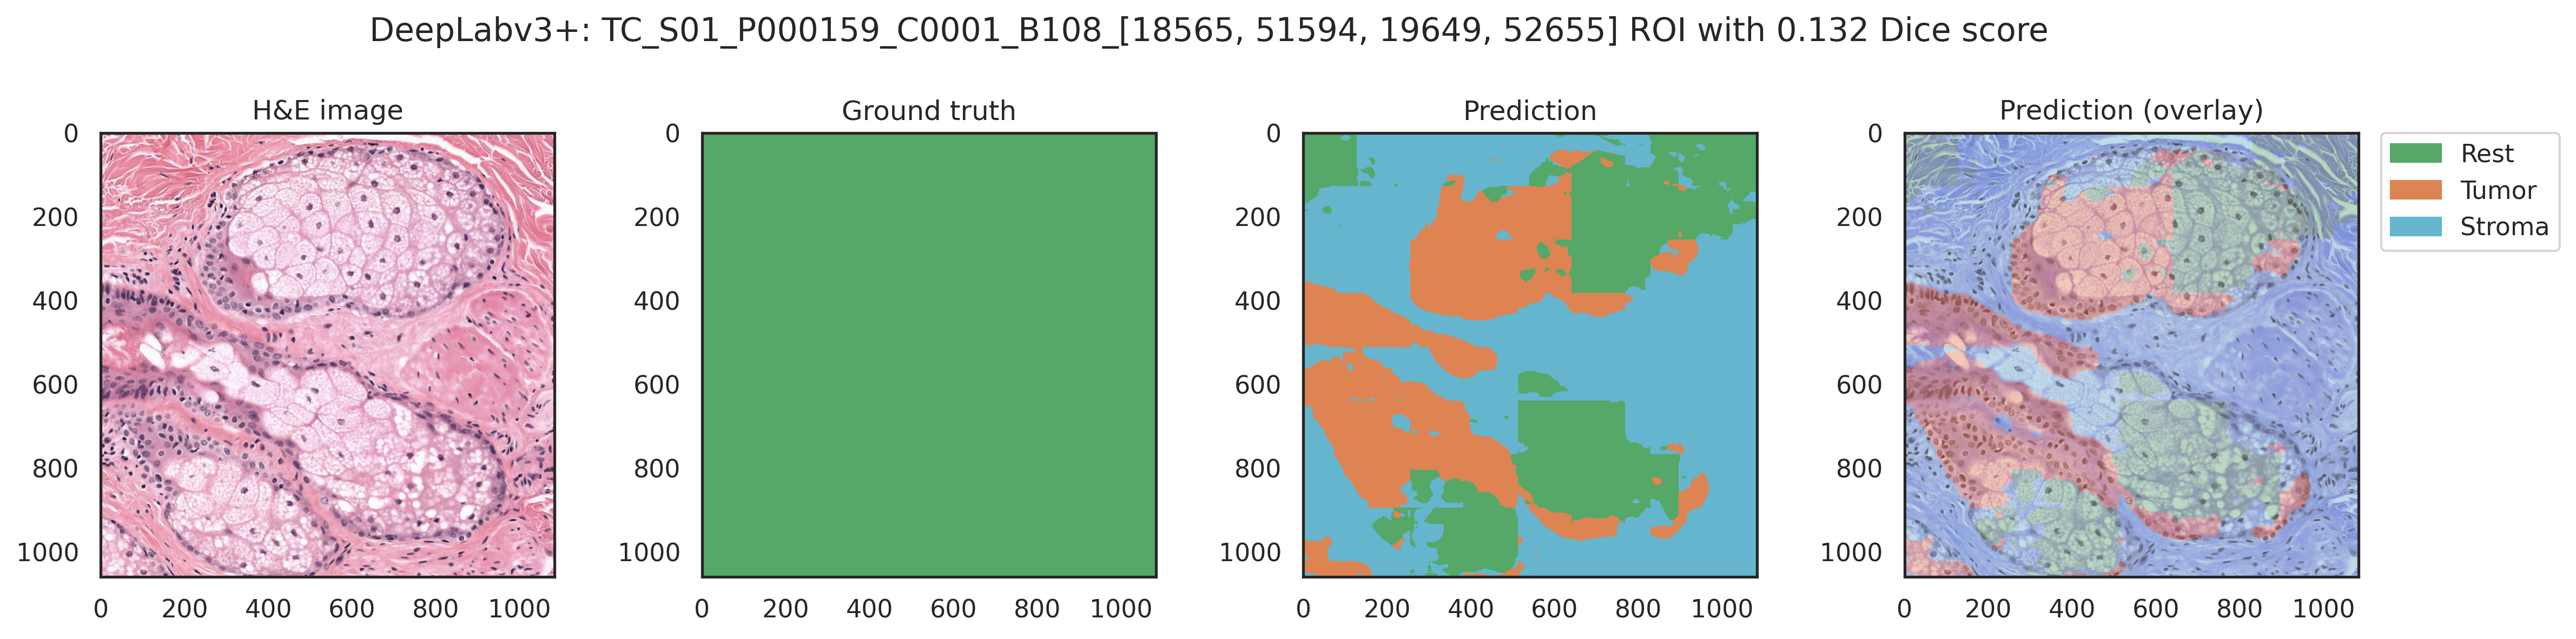
\includegraphics[width=\linewidth]{figures/tissue/deeplabv3+_dice_tc_TC_S01_P000159_C0001_B108_[18565,_51594,_19649,_52655]_check.png}
    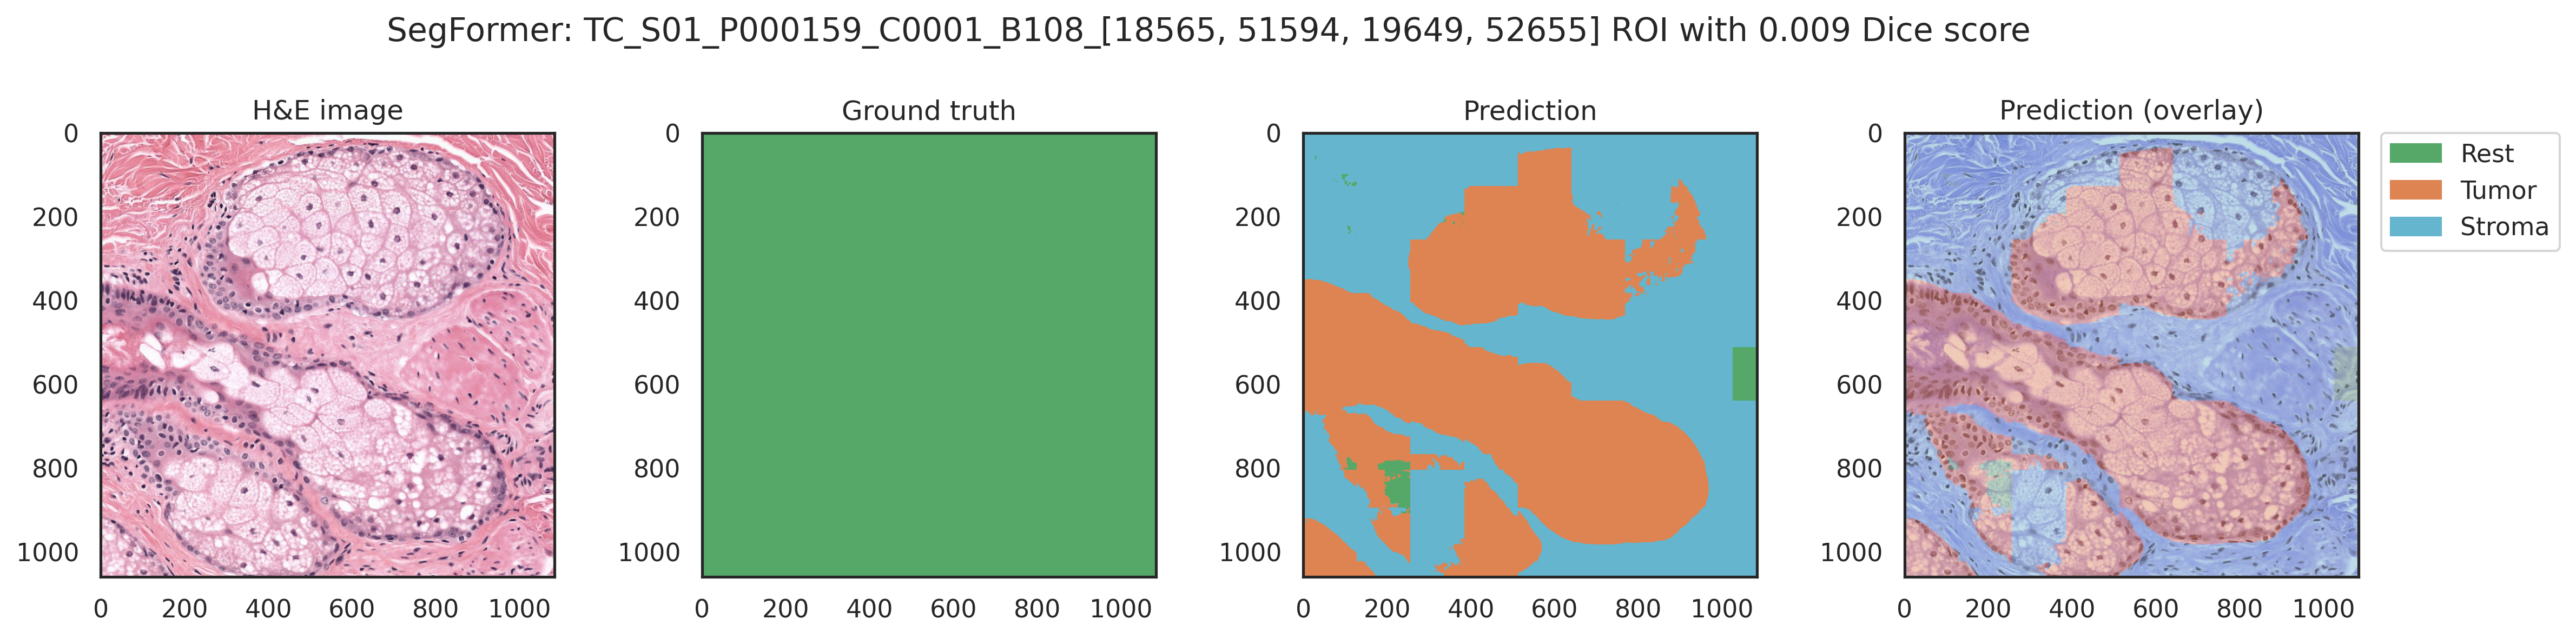
\includegraphics[width=\linewidth]{figures/tissue/segformer_dice_tc_TC_S01_P000159_C0001_B108_[18565,_51594,_19649,_52655]_check.png}
    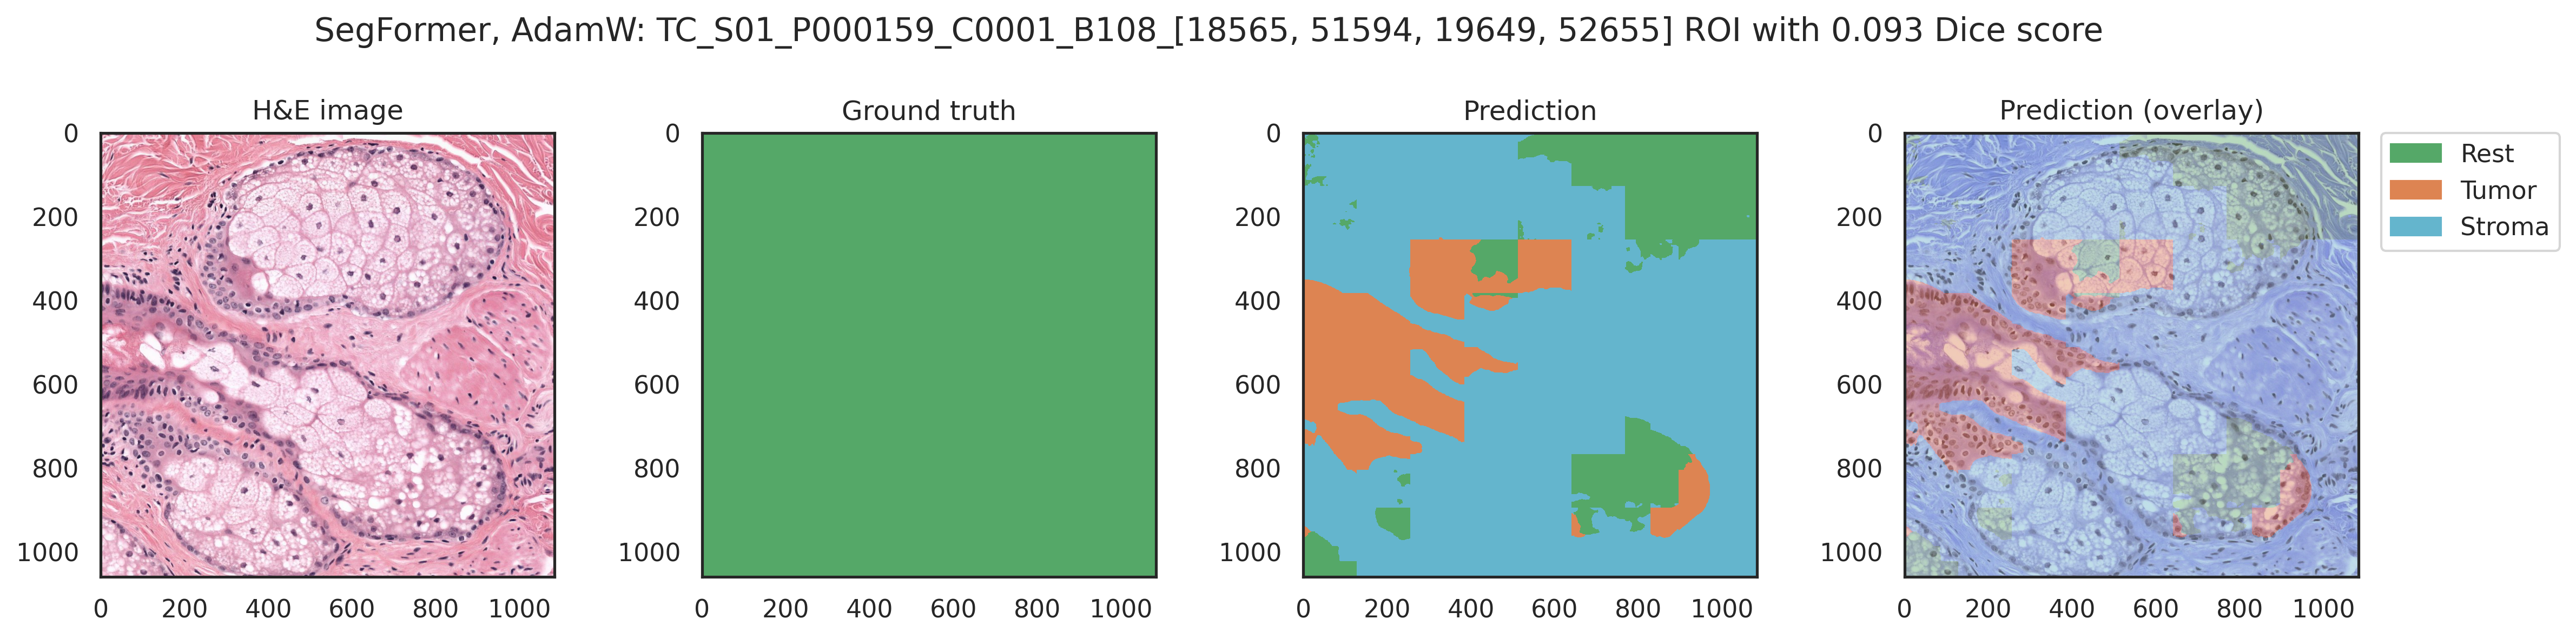
\includegraphics[width=\linewidth]{figures/tissue/segformer,_adamw_dice_tc_TC_S01_P000159_C0001_B108_[18565,_51594,_19649,_52655]_check.png}
    \caption{Example of rich false positive segmentation RUMC ROI that contributes to the cases of close zero dice scores.}
    \label{fig:TC_S01_P000159}
\end{figure}

\begin{figure}[H]
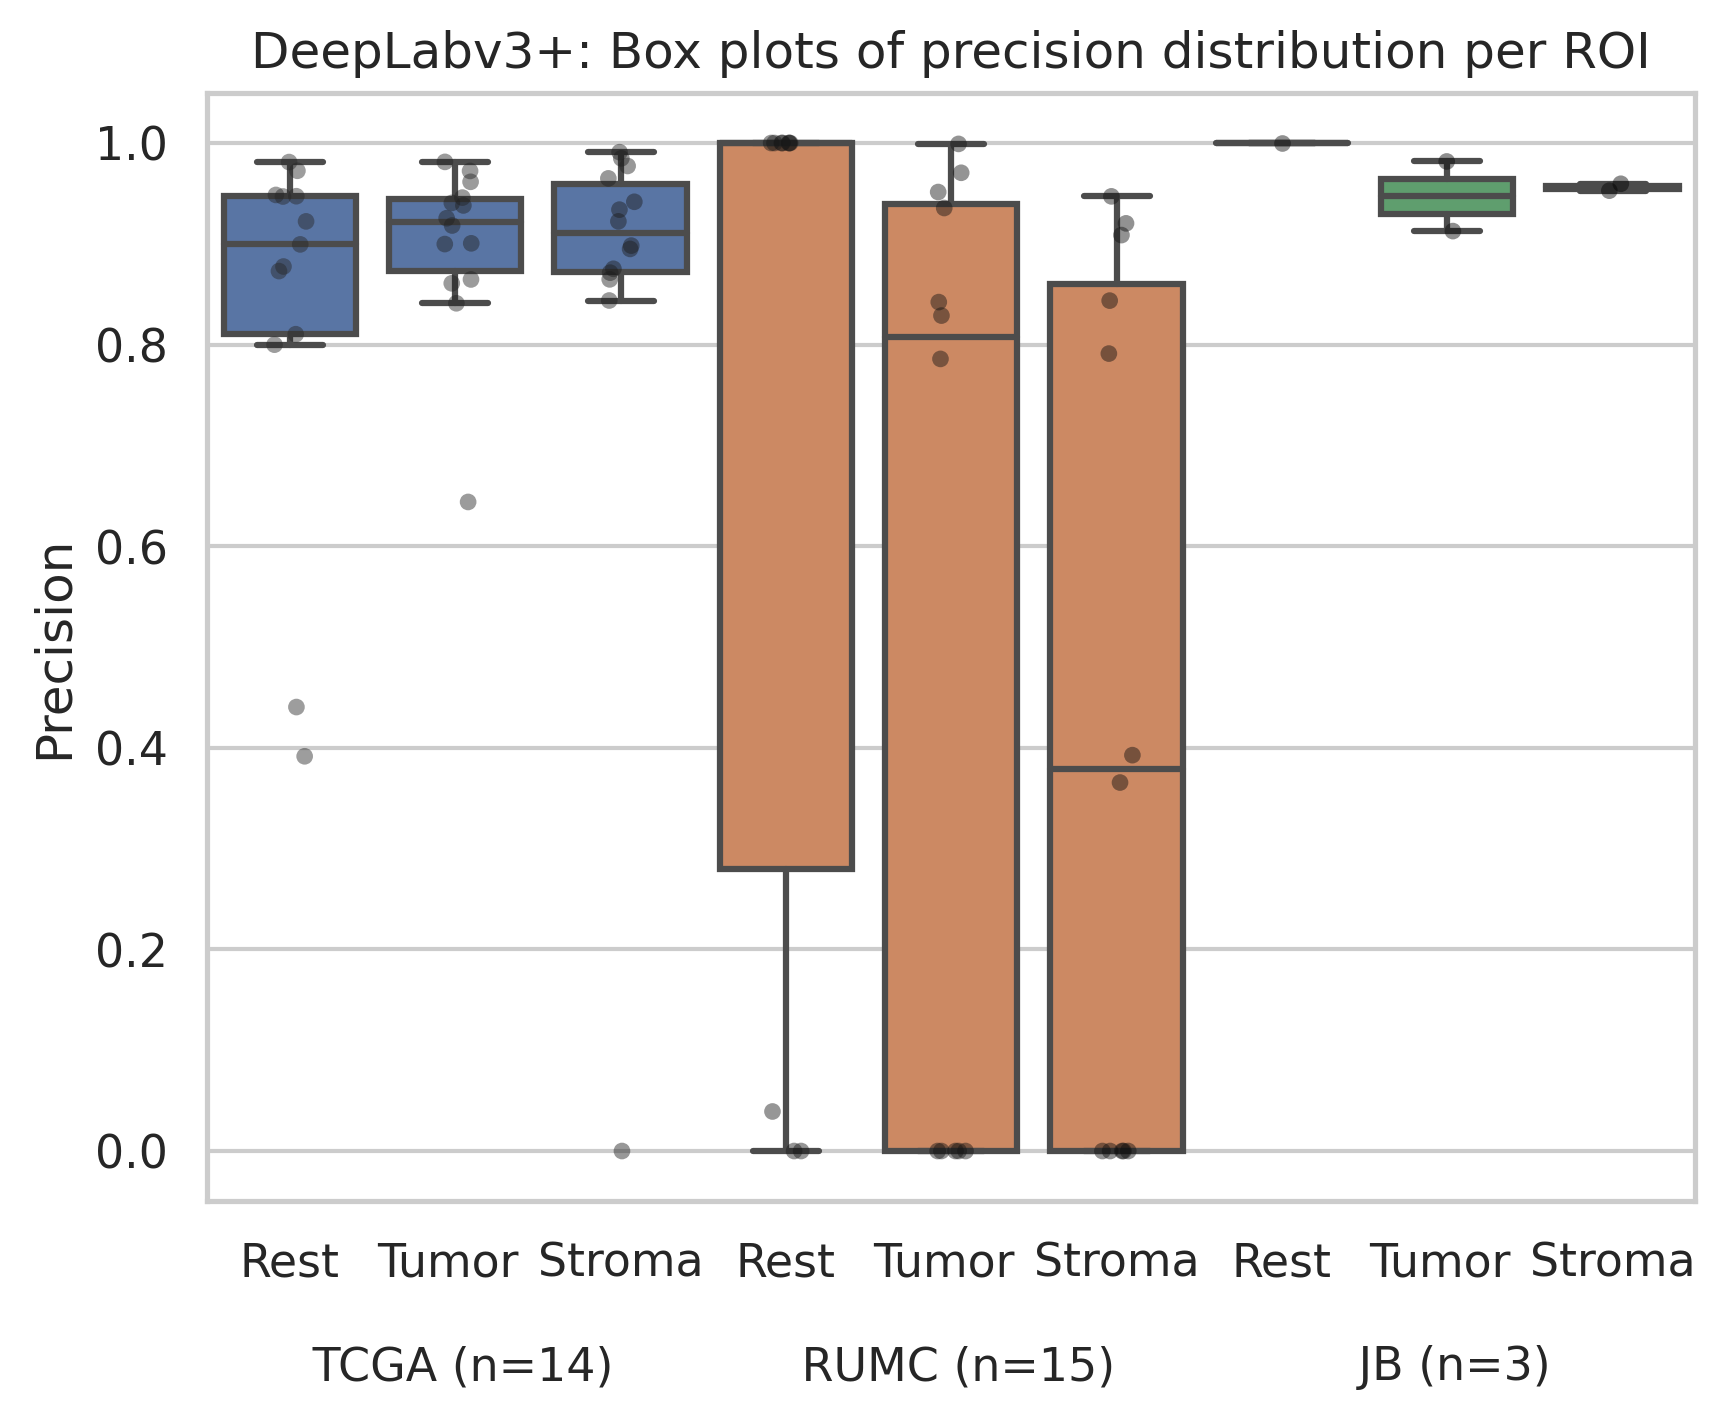
\includegraphics[width=.5\linewidth]{figures/tissue/deeplabv3+_prec_roi_wsirois.png}
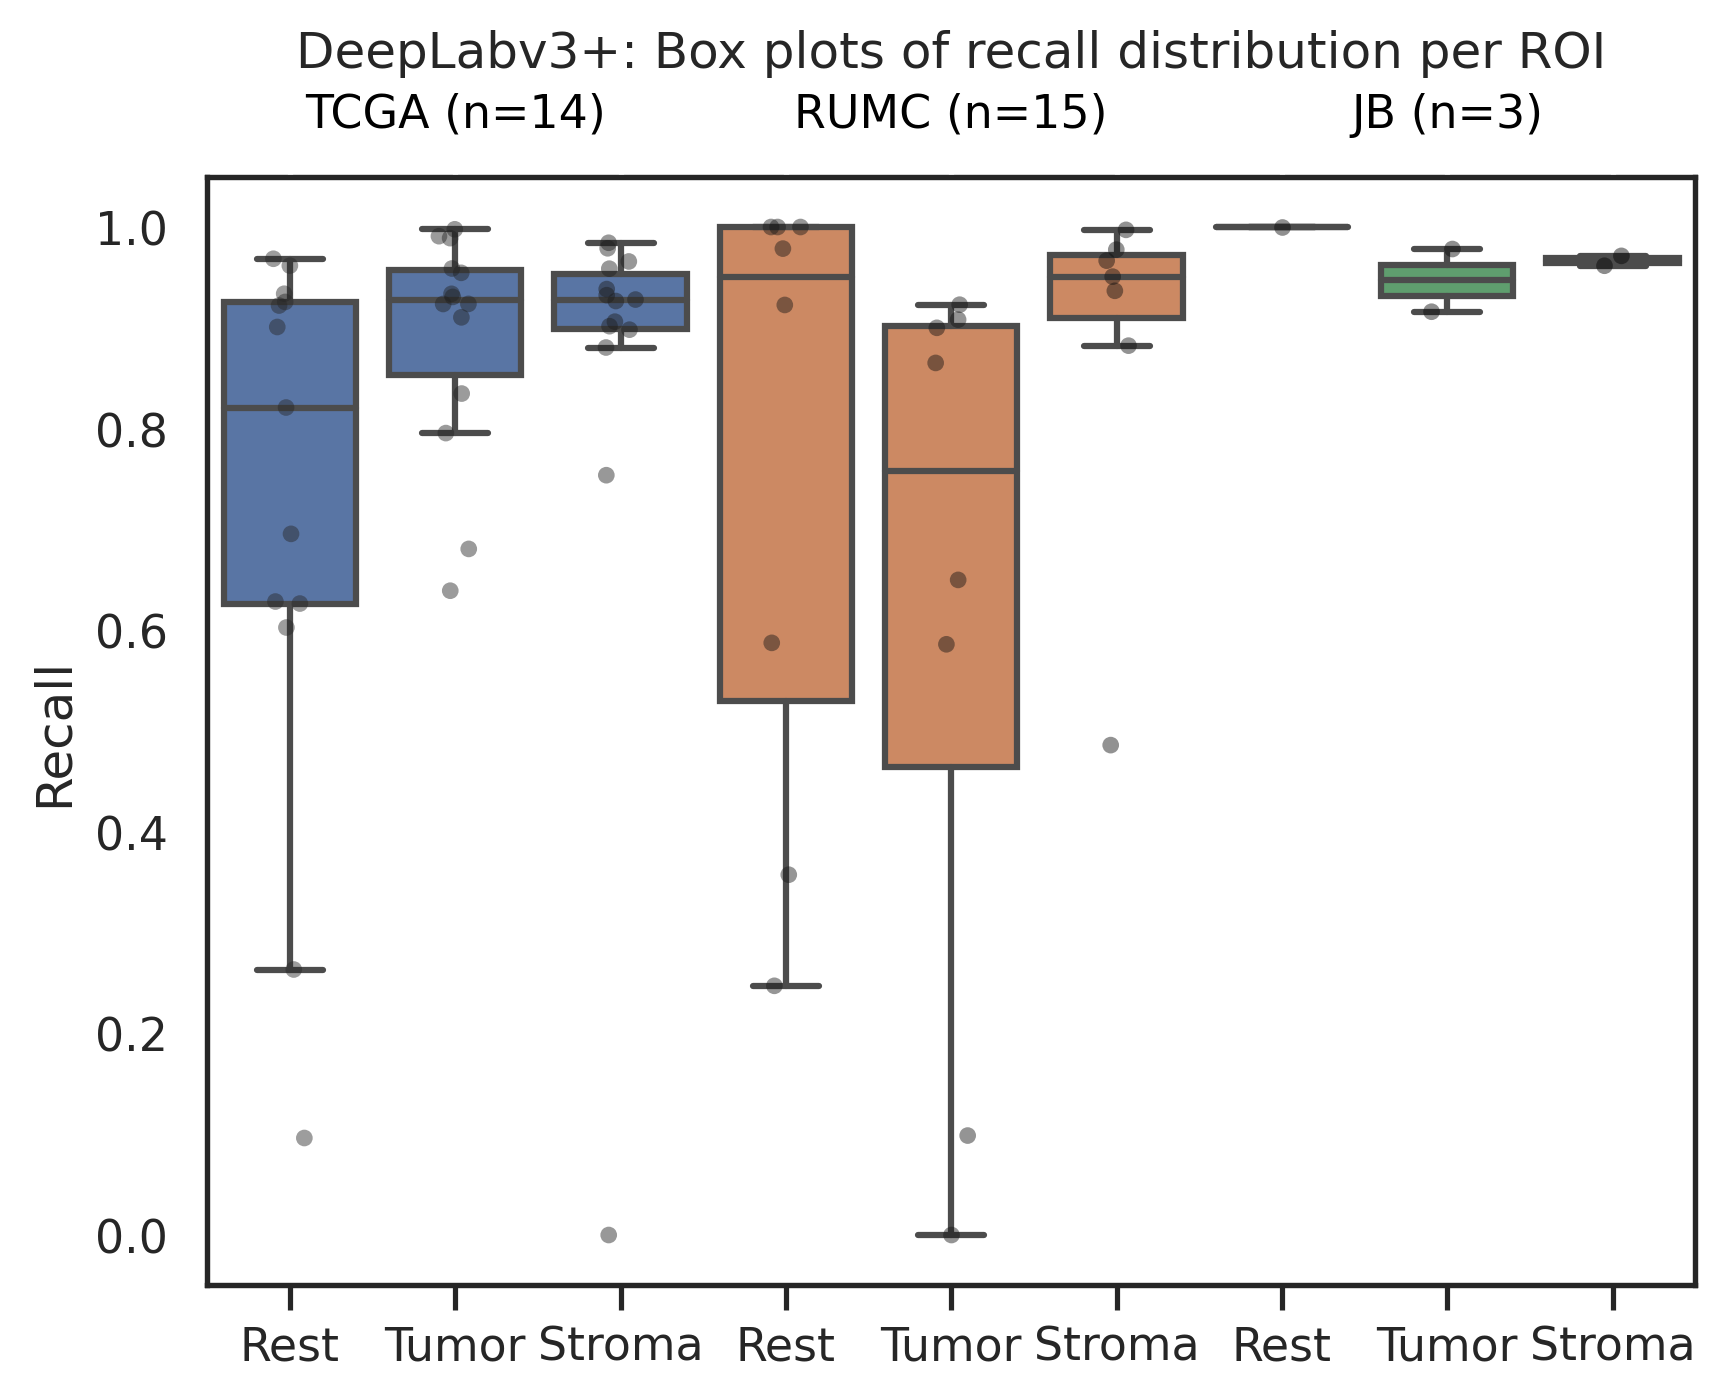
\includegraphics[width=.5\linewidth]{figures/tissue/deeplabv3+_recall_roi_wsirois.png}

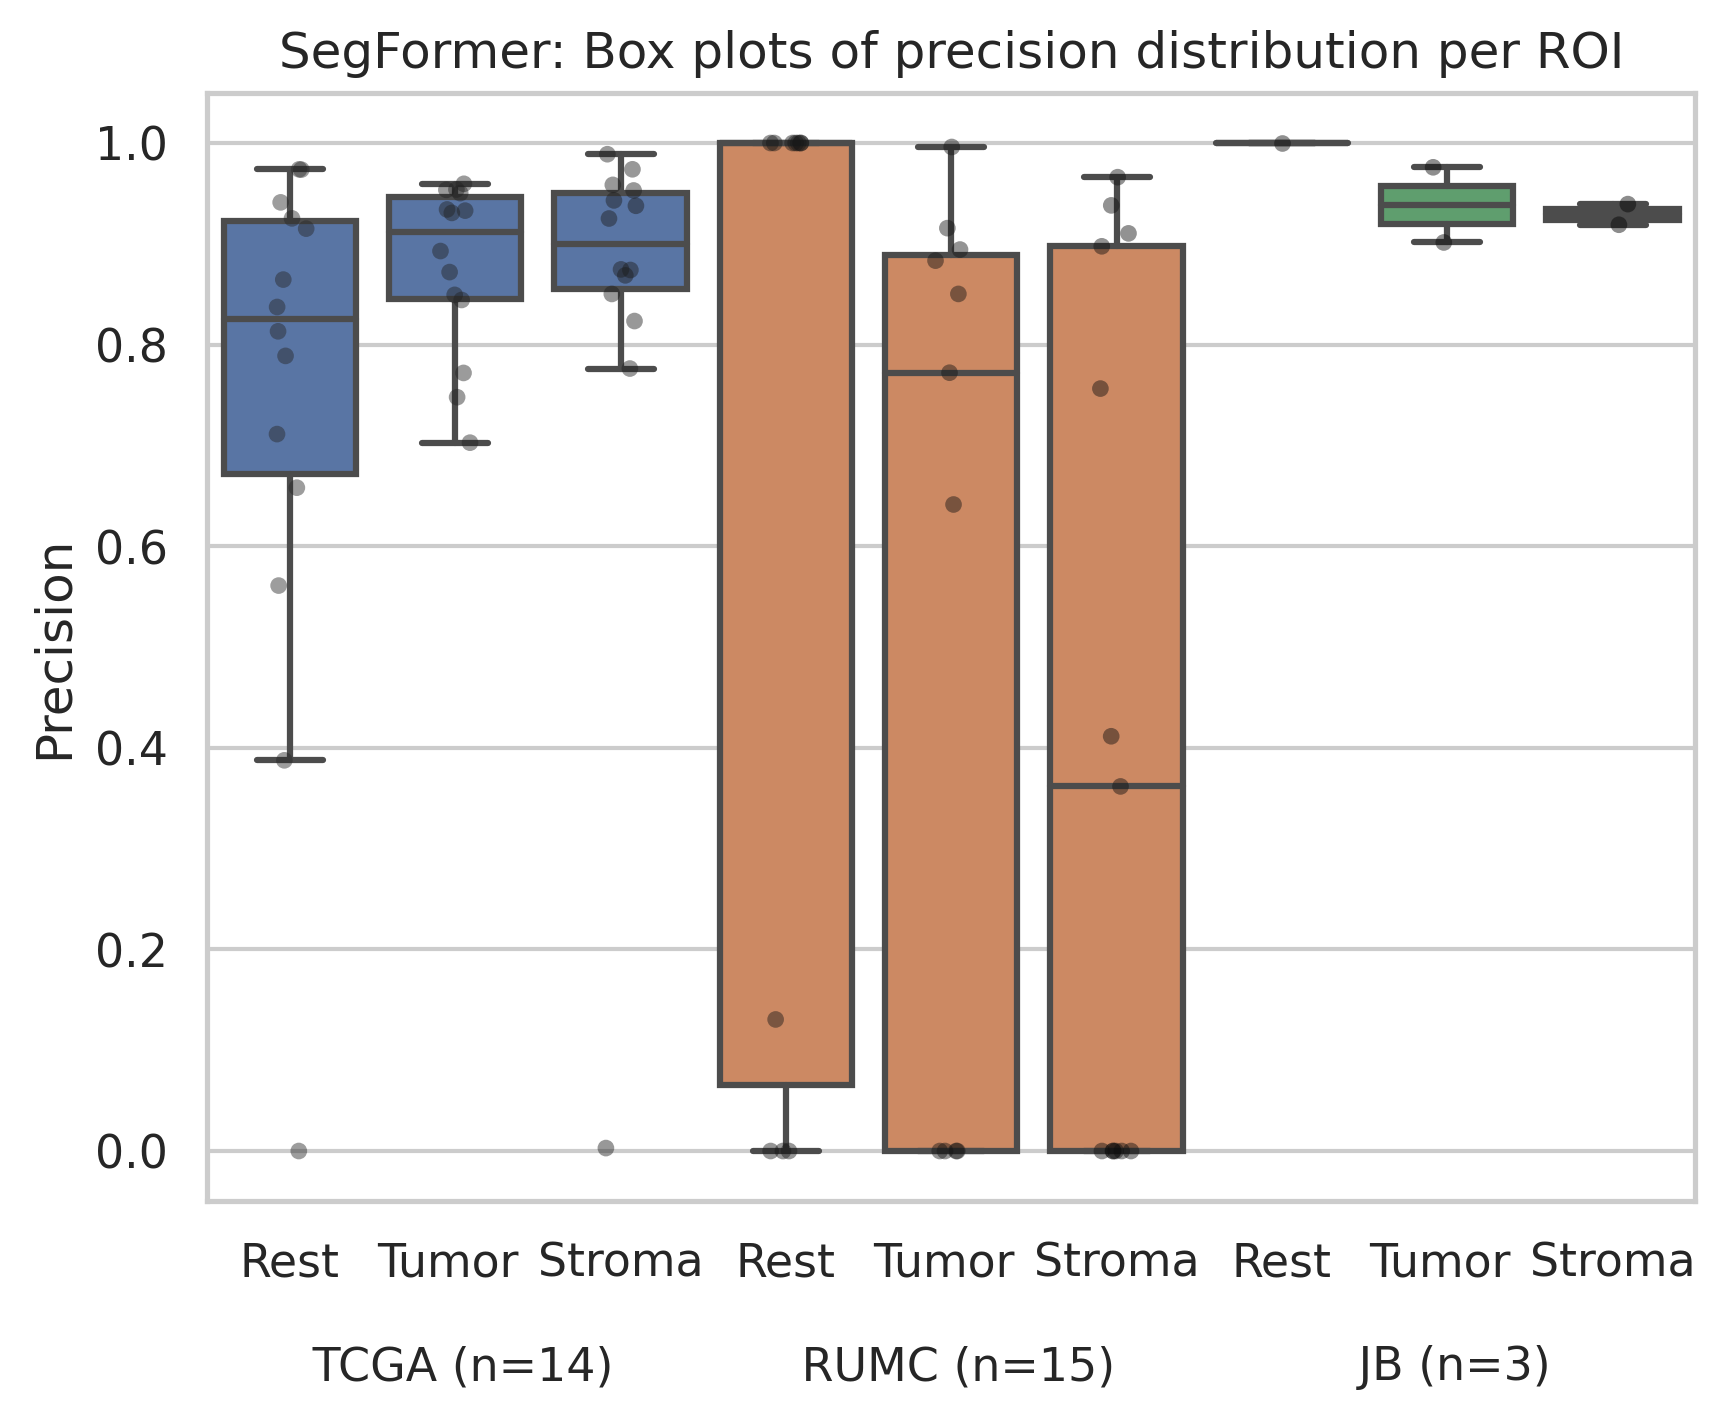
\includegraphics[width=.5\linewidth]{figures/tissue/segformer_prec_roi_wsirois.png}
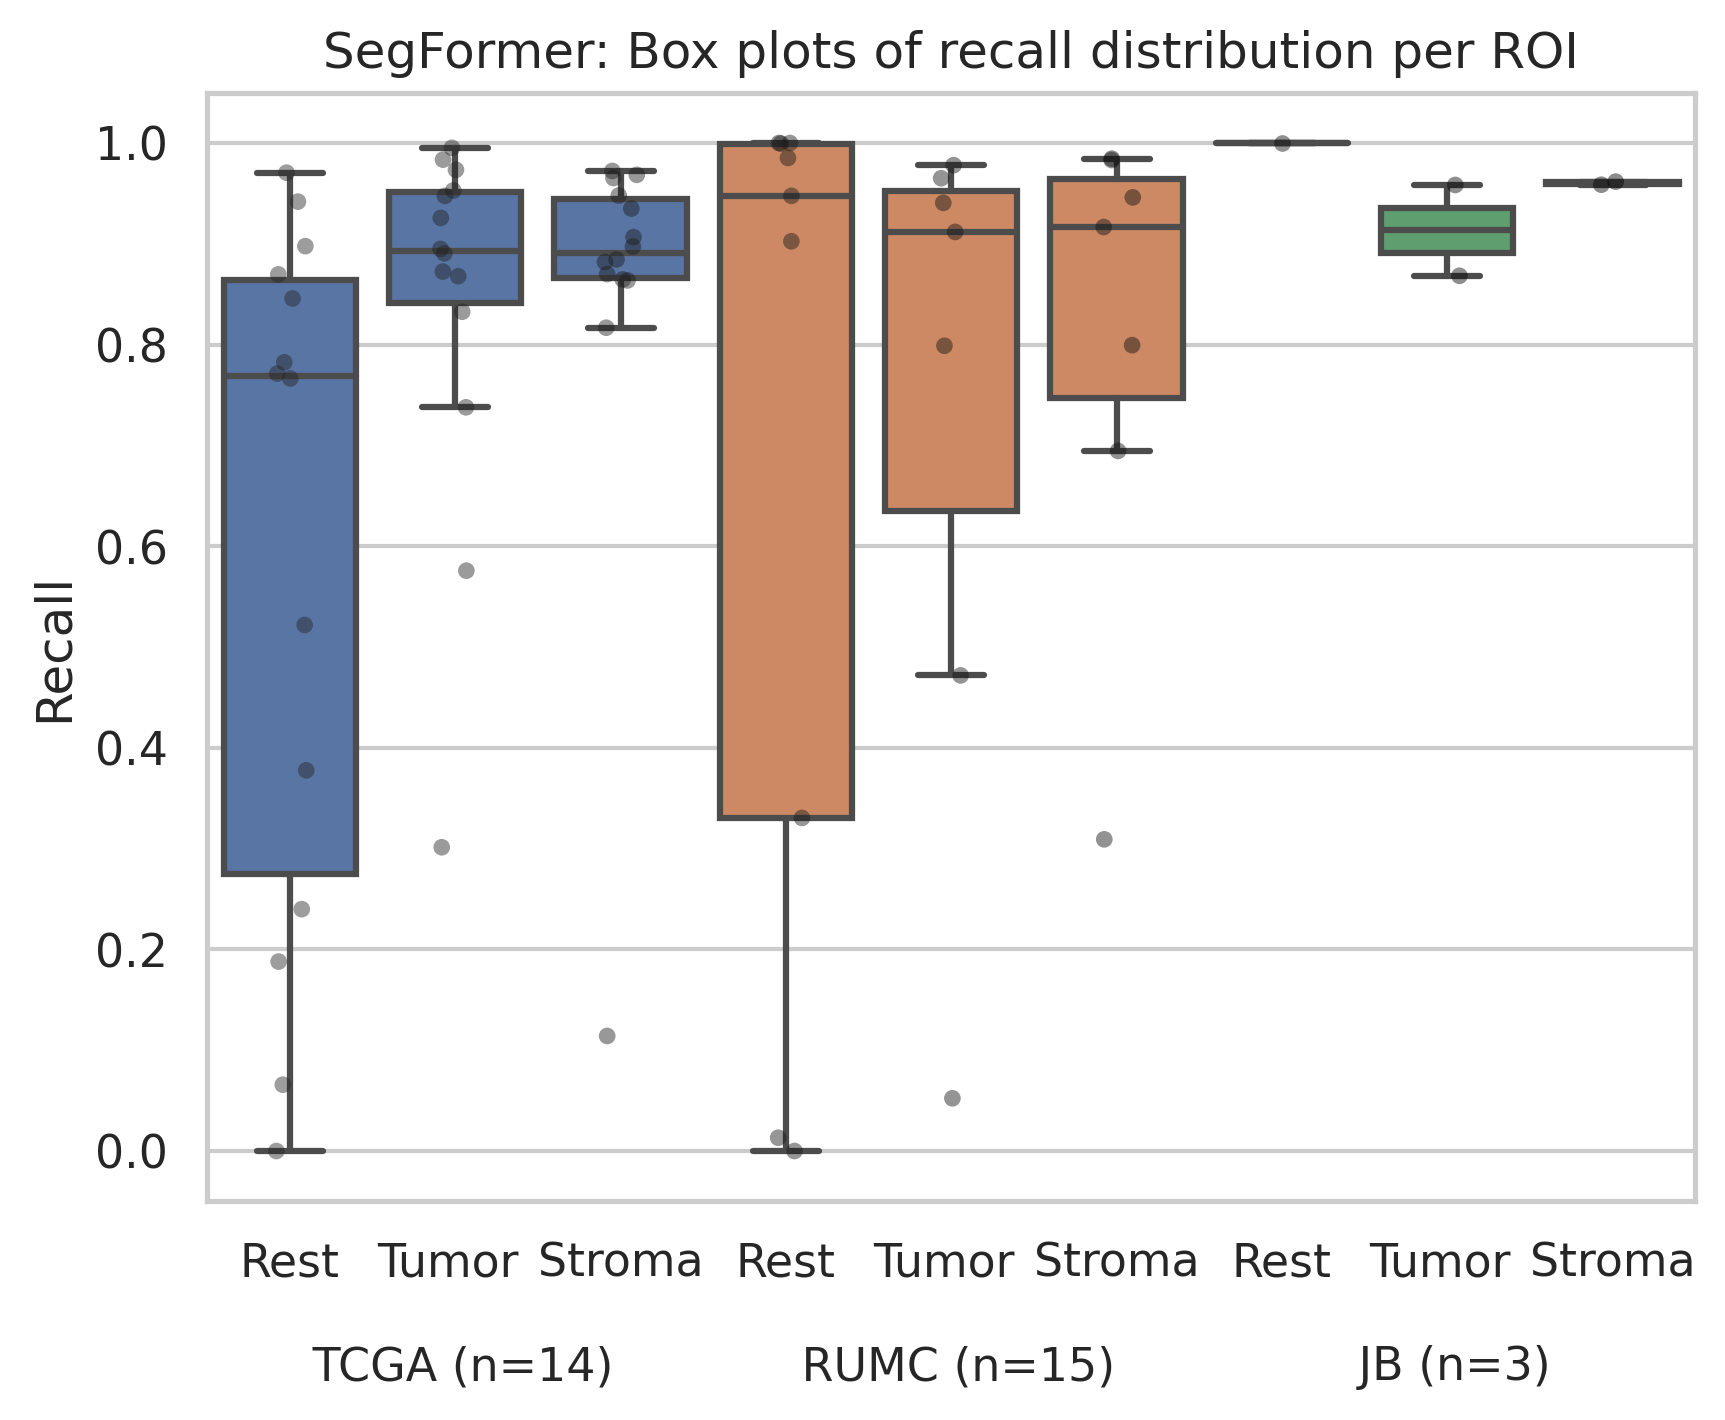
\includegraphics[width=.5\linewidth]{figures/tissue/segformer_recall_roi_wsirois.png}

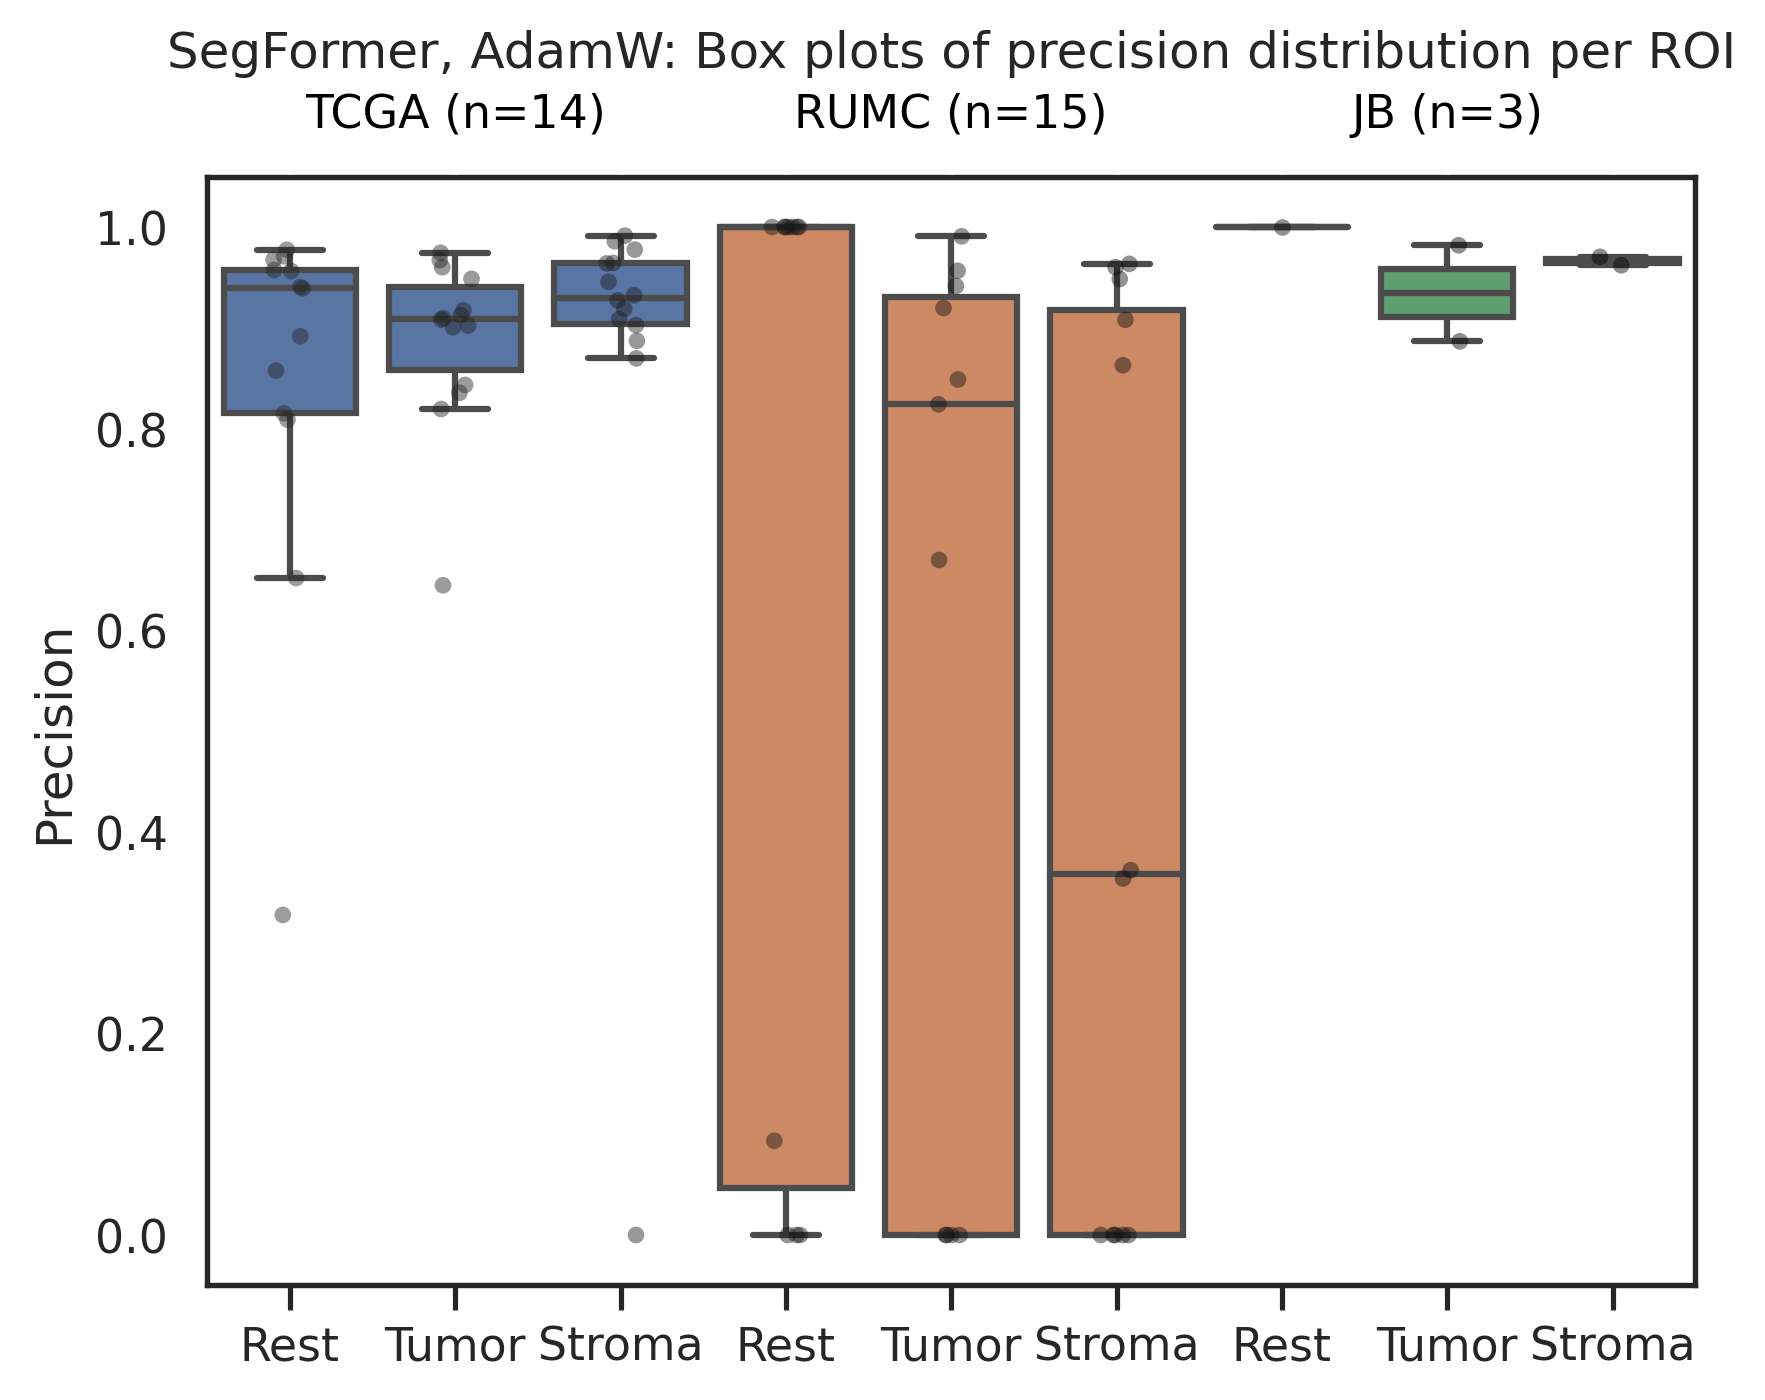
\includegraphics[width=.5\linewidth]{figures/tissue/segformer,_adamw_prec_roi_wsirois.png}
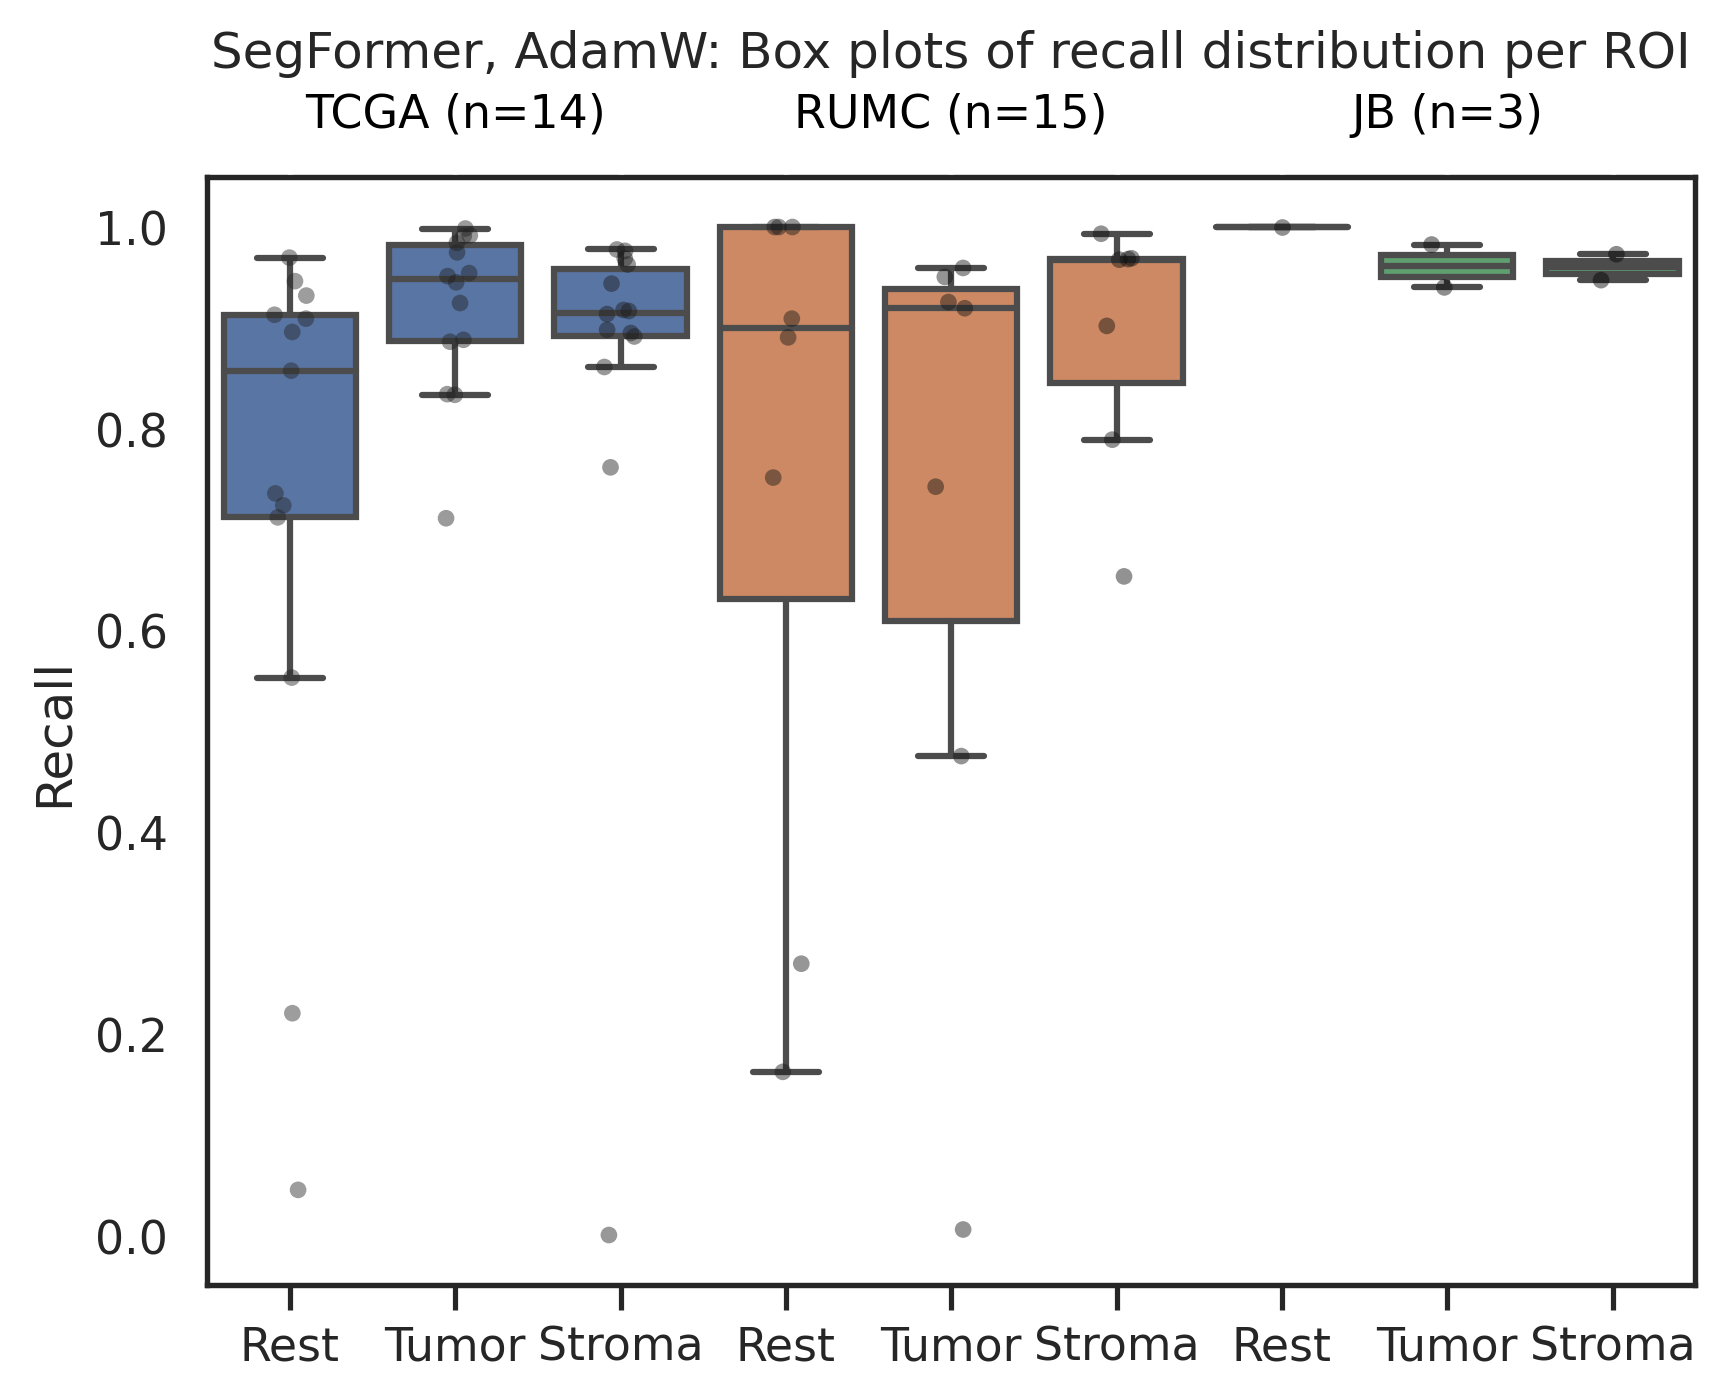
\includegraphics[width=.5\linewidth]{figures/tissue/segformer,_adamw_recall_roi_wsirois.png}
\caption{Boxplots of pixel wise calculated precision and recall across three datastes (TCGA-BRCA, RUMC, JB) and three segmentation labels.}
\label{fig:tissue_pr_r_boxplots}
\end{figure}

\begin{figure}[H]
    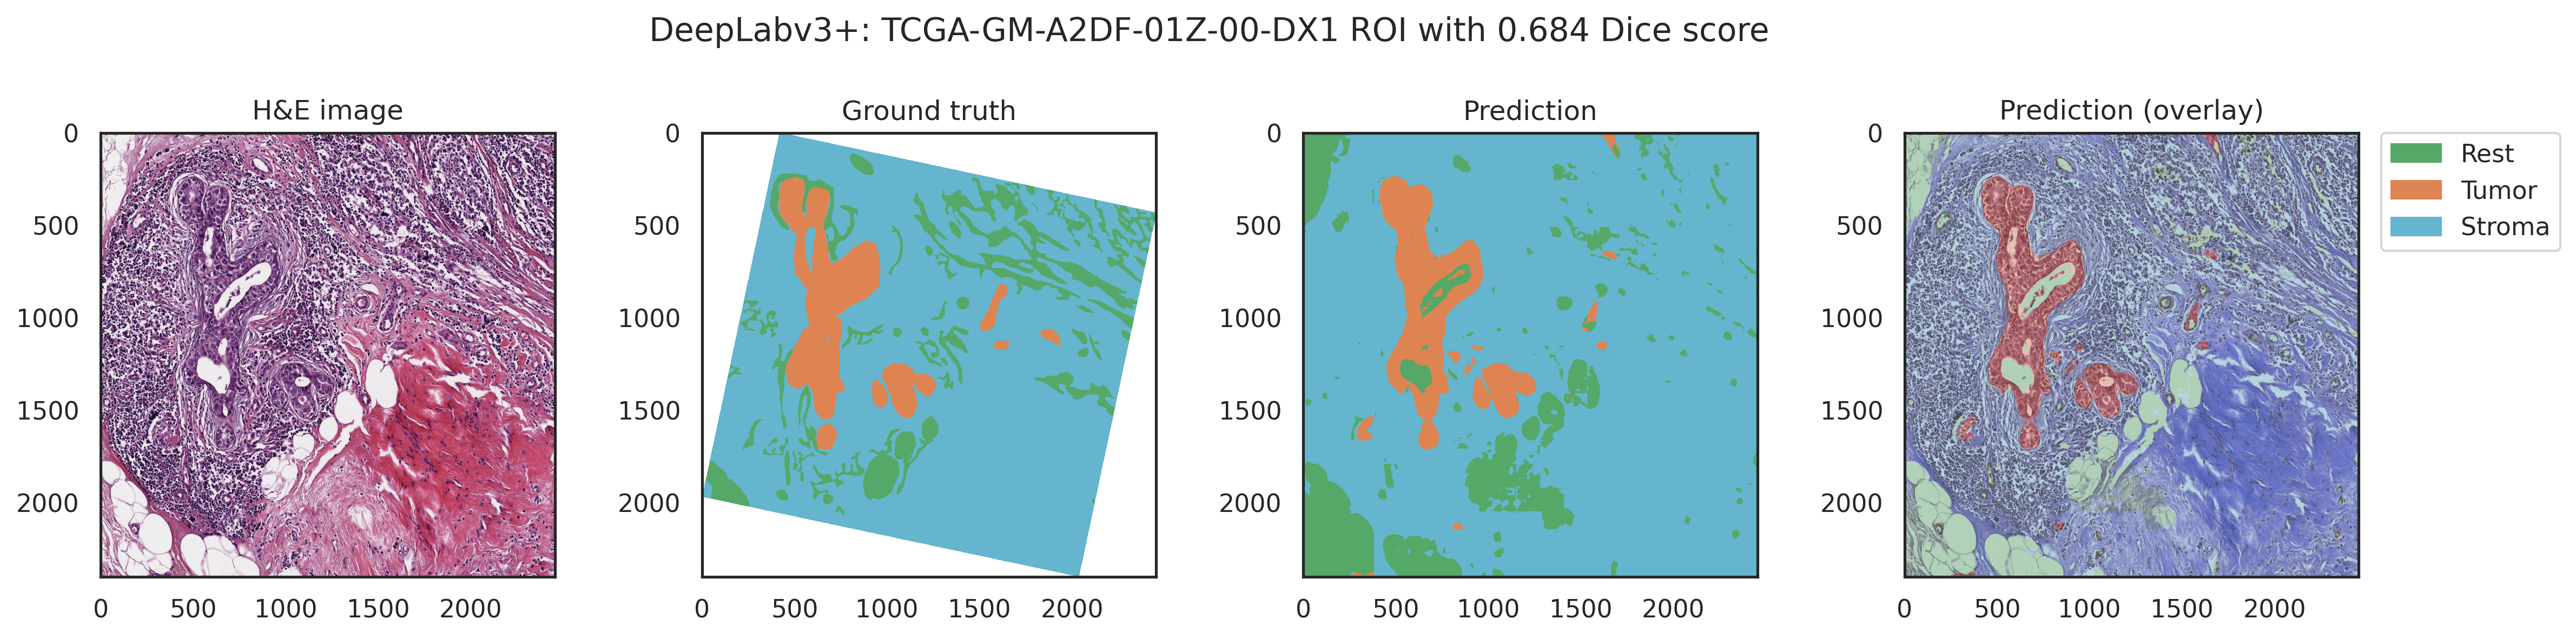
\includegraphics[width=\linewidth]{figures/tissue/deeplabv3+_dice_tcga_TCGA-GM-A2DF-01Z-00-DX1CD0BE6D7-2DB3-4193-84CC-F9BE7BF18CC2_[25322,_21890,_27778,_24293]_check.png}
    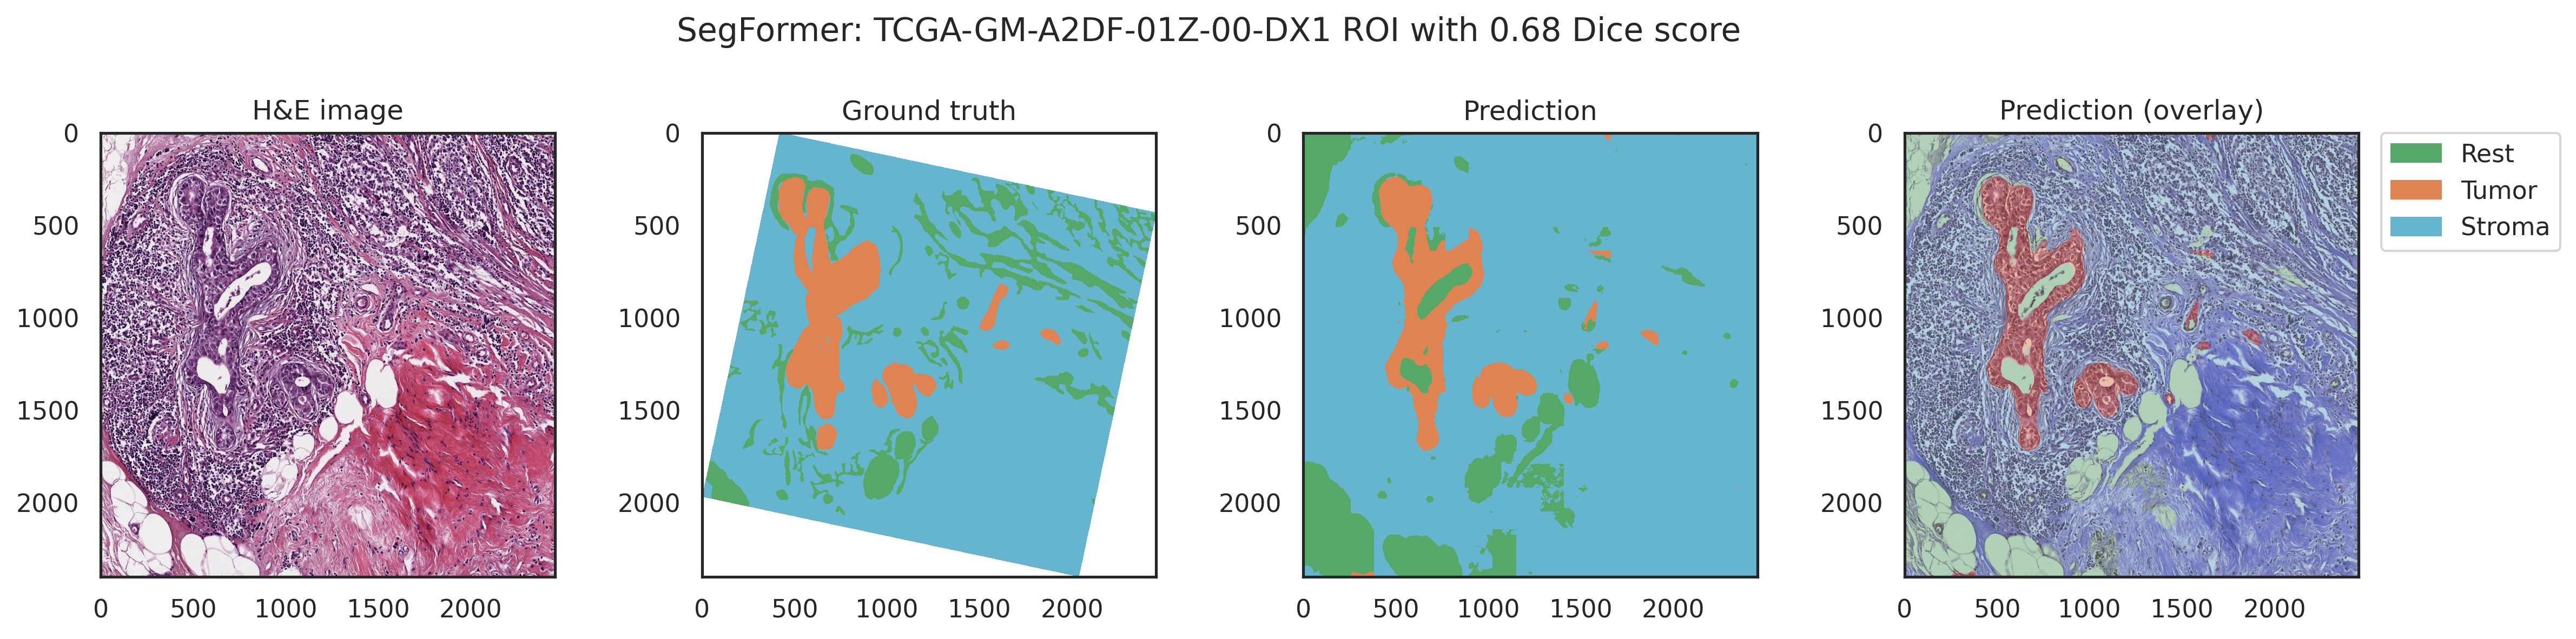
\includegraphics[width=\linewidth]{figures/tissue/segformer_dice_tcga_TCGA-GM-A2DF-01Z-00-DX1CD0BE6D7-2DB3-4193-84CC-F9BE7BF18CC2_[25322,_21890,_27778,_24293]_check.png}
    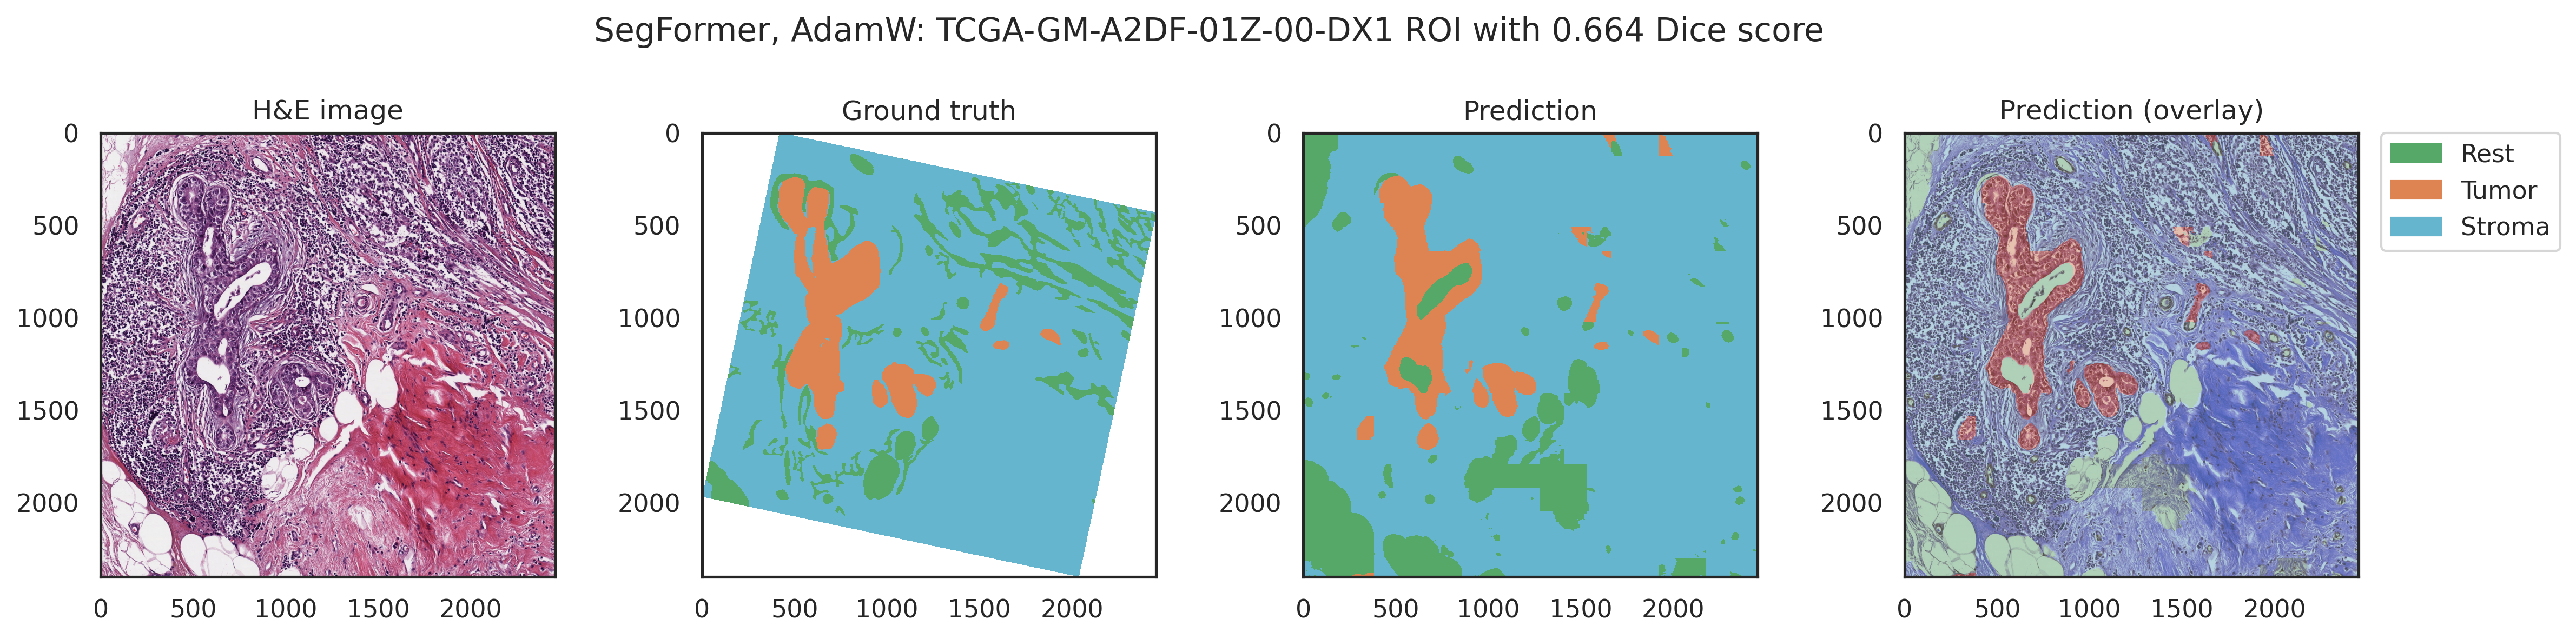
\includegraphics[width=\linewidth]{figures/tissue/segformer,_adamw_dice_tcga_TCGA-GM-A2DF-01Z-00-DX1CD0BE6D7-2DB3-4193-84CC-F9BE7BF18CC2_[25322,_21890,_27778,_24293]_check.png}
    
    \caption{Example of a slightly devalued dice score due to some annotation inaccuracies.}
    \label{fig:TCGA-GM-A2DF}
\end{figure}
    

\begin{figure}[H]
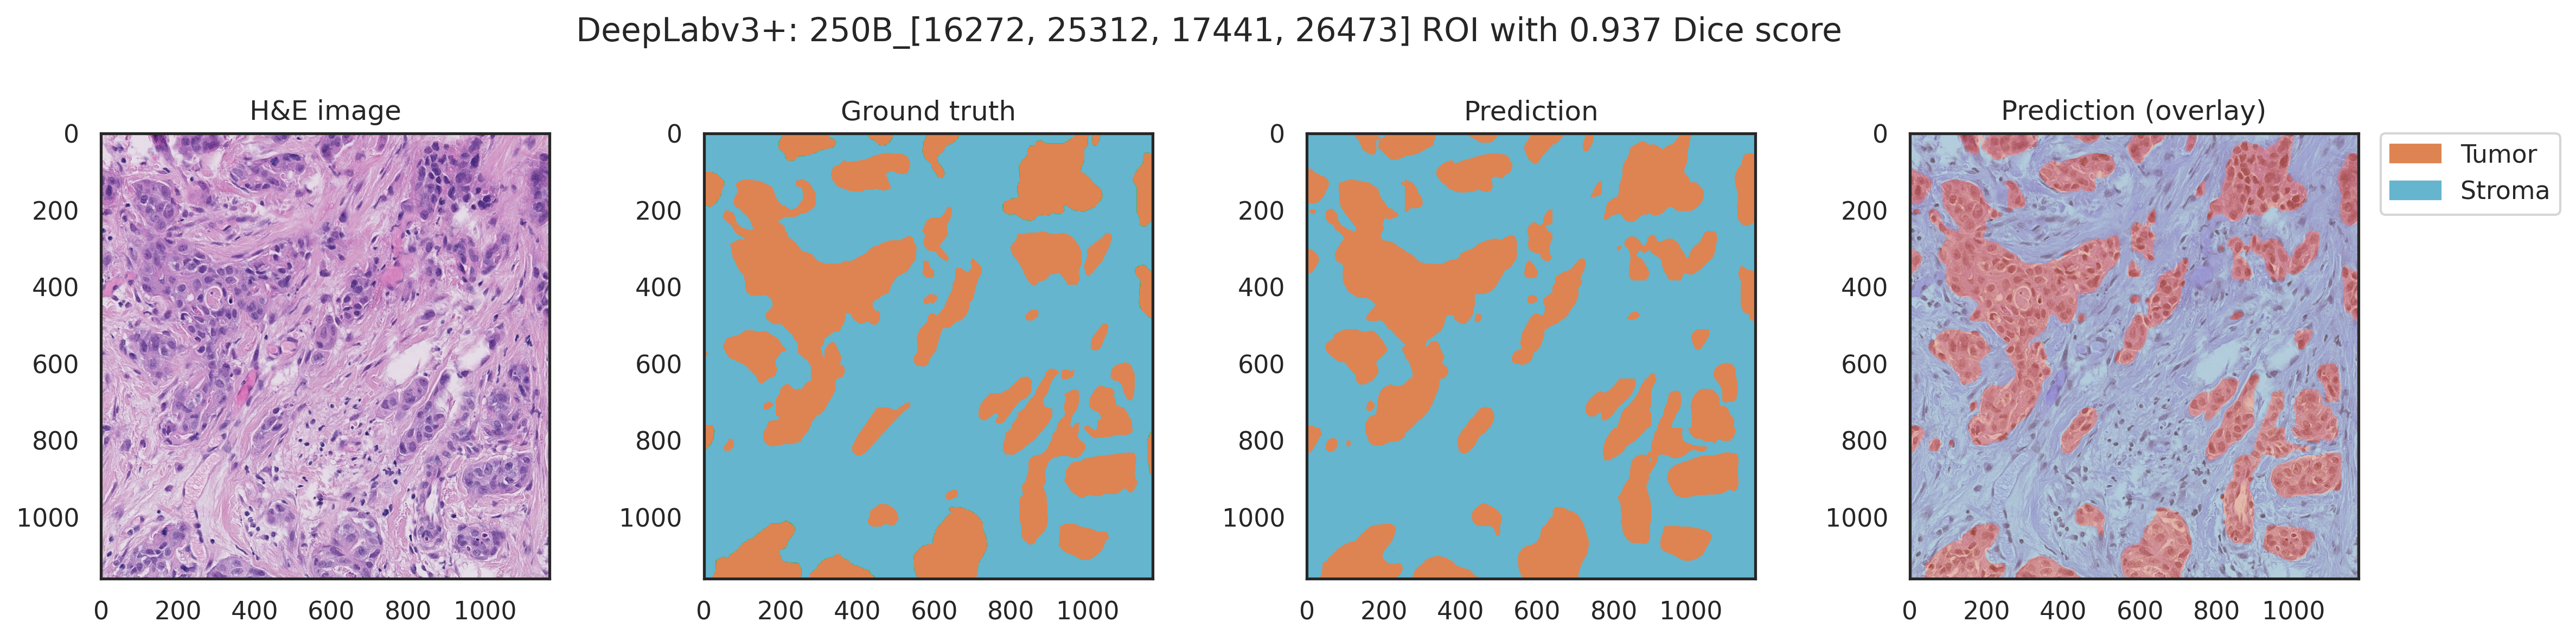
\includegraphics[width=\linewidth]{figures/tissue/deeplabv3+_dice_s_250B_[16272,_25312,_17441,_26473]_check.png}
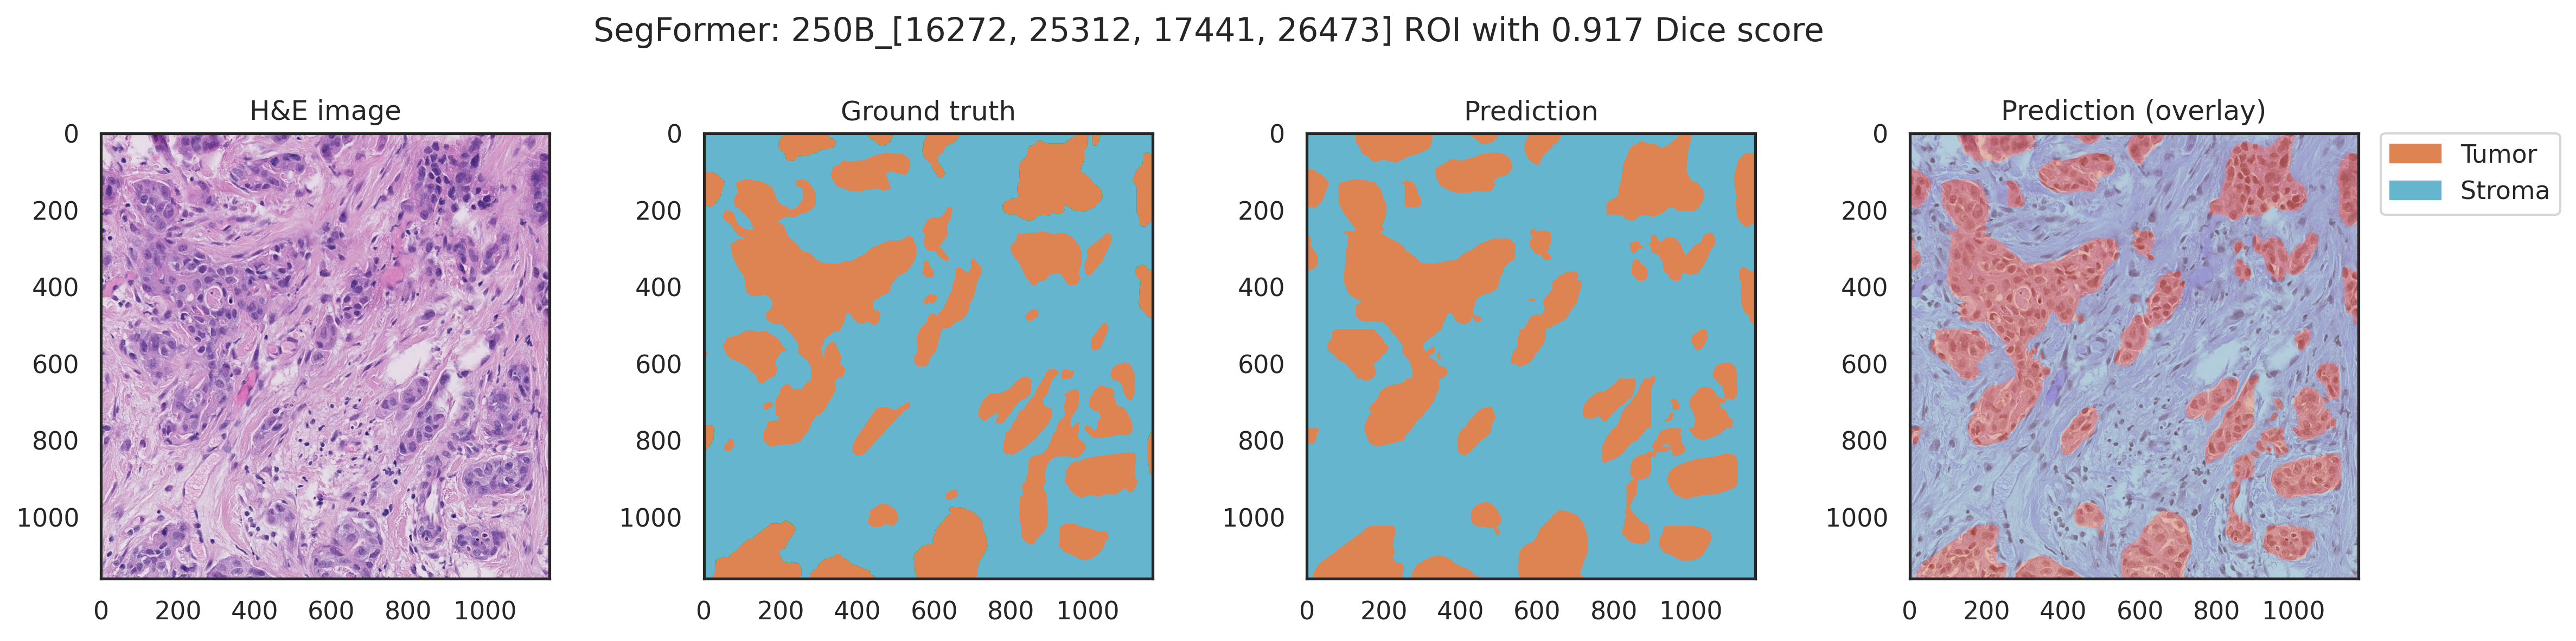
\includegraphics[width=\linewidth]{figures/tissue/segformer_dice_s_250B_[16272,_25312,_17441,_26473]_check.png}
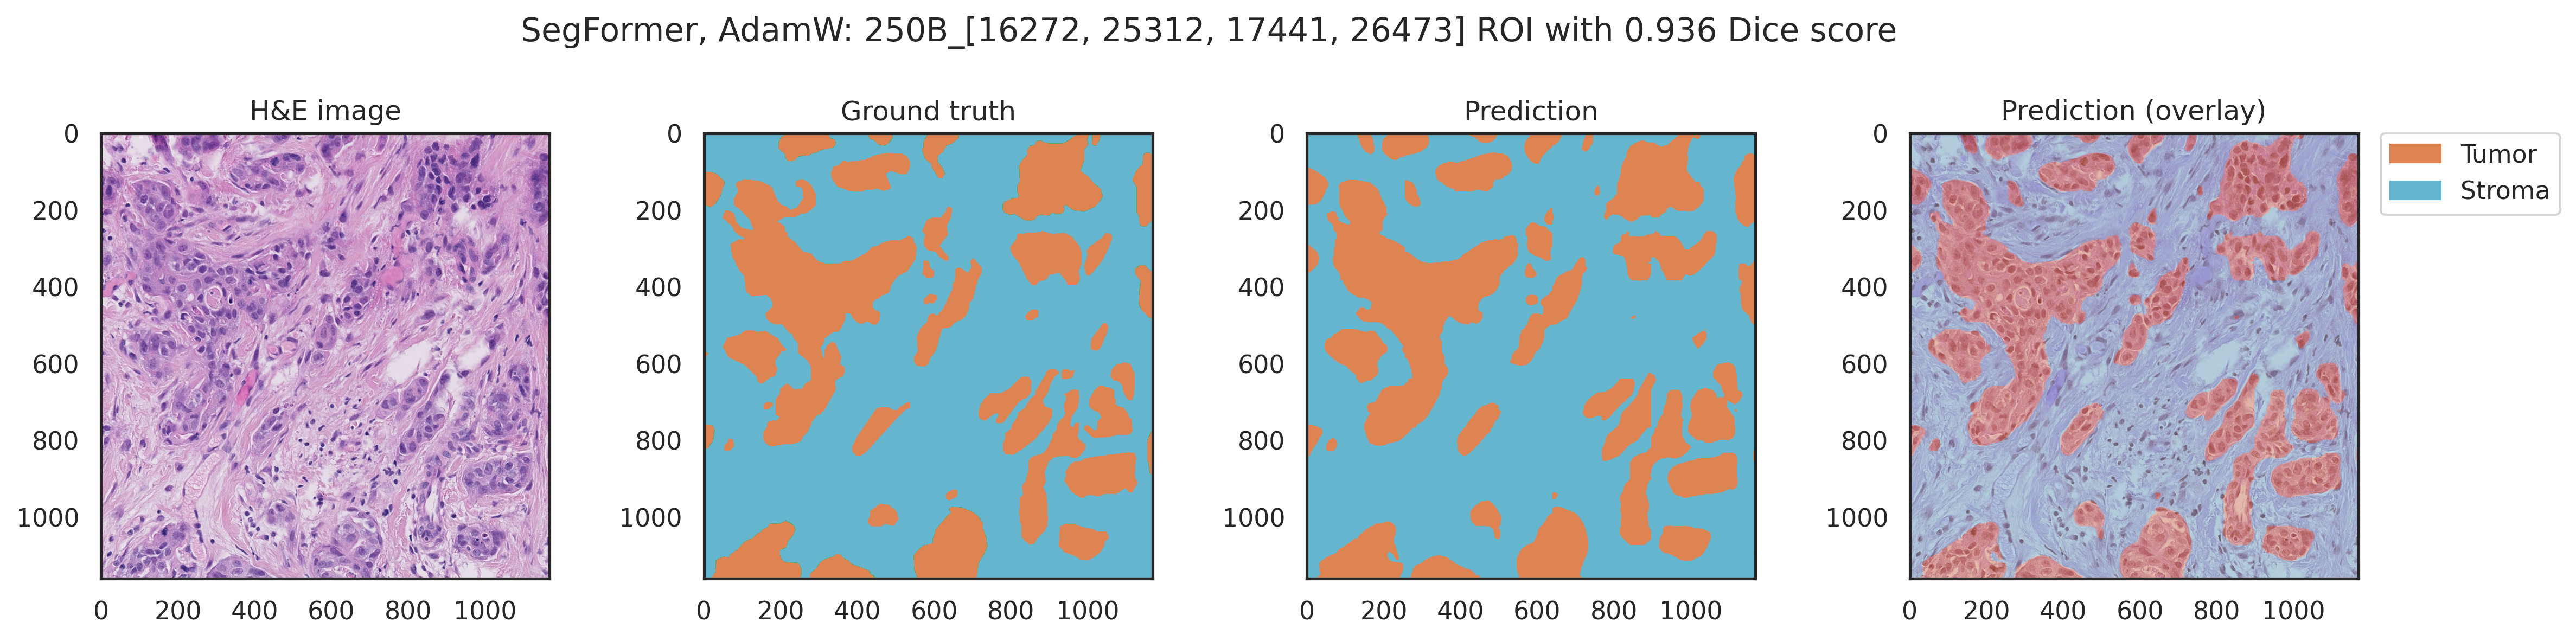
\includegraphics[width=\linewidth]{figures/tissue/segformer,_adamw_dice_s_250B_[16272,_25312,_17441,_26473]_check.png}

\caption{JB S\_250B ROI segmentation result.}
\label{fig:s_250B_1}
\end{figure}

\begin{figure}[H]
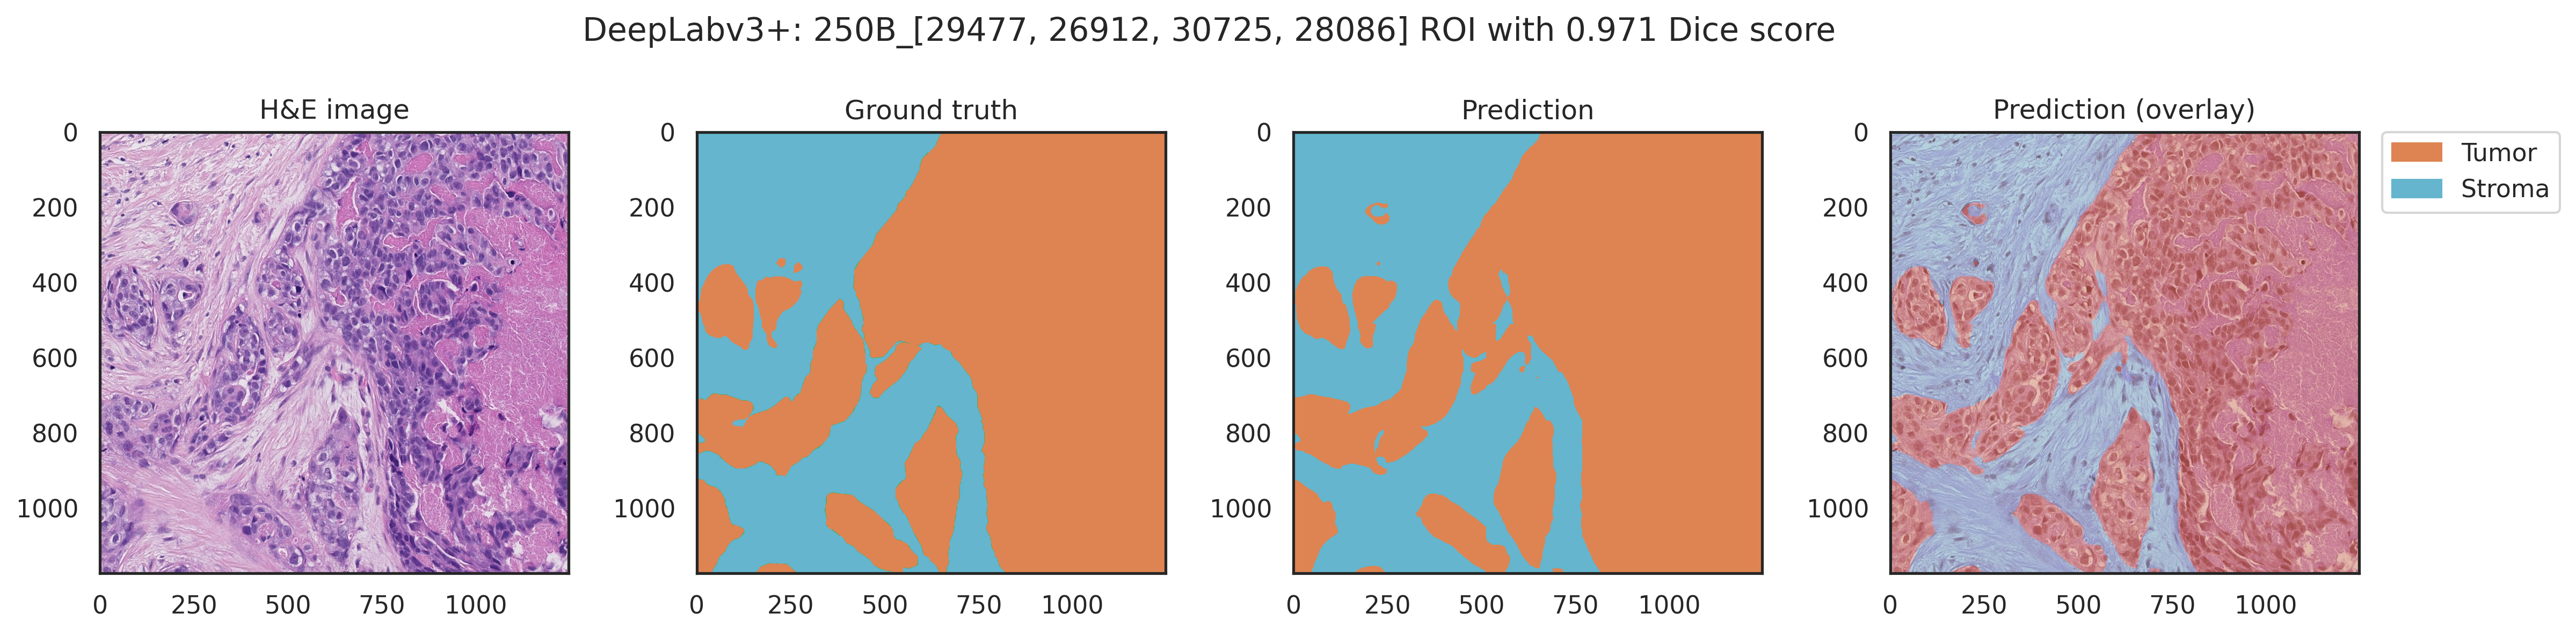
\includegraphics[width=\linewidth]{figures/tissue/deeplabv3+_dice_s_250B_[29477,_26912,_30725,_28086]_check.png}
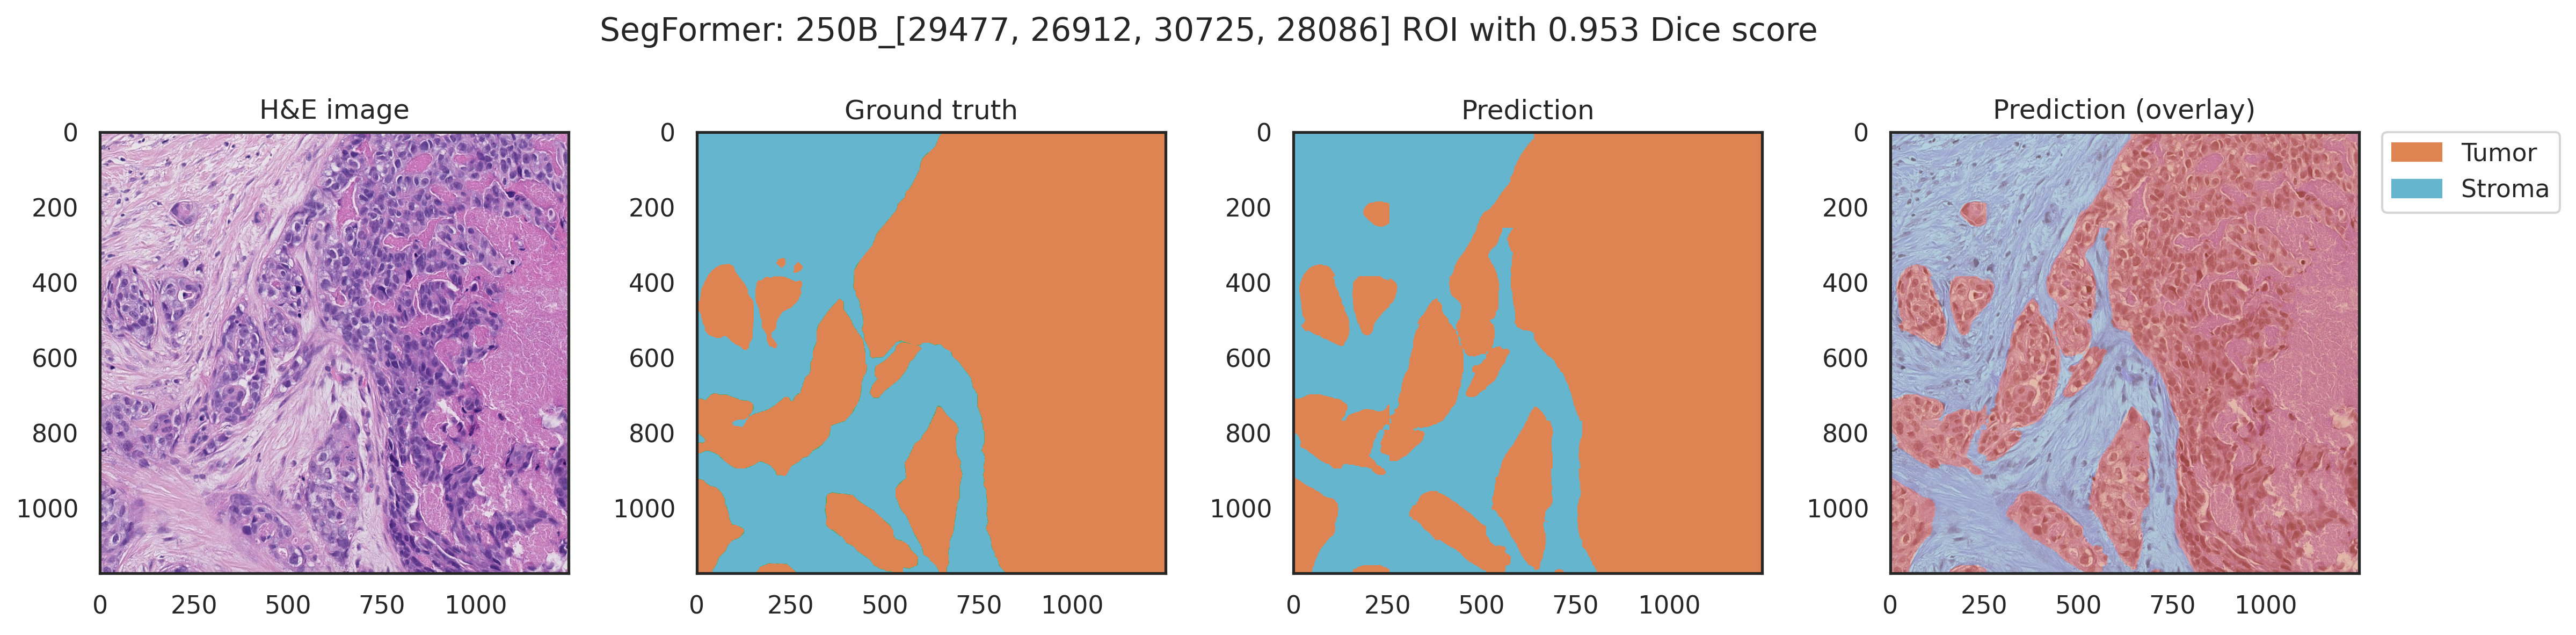
\includegraphics[width=\linewidth]{figures/tissue/segformer_dice_s_250B_[29477,_26912,_30725,_28086]_check.png}
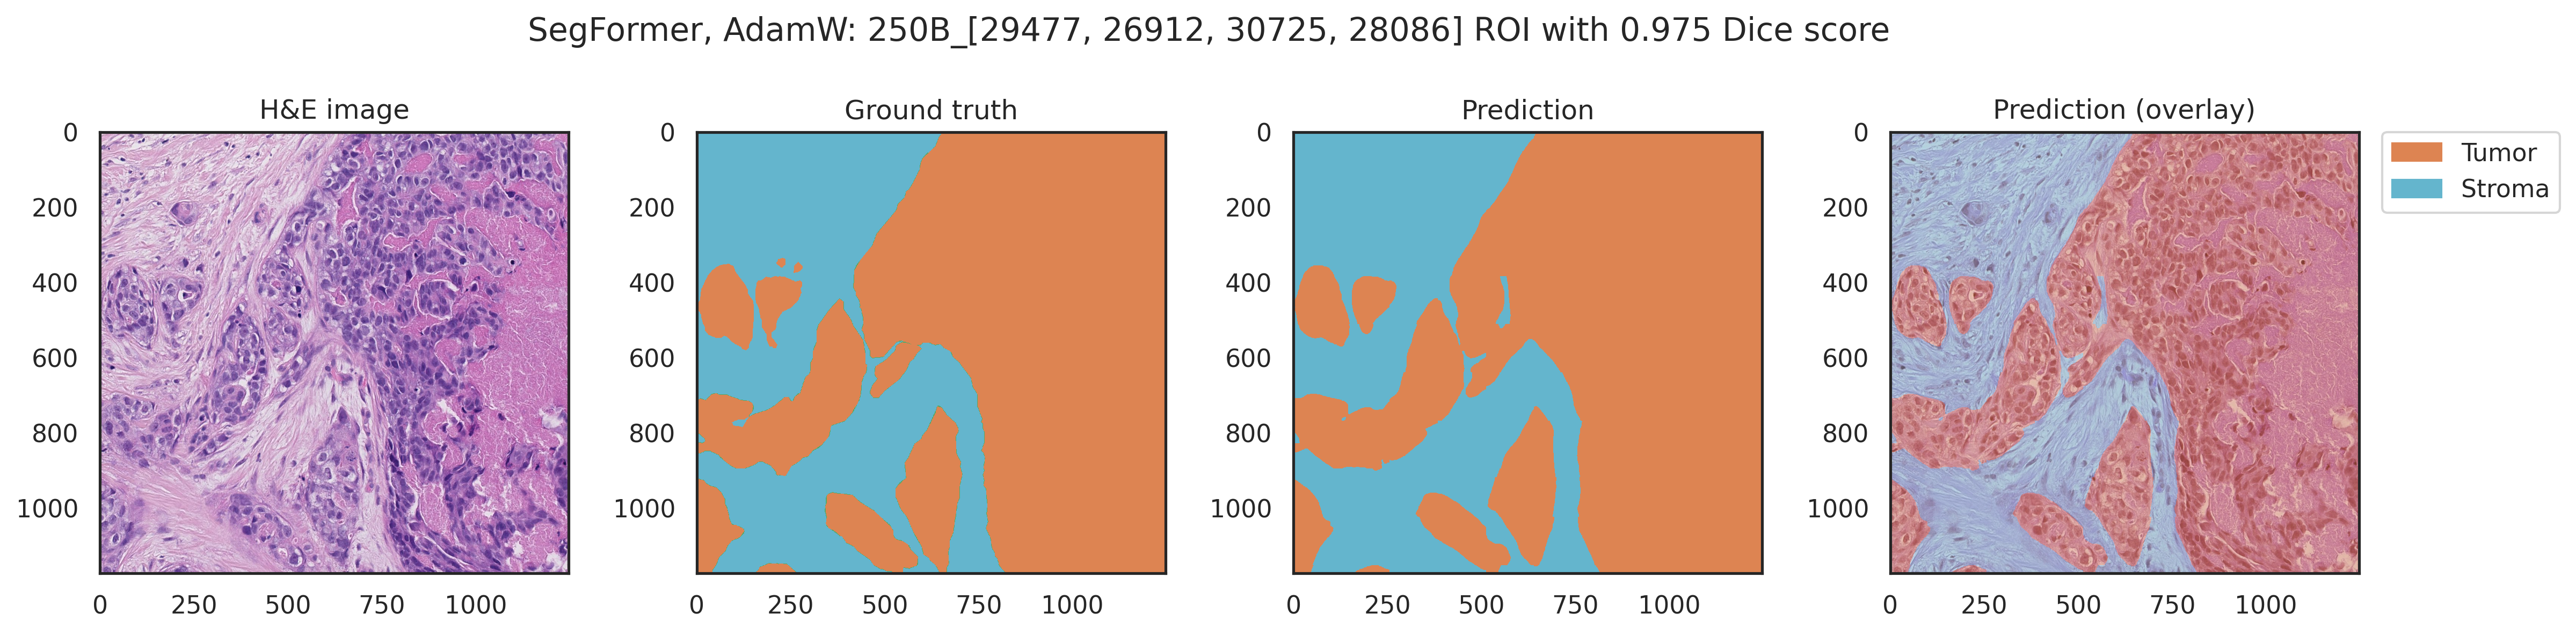
\includegraphics[width=\linewidth]{figures/tissue/segformer,_adamw_dice_s_250B_[29477,_26912,_30725,_28086]_check.png}

\caption{JB S\_250B ROI segmentation result.}
\label{fig:s_250B_2}
\end{figure}

\begin{figure}[H]
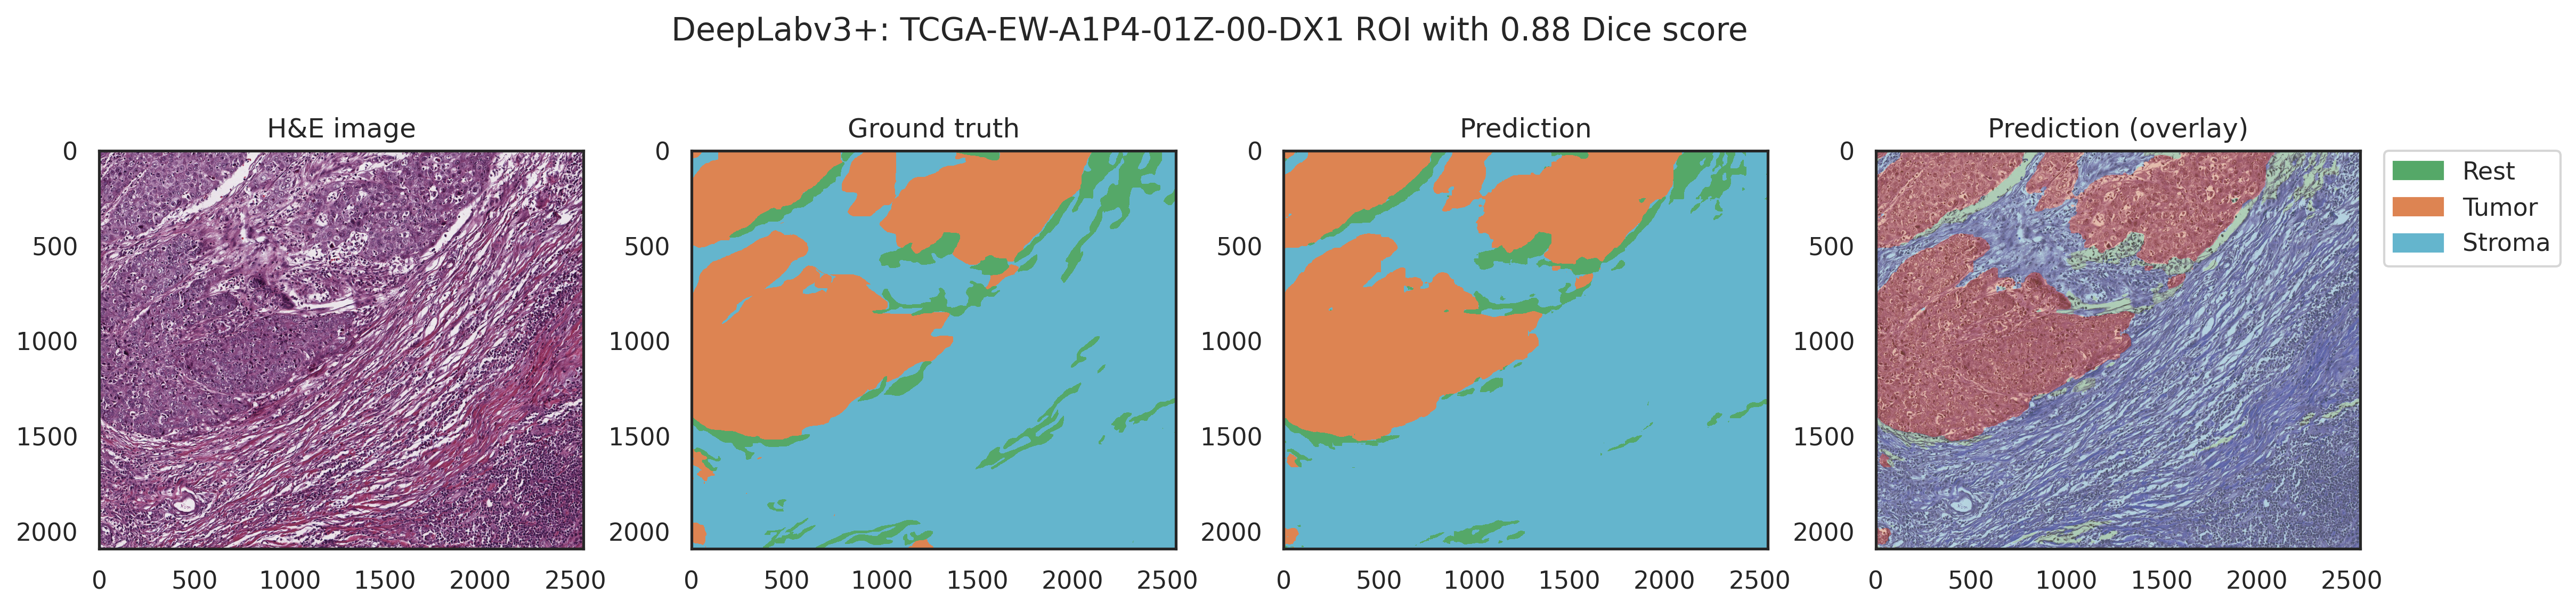
\includegraphics[width=\linewidth]{figures/tissue/deeplabv3+_dice_tcga_TCGA-EW-A1P4-01Z-00-DX13E9AE553-83D4-4B09-AB7F-D096BCE3BC4D_[8630,_17717,_11173,_19809]_check.png}
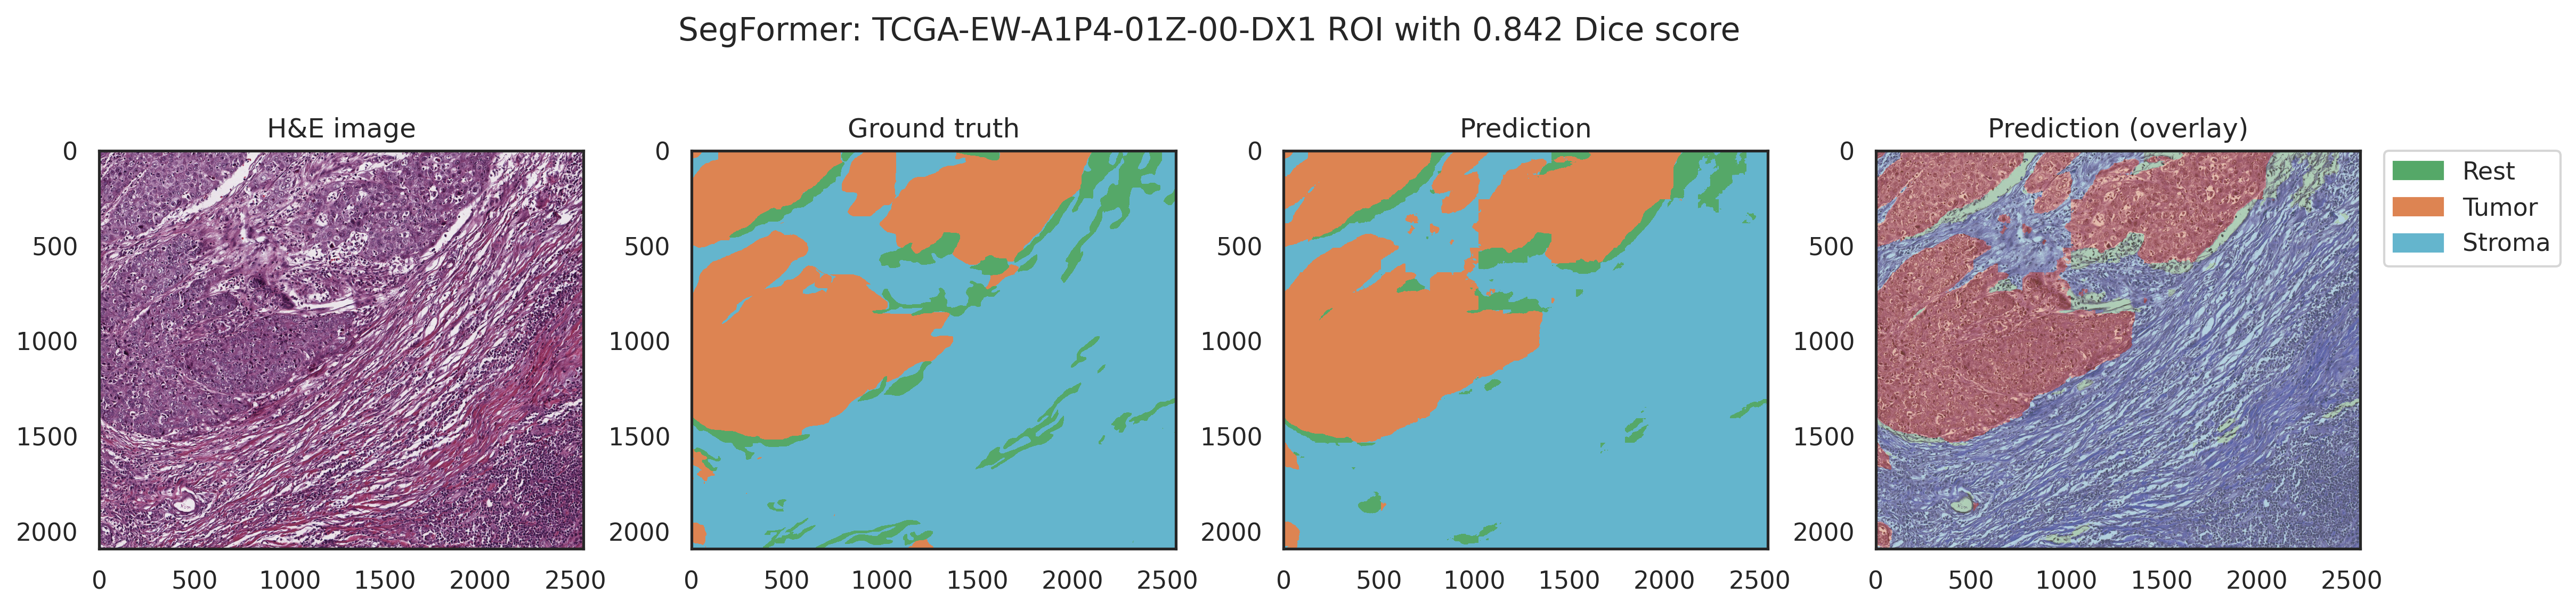
\includegraphics[width=\linewidth]{figures/tissue/segformer_dice_tcga_TCGA-EW-A1P4-01Z-00-DX13E9AE553-83D4-4B09-AB7F-D096BCE3BC4D_[8630,_17717,_11173,_19809]_check.png}
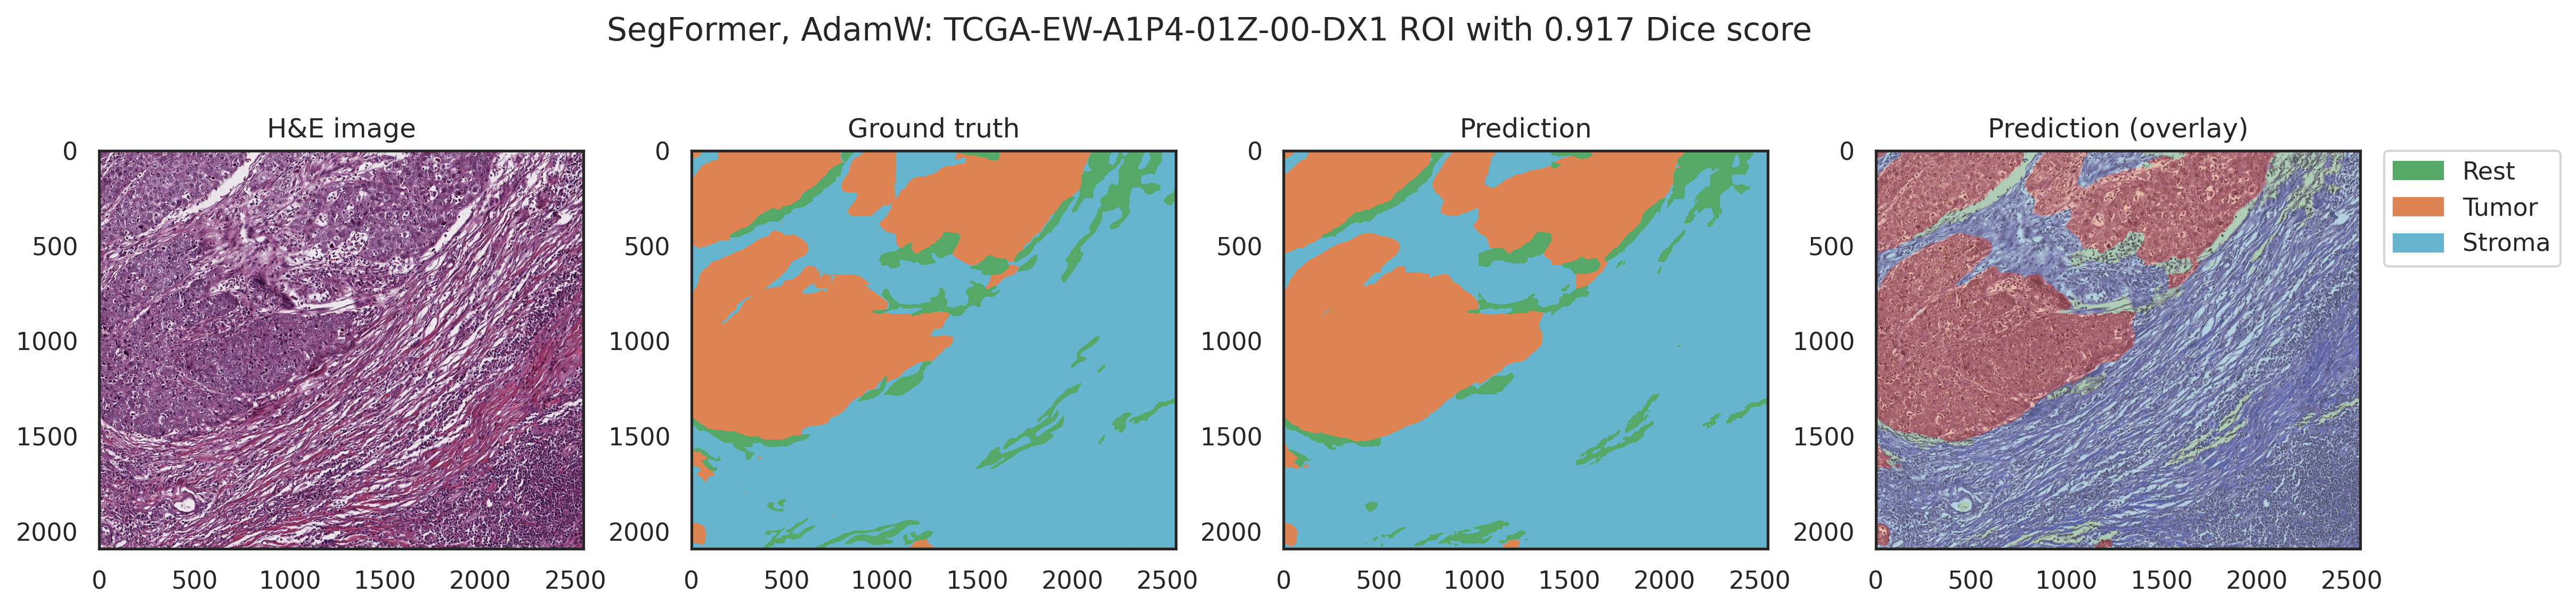
\includegraphics[width=\linewidth]{figures/tissue/segformer,_adamw_dice_tcga_TCGA-EW-A1P4-01Z-00-DX13E9AE553-83D4-4B09-AB7F-D096BCE3BC4D_[8630,_17717,_11173,_19809]_check.png}

\caption{TCGA-EW-A1P4-01Z-00-DX1 ROI segmentation result.}
\label{fig:TCGA-EW-A1P4}
\end{figure}



\section{TILs Segmentation}
TILs segmentation task aimed to segment the RGB input of H\&E stained image at 20$\times$ magnification
(resolution of 0.5 micron-per-pixel) into two prediction maps: TILs and rest.
The split of the patients was used similarly to the previously described in
Tabel~\ref*{tab:patients_sep}. Even though the same patients are present in
this data set, the annotations originate from a different
study which results in a different ROI and patch statistics shown in
Table~\ref*{tab:patch_sep_tils}. The patches were created using a sliding
window approach with 128$\times$128 sized patches
and stride equals 100. The ROIs that were smaller than 128$\times$128
were padded. The additional rotation augmentation was applied,
by rotating each patch 5 times at 9 degrees each.
The column "Number of patches that include rest" in Table~\ref*{tab:patch_sep_tils}
seems excessive, but was still added
for better data comprehension: the ROIs for TILs segmentation are either
completely annotated as rest or include occasional TILs masks.
%This unequal distribution of the classes cause the dataset to be imbalanced.

\begin{table}[h!]
    \centering
    \begin{tabular}{ l c c c c c c c }
        \hline
        & \multirow{2}{*}{slides} & \multirow{2}{*}{ROIs}& \multirow{2}{*}{patches}& \multicolumn{4}{c}{Number of patches that include}\\ 
        \cline{5-8}
        & & & & TILs & Rest & 1 class & 2 classes \\
        \hline
        Train & 156 & 1\,552 & 106\,974 & 35\,433 & 106\,974 & 71\,541 & 35\,433\\
         &  &  &  & (33\%) & (100\%) & (67\%) & (33\%)  \\
        Validation & 20 & 154 & 15\,518 & 14\,164 & 15\,518 & 5\,638 & 3\,734 \\
         &  &  &  & (27\%) & (100\%) & (60\%) & (40\%)\\
        Test & 19 & 173 & 9\,372 & 3\,734 & 9\,372& 11\,354 & 4\,164\\
         &  &  &  & (40\%) & (100\%) & (73\%) & (27\%)\\
        \hline
        & 195 & 1\,879 & 131\,864 &  &  &  & \\
    \end{tabular}
    \caption{\label{tab:patch_sep_tils} Overview of patches that were split into train, validation,
    and test sets for TILs segmentation. The percentages indicate the fraction of a specific conditioned
    group of patches to the number of all patches in the "patches" column.}
\end{table}

The model architectures and their parameters were used as described in~\ref*{res_tissue_segm}:
DeepLabv3+, SegFormer with Adam optimizer, and SegFormer with AdamW. An important
change is an increased batch size of 128, which was allowed due to smaller patch
sizes of 128$\times$128. In the model overview in Table~\ref*{tab:tils_perform}
the number of parameters and
iterations remain the same. FLOPs values are dependent on input shape, therefore
it was expected to drop since the input is smaller.
It is aslo noticed that for TILs segmentation the runtime between all three models
becomes comparable in contrast to tissue segmentation (Table~\ref*{tab:tissue_perform}).

\begin{table}[h!]
    \centering
    \begin{tabular}{ l c c c c c c c c}
        \hline
        Model & FLOPs & Params & Iterations & Runtime & F1 score & Precision & Recall\\
        \hline
        DeepLabv3+ & 11.04 & 43.58 M & 160 K & 2d 8h 36m & 0.49 & 0.58 & 0.43\\
        SegFormer & 3.24 & 81.97 M & 160 K  & 2d 11h 36m & 0.62 & 0.62 & 0.33\\
        SegFormer, & \multirow{2}{*}{3.24} & \multirow{2}{*}{81.97 M} & \multirow{2}{*}{160 K} & \multirow{2}{*}{2d 15h 19m} & \multirow{2}{*}{\textbf{0.66}} & \multirow{2}{*}{0.64} & \multirow{2}{*}{0.69}\\
        AdamW & & & & & & & & \\
        \hline
    \end{tabular}
\caption{\label{tab:tils_perform} Overview of the trained TILs segmentation models. The runtime is given for a training on one GPU NVIDIA A100 SXM4.}
\end{table}

For proper evaluation the predicted TILs segmentation needed to be reduced to TILs
centers (one pixel) that can be then further matched to ground truth.
To get optimal centers of predicted TILs, non-maximum suppression was applied on
posterior images that were clipped between 0 and 255. The search for the best-fitted
parameter of kappa (threshold) and kernel size was completed on the validation set.
As pictured in Figure~\ref*{fig:kappas} there were multiple experiments performed
with kernel sizes  in [1, 3, 5, 7, 9, 11, 13] and multiple kappas. The highest value of
kappa was the median value over all posteriors. The consecutive values were the
two power fractions of the median. Figure~\ref*{fig:kappas} includes two images
for DeepLabv3+ (first in the first row and first in the second row) to provide a
zoomed look of the tighter range. As a result, the best parameters on the validation
set were chosen as kappa=21, kernel size=9 for DeepLabv3+ and kappa=64, kernel size=5
for SegFormer-based methods. The resulting centers were matched to
the ground truth by applying the Hungarian algorithm that found the best assignment
to match ground truth TILs with predicted ones. The allowed maximum distance for a
match of predicted with ground truth TILs was set to 5 \textmu m.

\begin{figure}[h!]
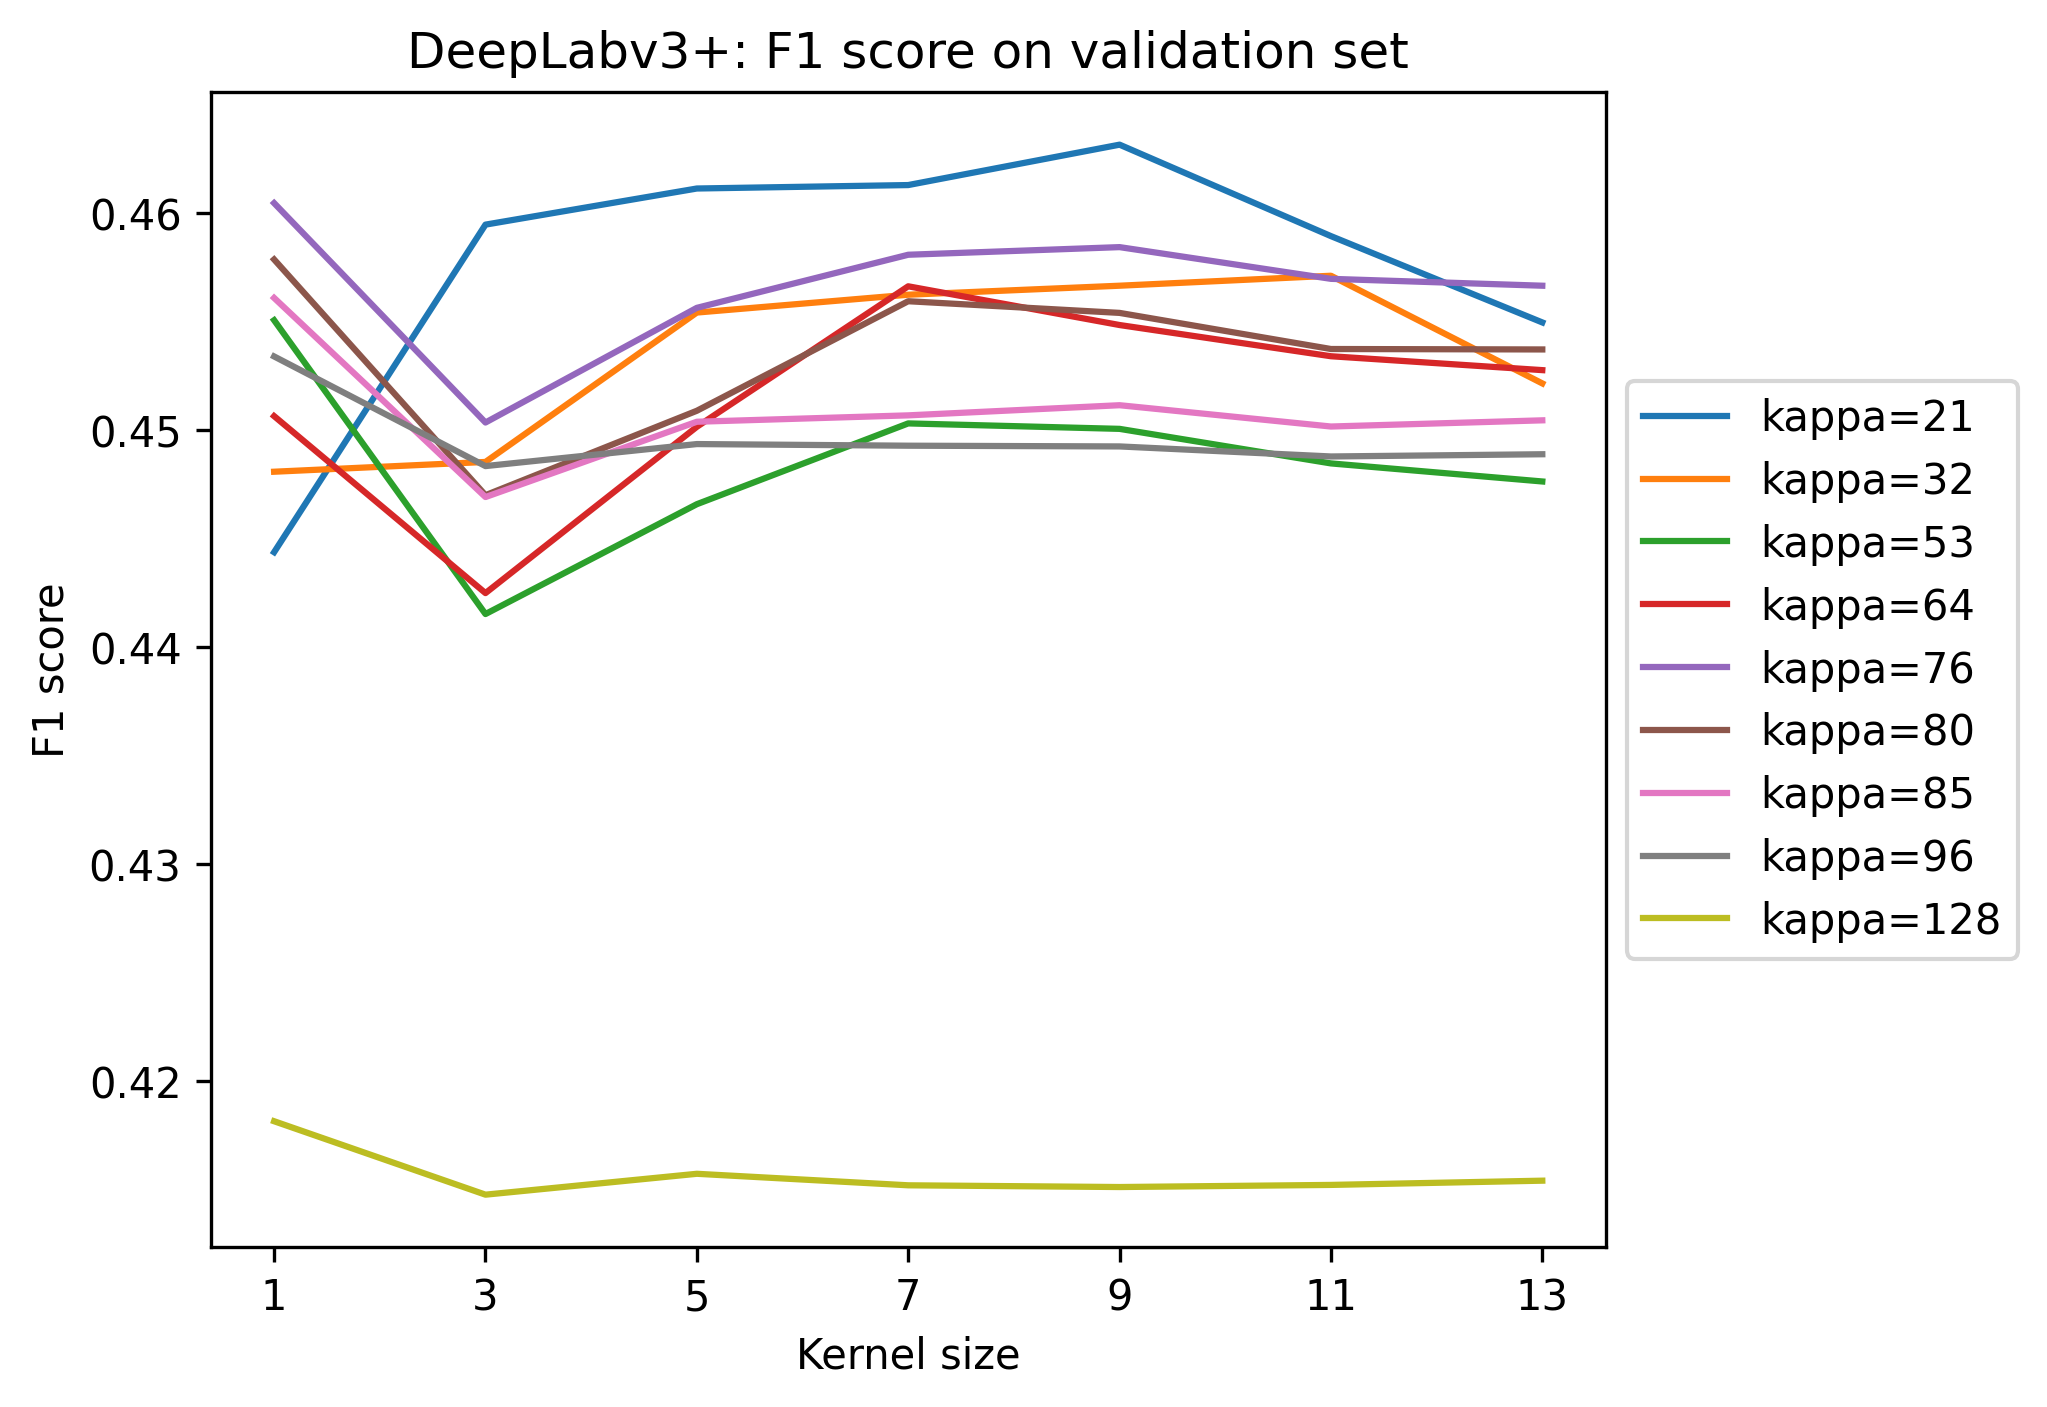
\includegraphics[width=.5\linewidth]{figures/tils/deeplabv3+_f1_kappas_kernels_plot.png}
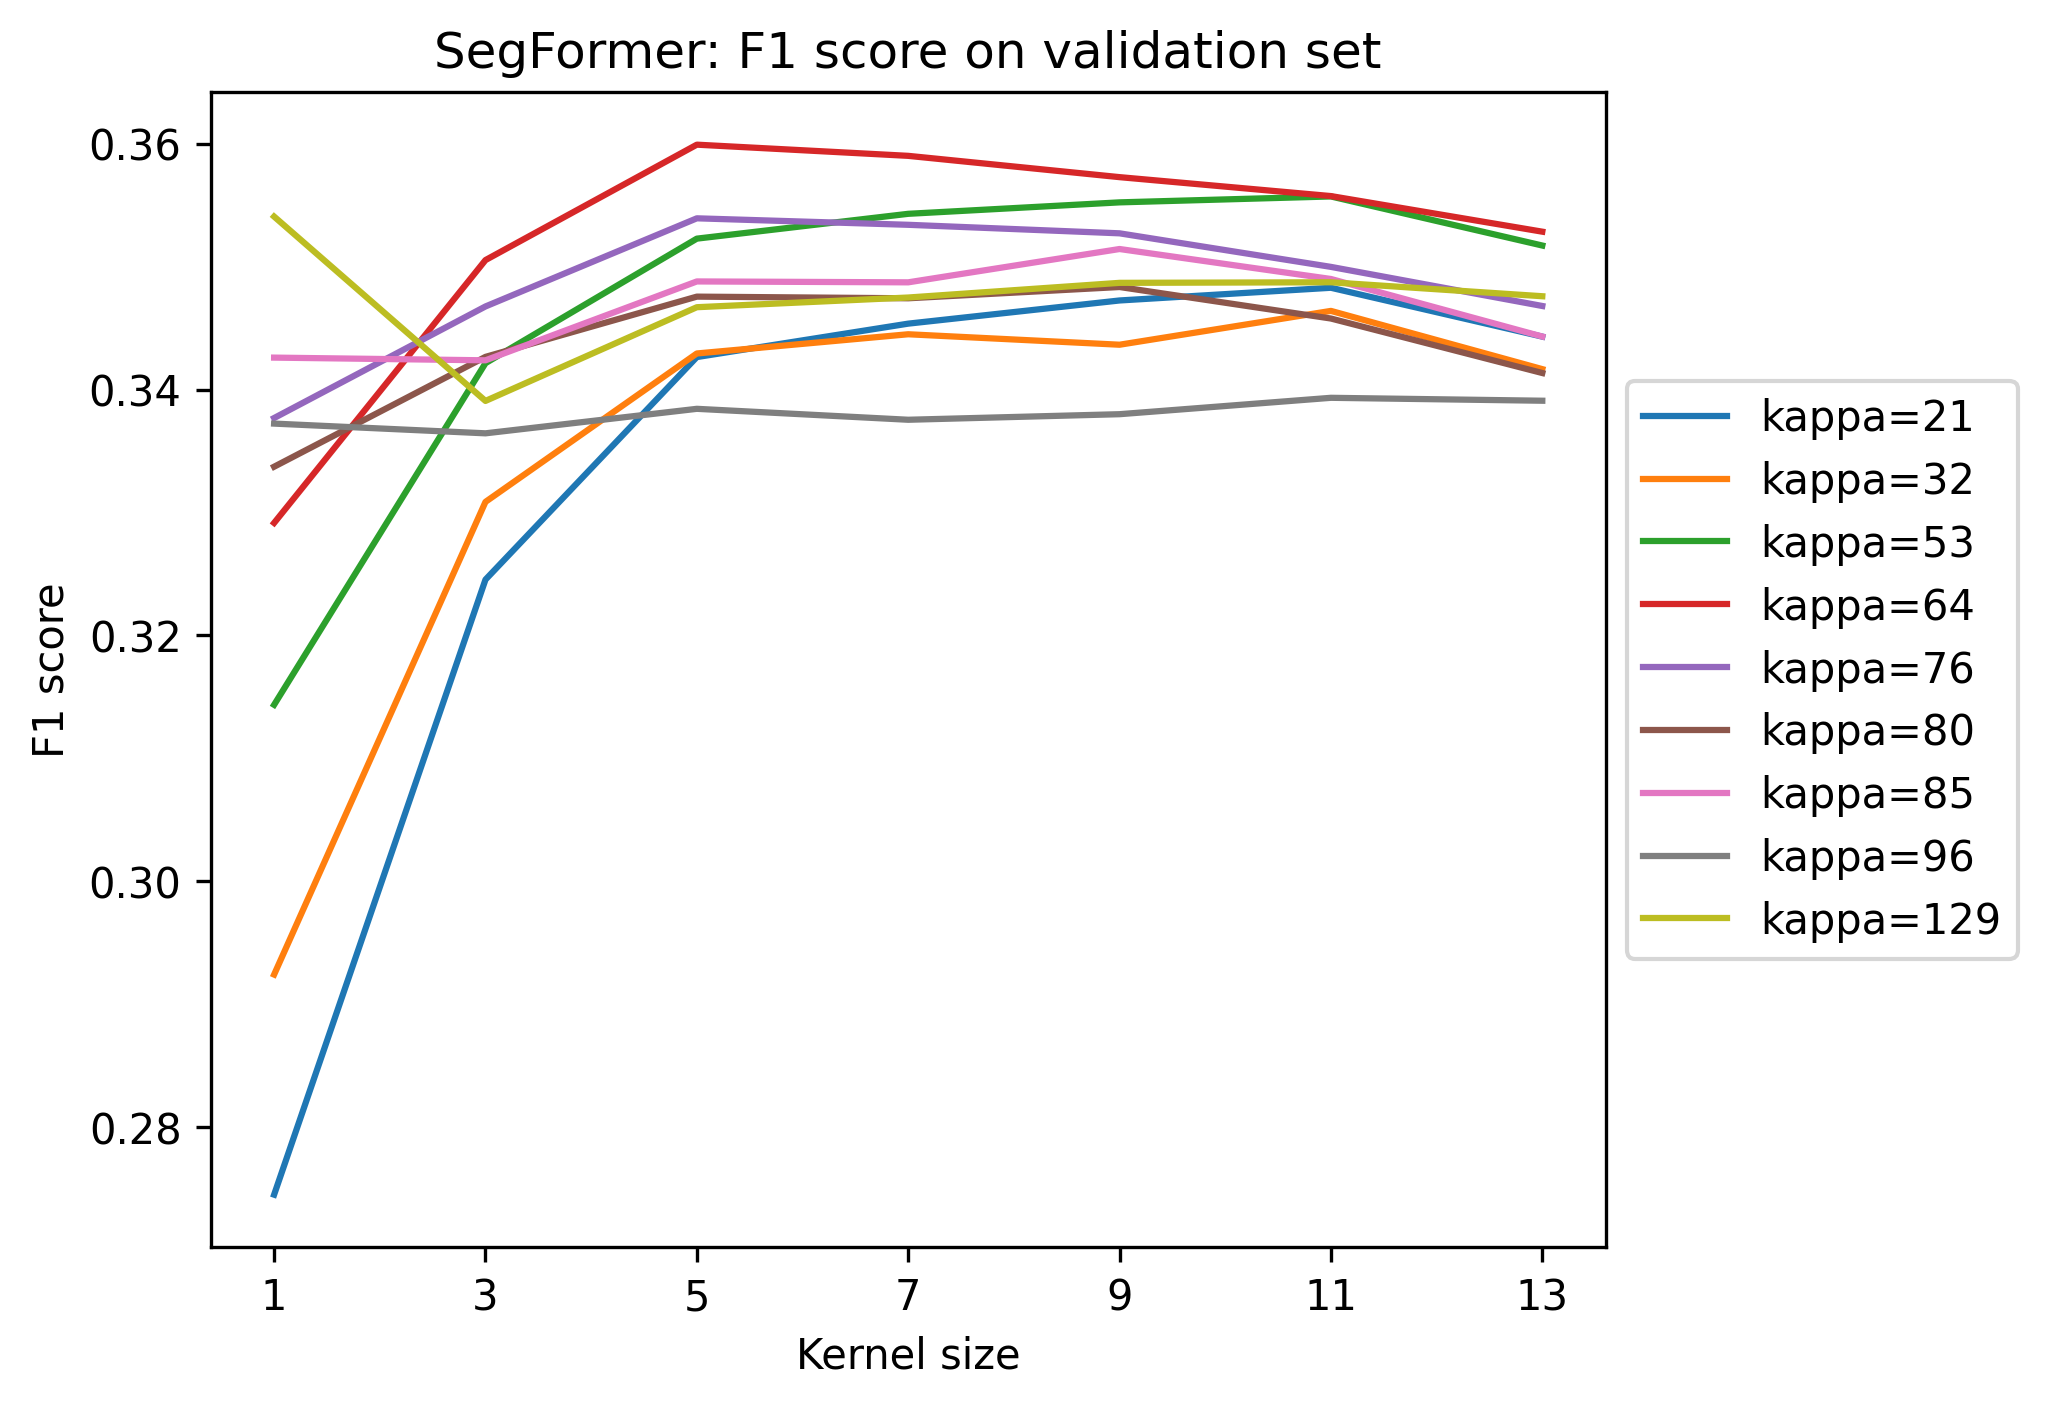
\includegraphics[width=.5\linewidth]{figures/tils/segformer_f1_kappas_kernels_plot.png}
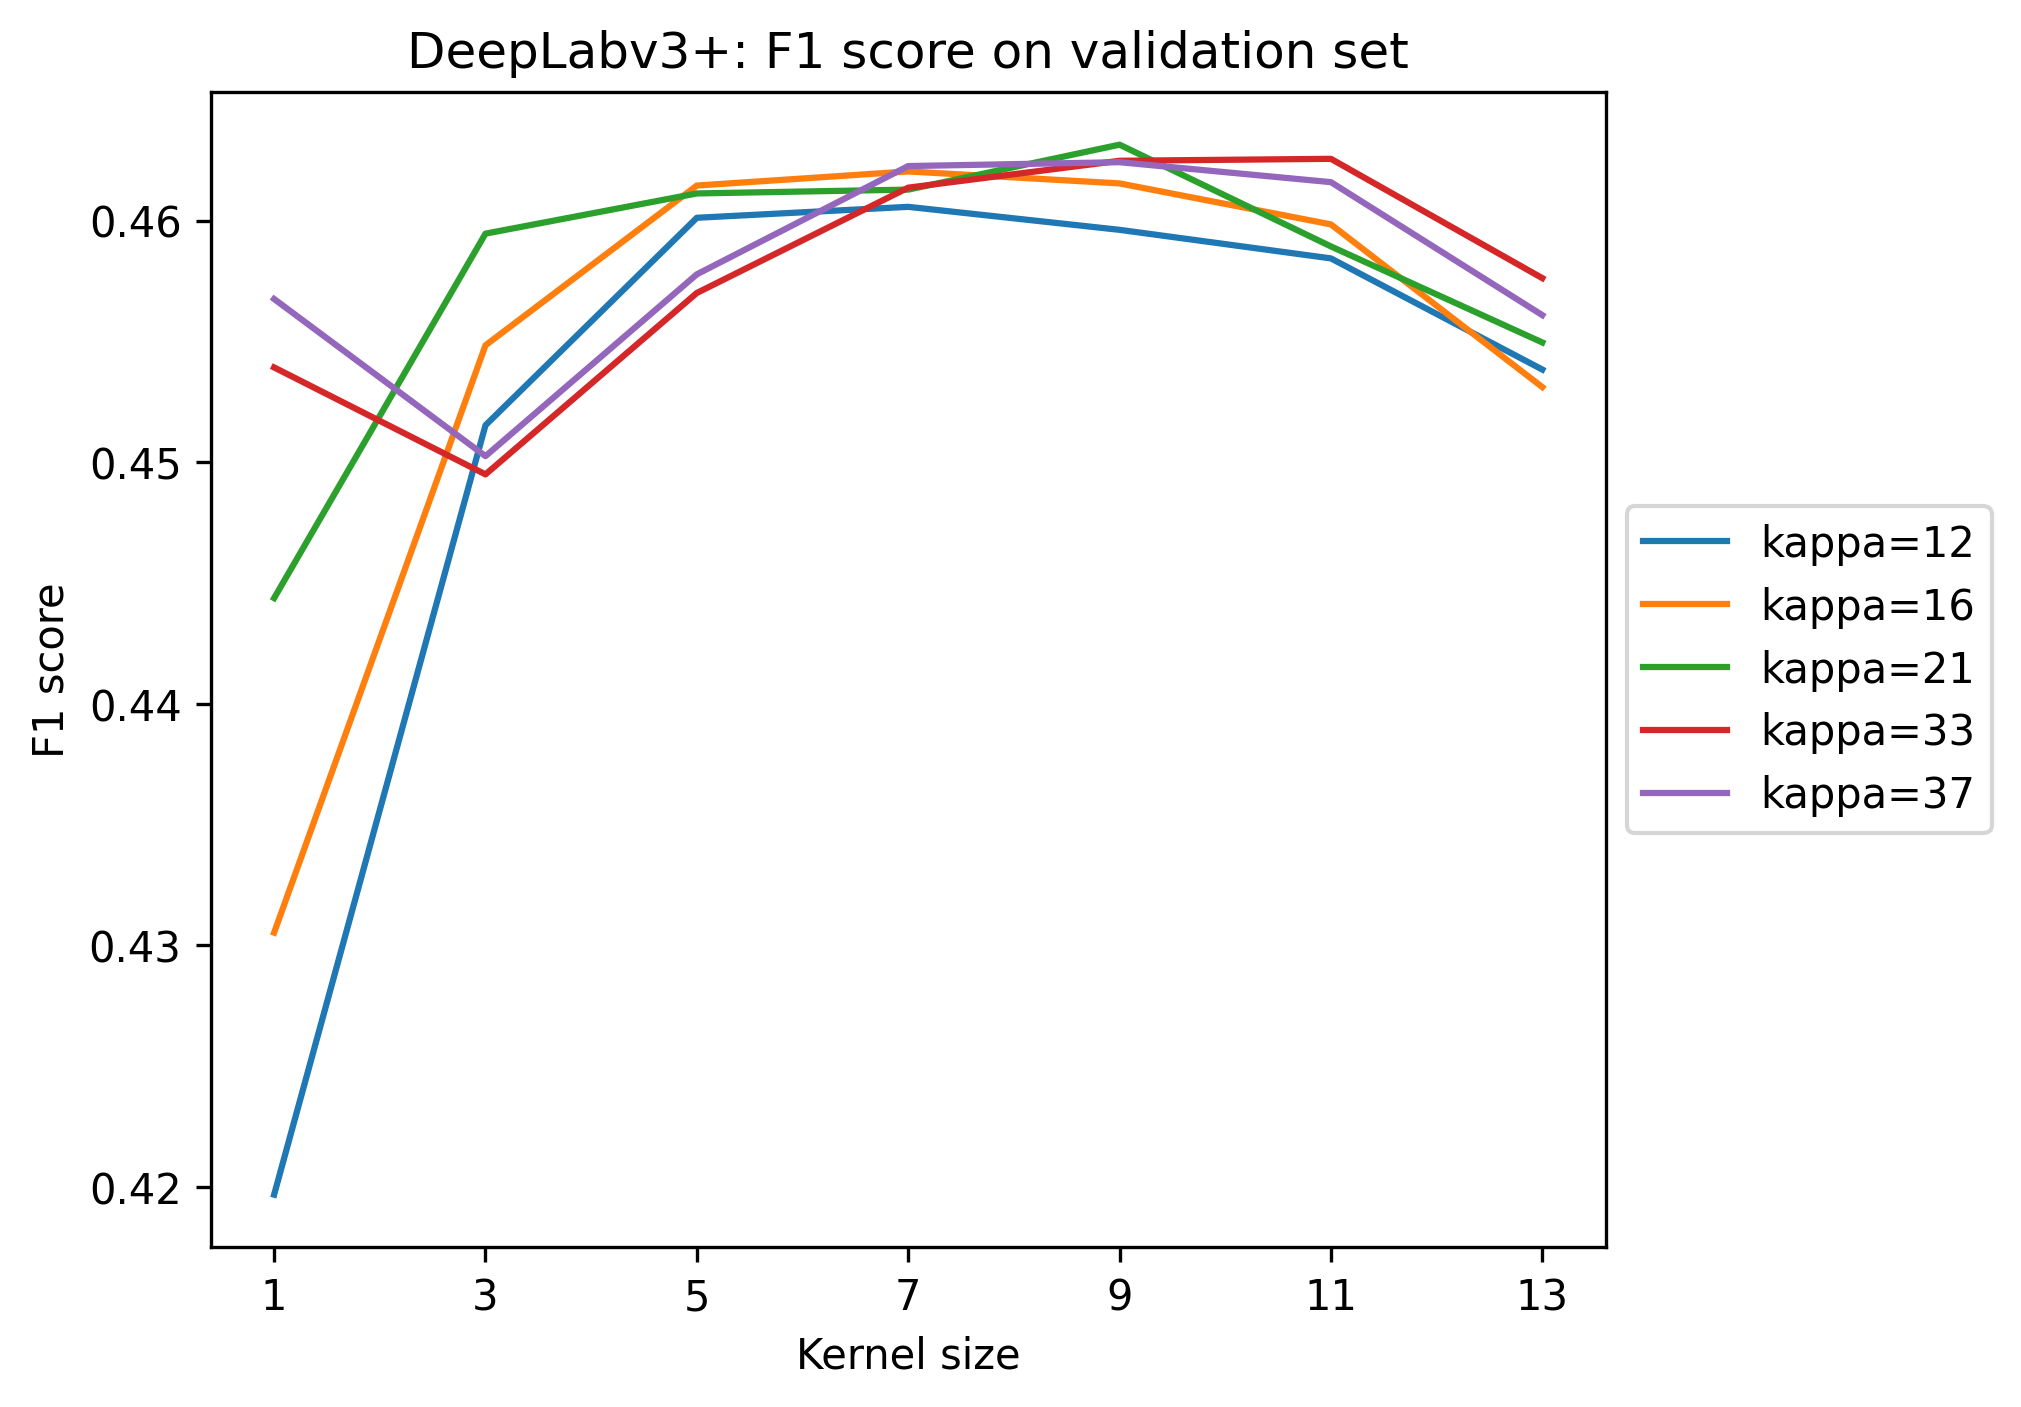
\includegraphics[width=.5\linewidth]{figures/tils/deeplabv3+_f1_kappas_kernels_plot_zooomed.png}
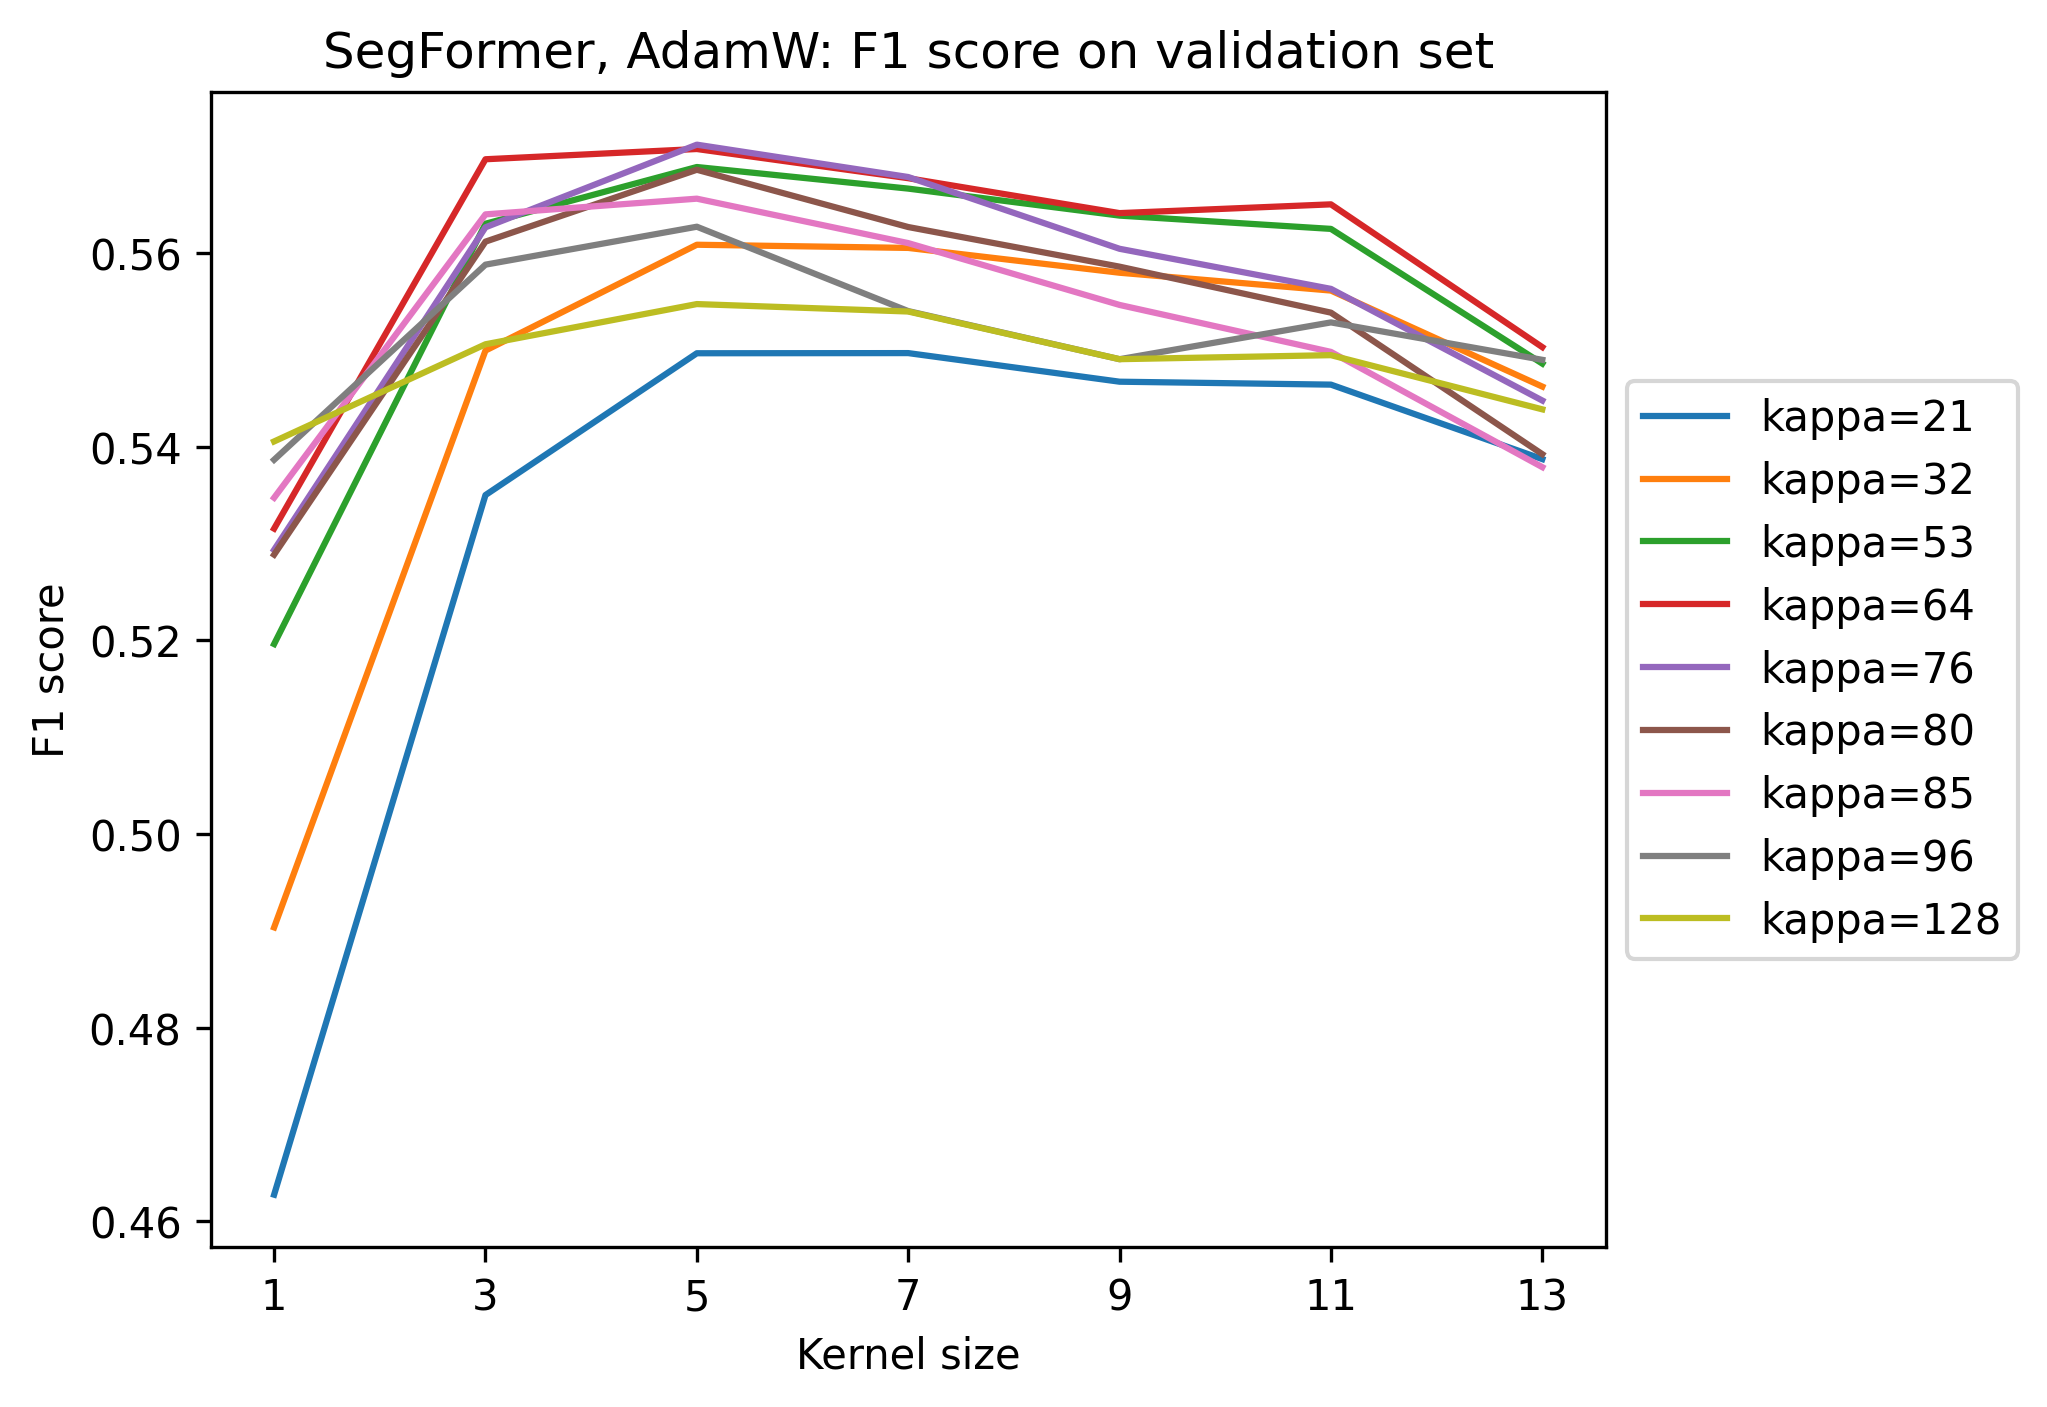
\includegraphics[width=.5\linewidth]{figures/tils/segformer,_adamw_f1_kappas_kernels_plot.png}
\caption{Determination process for best kappa and kernel size for DeepLabv3+
(first in the first row and first in the second row), SegFormer (second in the first row),
and SegFormer with AdamW (second in the second row).}
\label{fig:kappas}
\end{figure}

The final results represented in Table~\ref*{tab:tils_perform} show that SegFormer
model with AdamW optimizer strongly outperforms DeepLabv3+ and simple SegFormer.
Furthermore, while distinguishing the F1 scores between ROIs originating from different medical
centers in Figure~\ref*{fig:tils_dice_boxplots}, SegFormer AdamW results show
significantly better results in all subgroups.
\begin{figure}[H]
    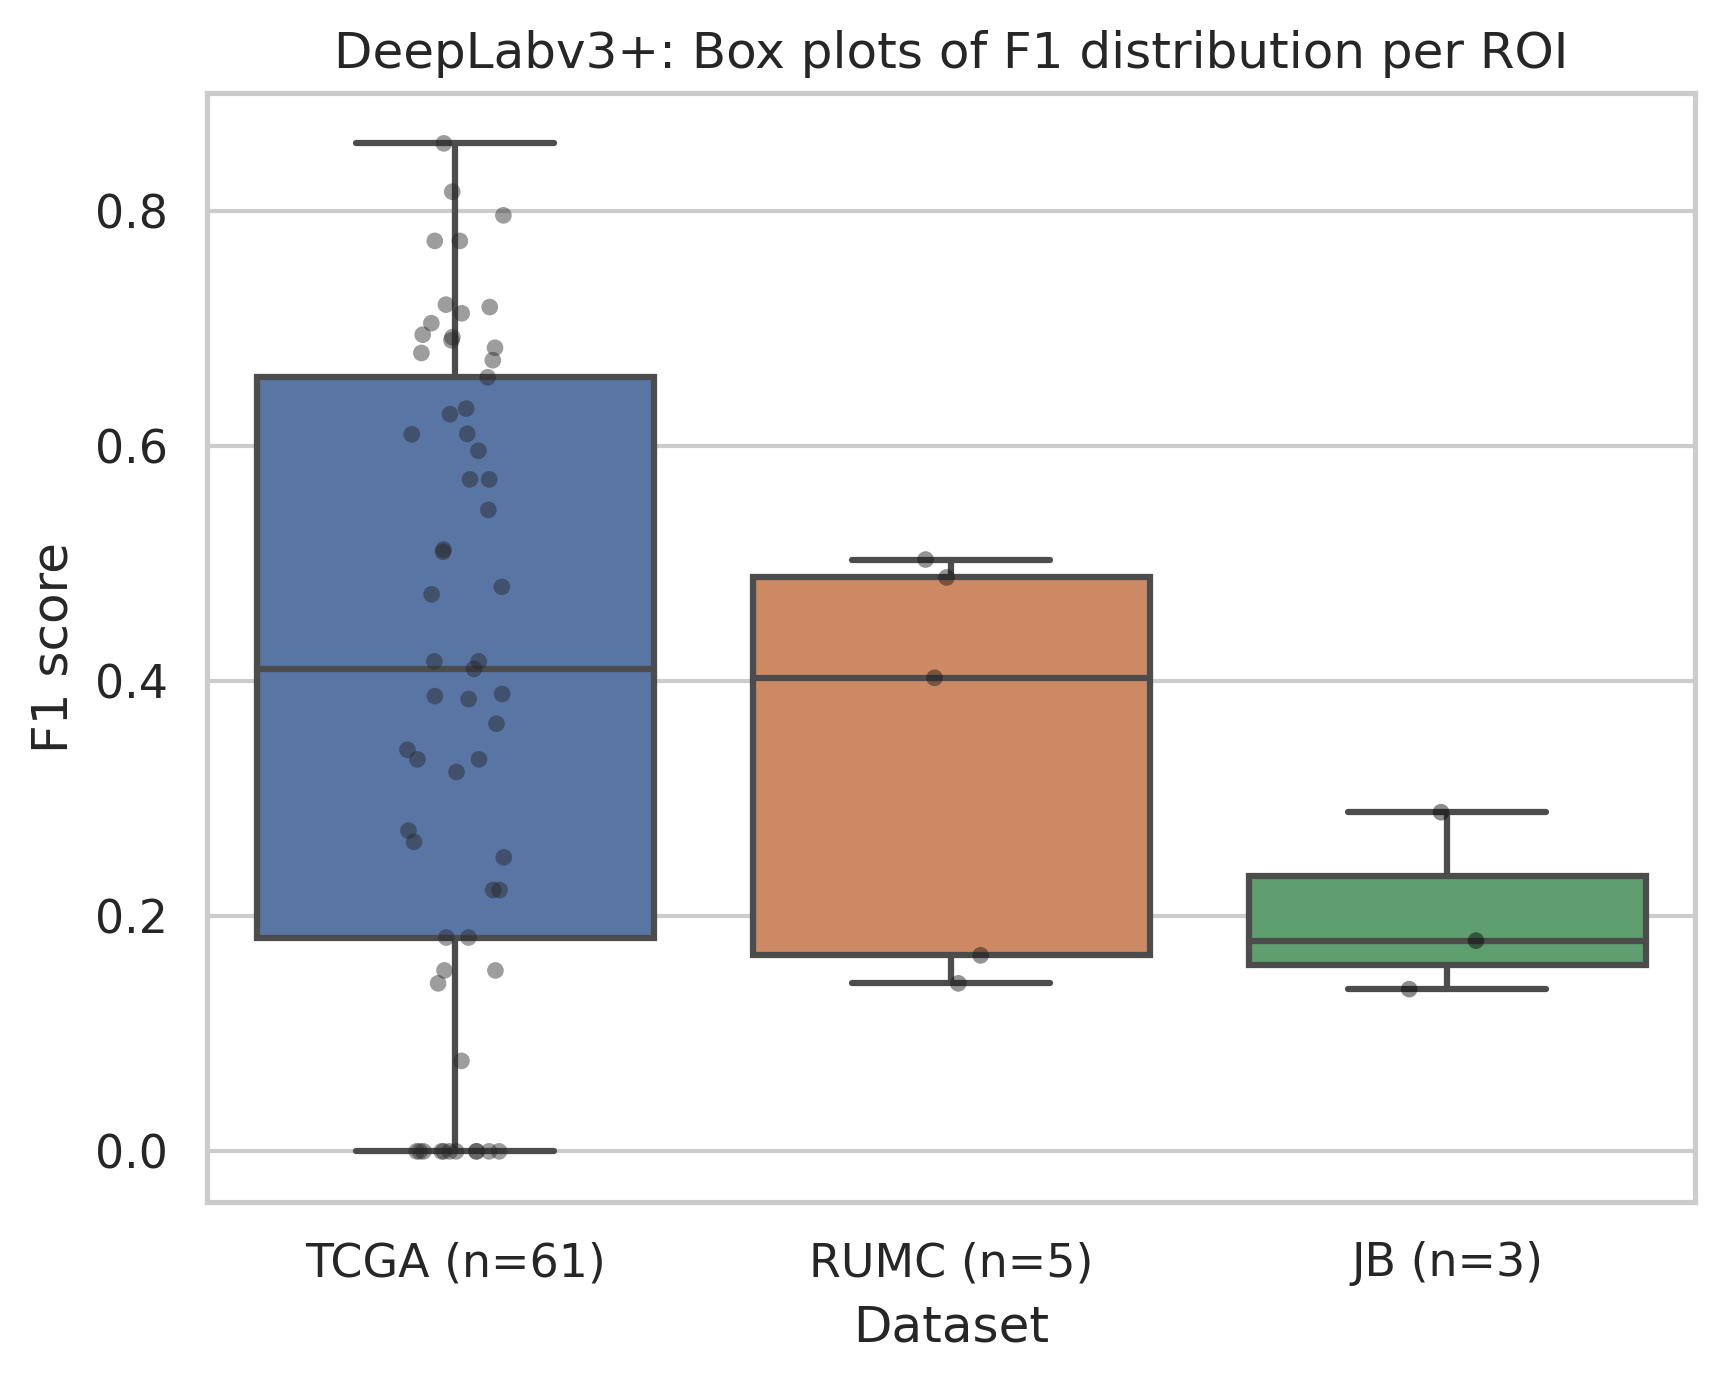
\includegraphics[width=.32\linewidth]{figures/tils/deeplabv3+_F1_roi_adj.png}
    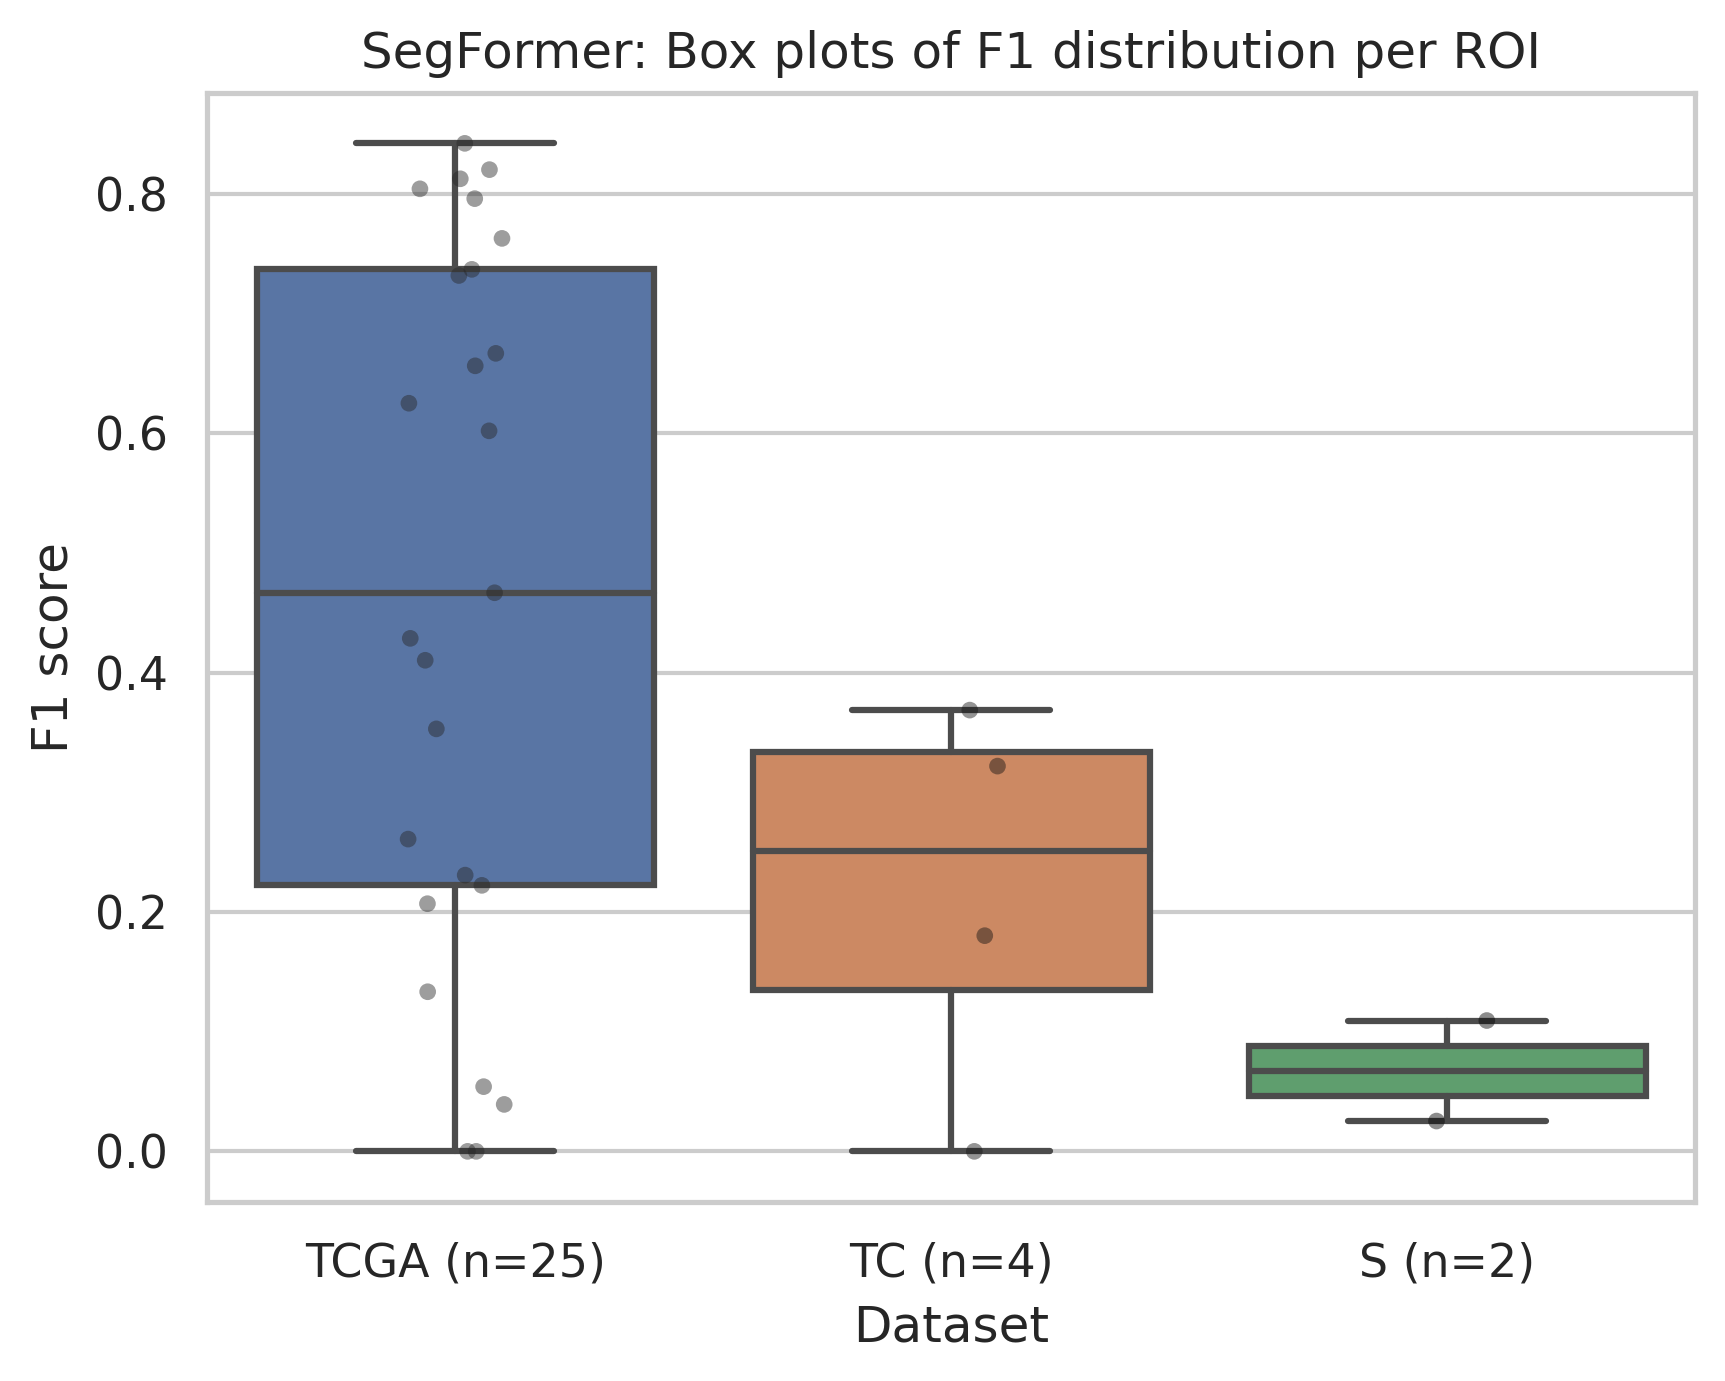
\includegraphics[width=.32\linewidth]{figures/tils/segformer_F1_roi_adj.png}
    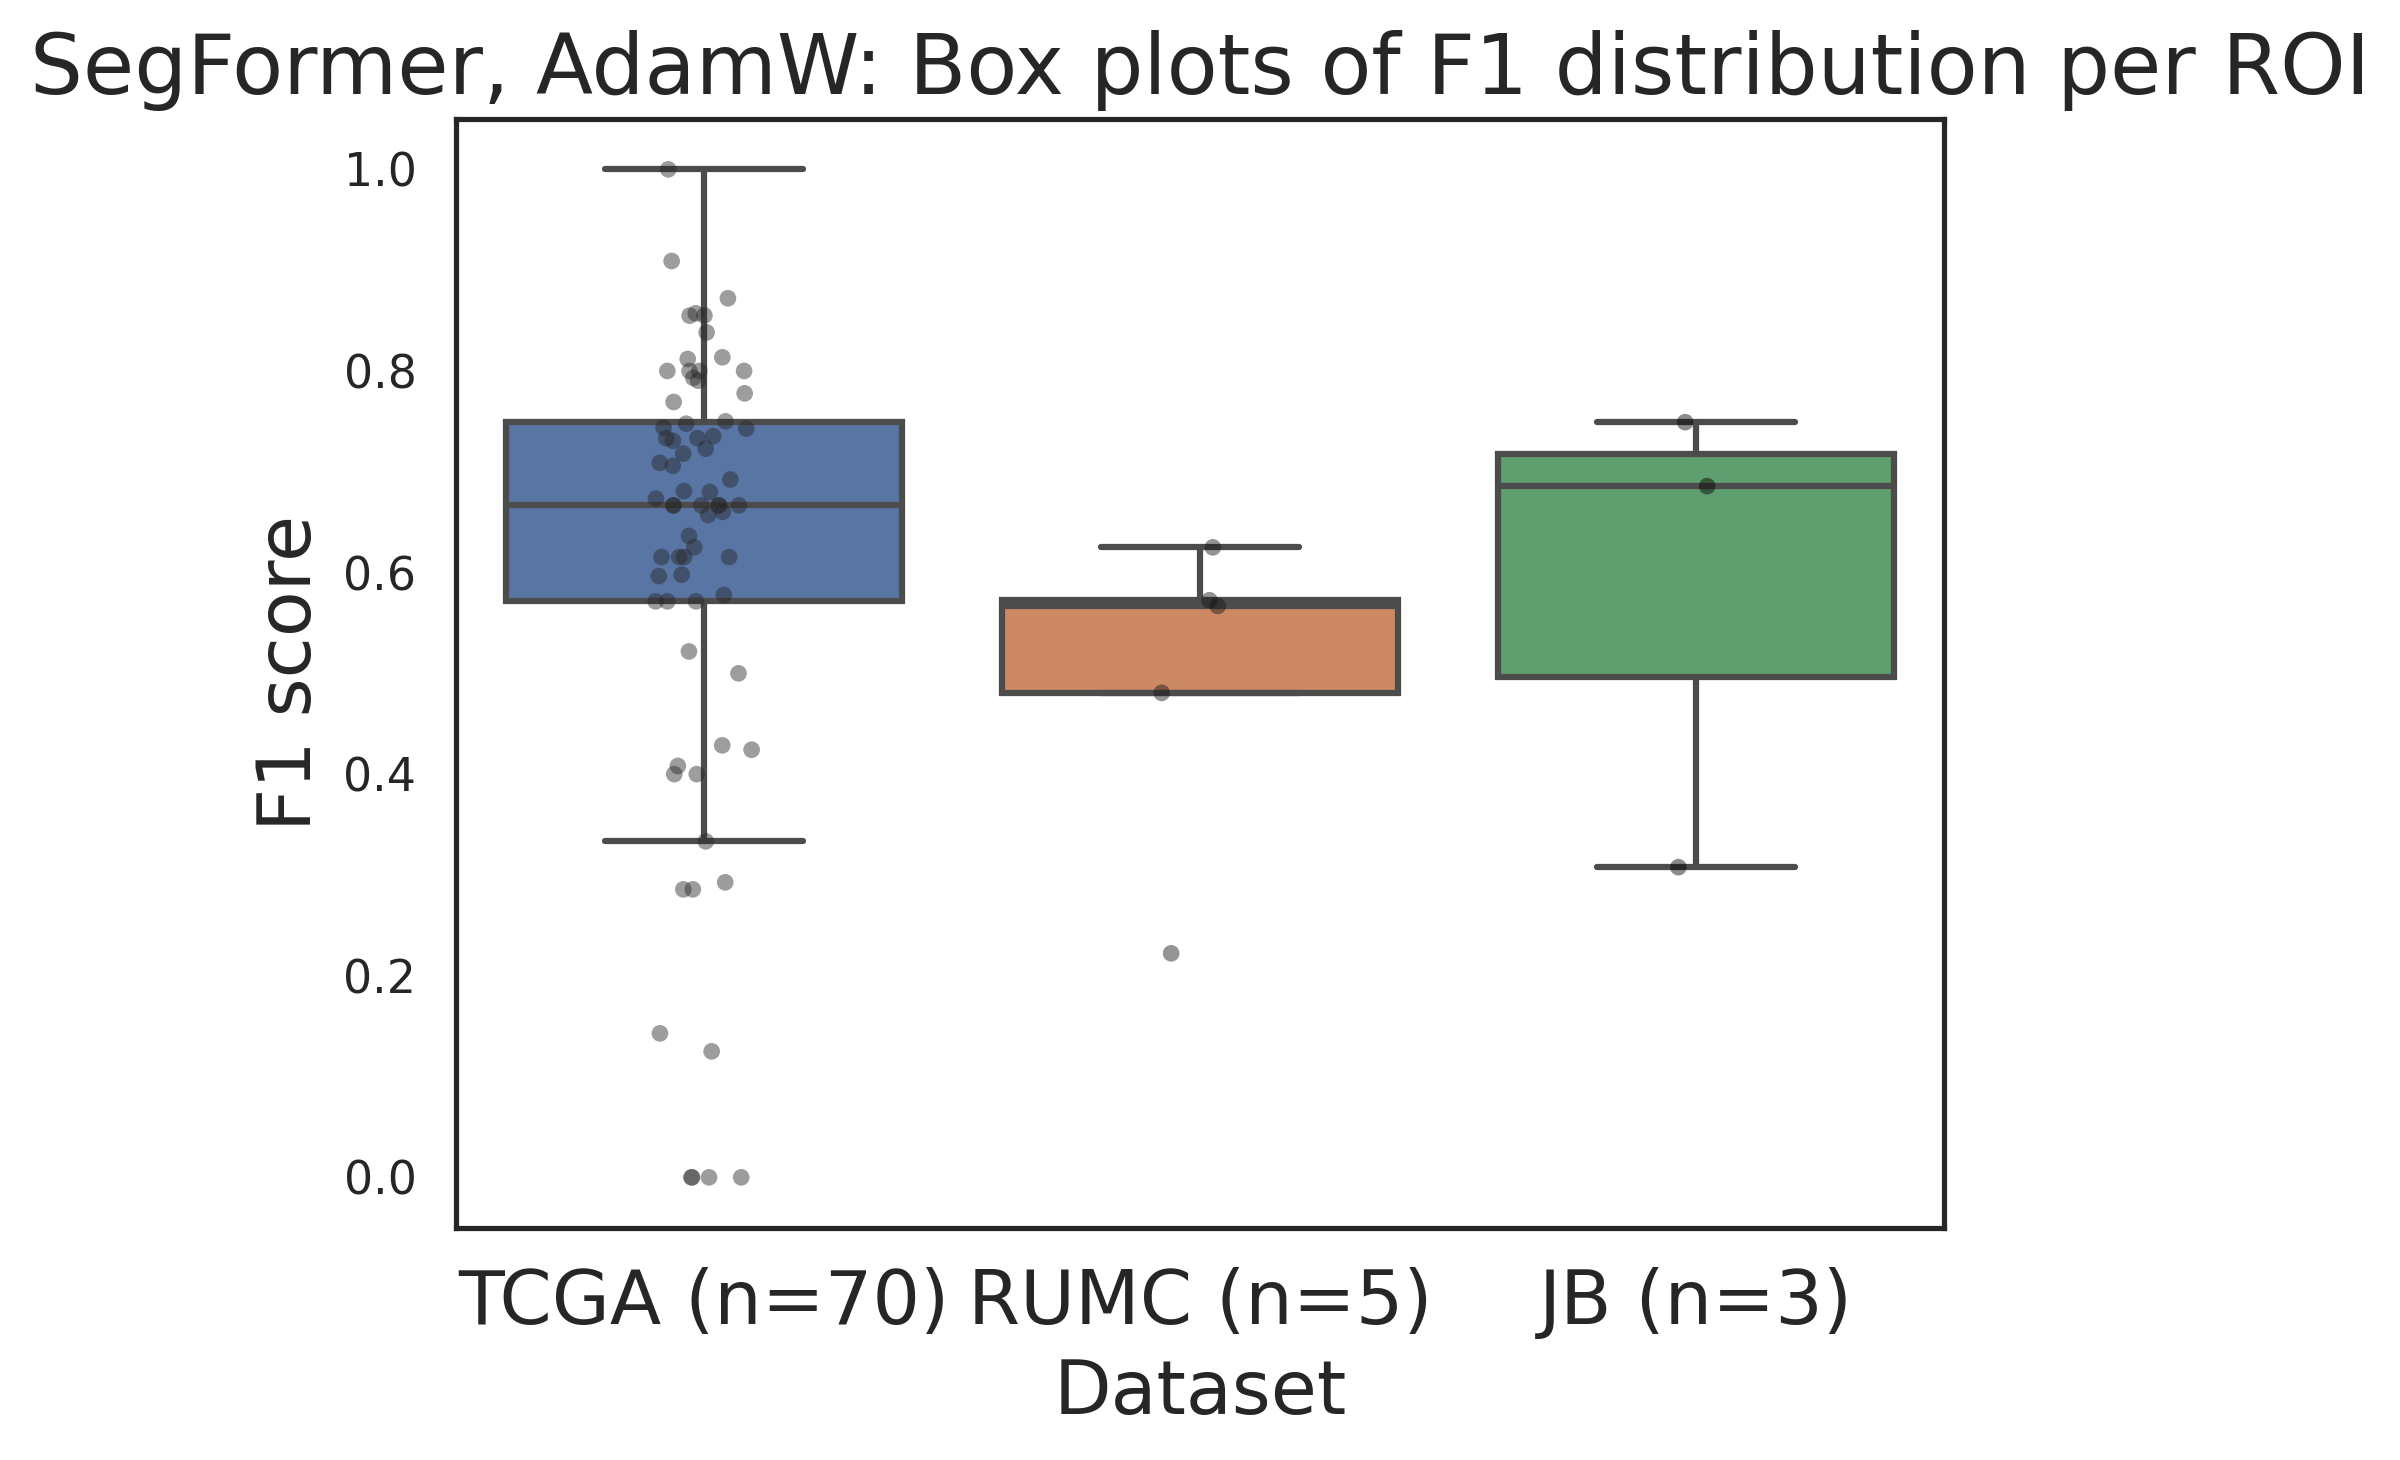
\includegraphics[width=.32\linewidth]{figures/tils/segformer,_adamw_F1_roi_adj.png}
    \caption{Boxplots of dice score across three datastes (TCGA-BRCA, RUMC, JB) with
    maximum allowed distance between ground truth and prediction equals 10 pixels (5 \textmu m).}
    \label{fig:tils_dice_boxplots}
\end{figure}
Interestingly the precision boxplots
in Figure~\ref*{fig:tils_pr_r_boxplots} do not show such an unequivocal superiority,
where in the JB subgroup simple SegFormer manages to predict fewer false positives and 
(n=2) indicates that the model managed to predict empty ROI as a complete rest region,
which is not the case for any other model.
In more detailed
Figure~\ref*{fig:TCGA-D8-A142_tils} one can see the intermediate steps of
how the posteriors are simplified into point segmentations and later the misted,
falsely annotated and correct TILs can be compared. Even on the level of posteriors
(overlayed with H\&E image), it is visible that SegFormer AdamW manages to detect
more regions, especially closer to the border of the image. The grids in Figure~\ref*{fig:TCGA-D8-A142_tils}
were added for readers' convenience and are not artifacts. 

\begin{figure}[H]
    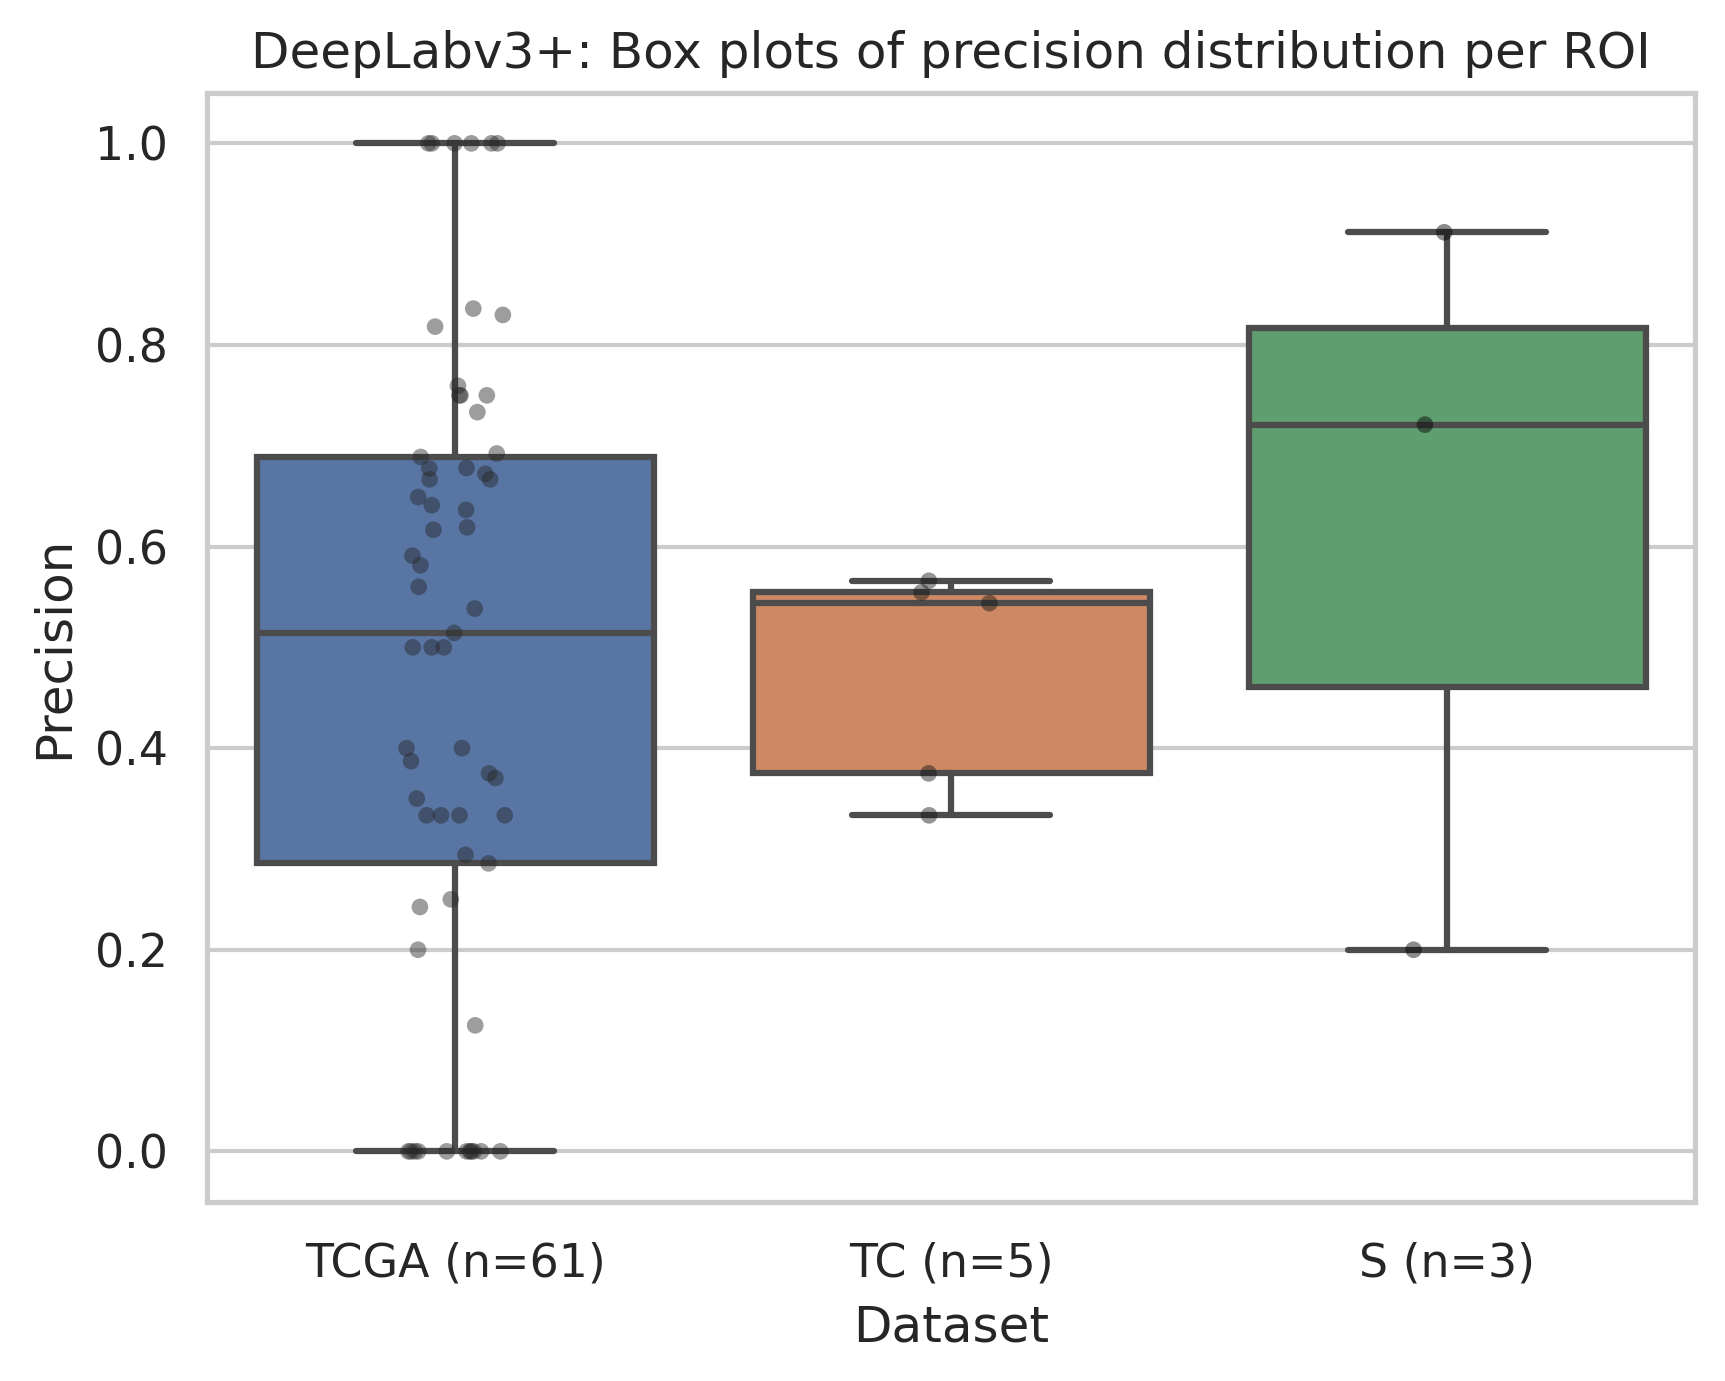
\includegraphics[width=.32\linewidth]{figures/tils/deeplabv3+_precision_roi_adj.png}
    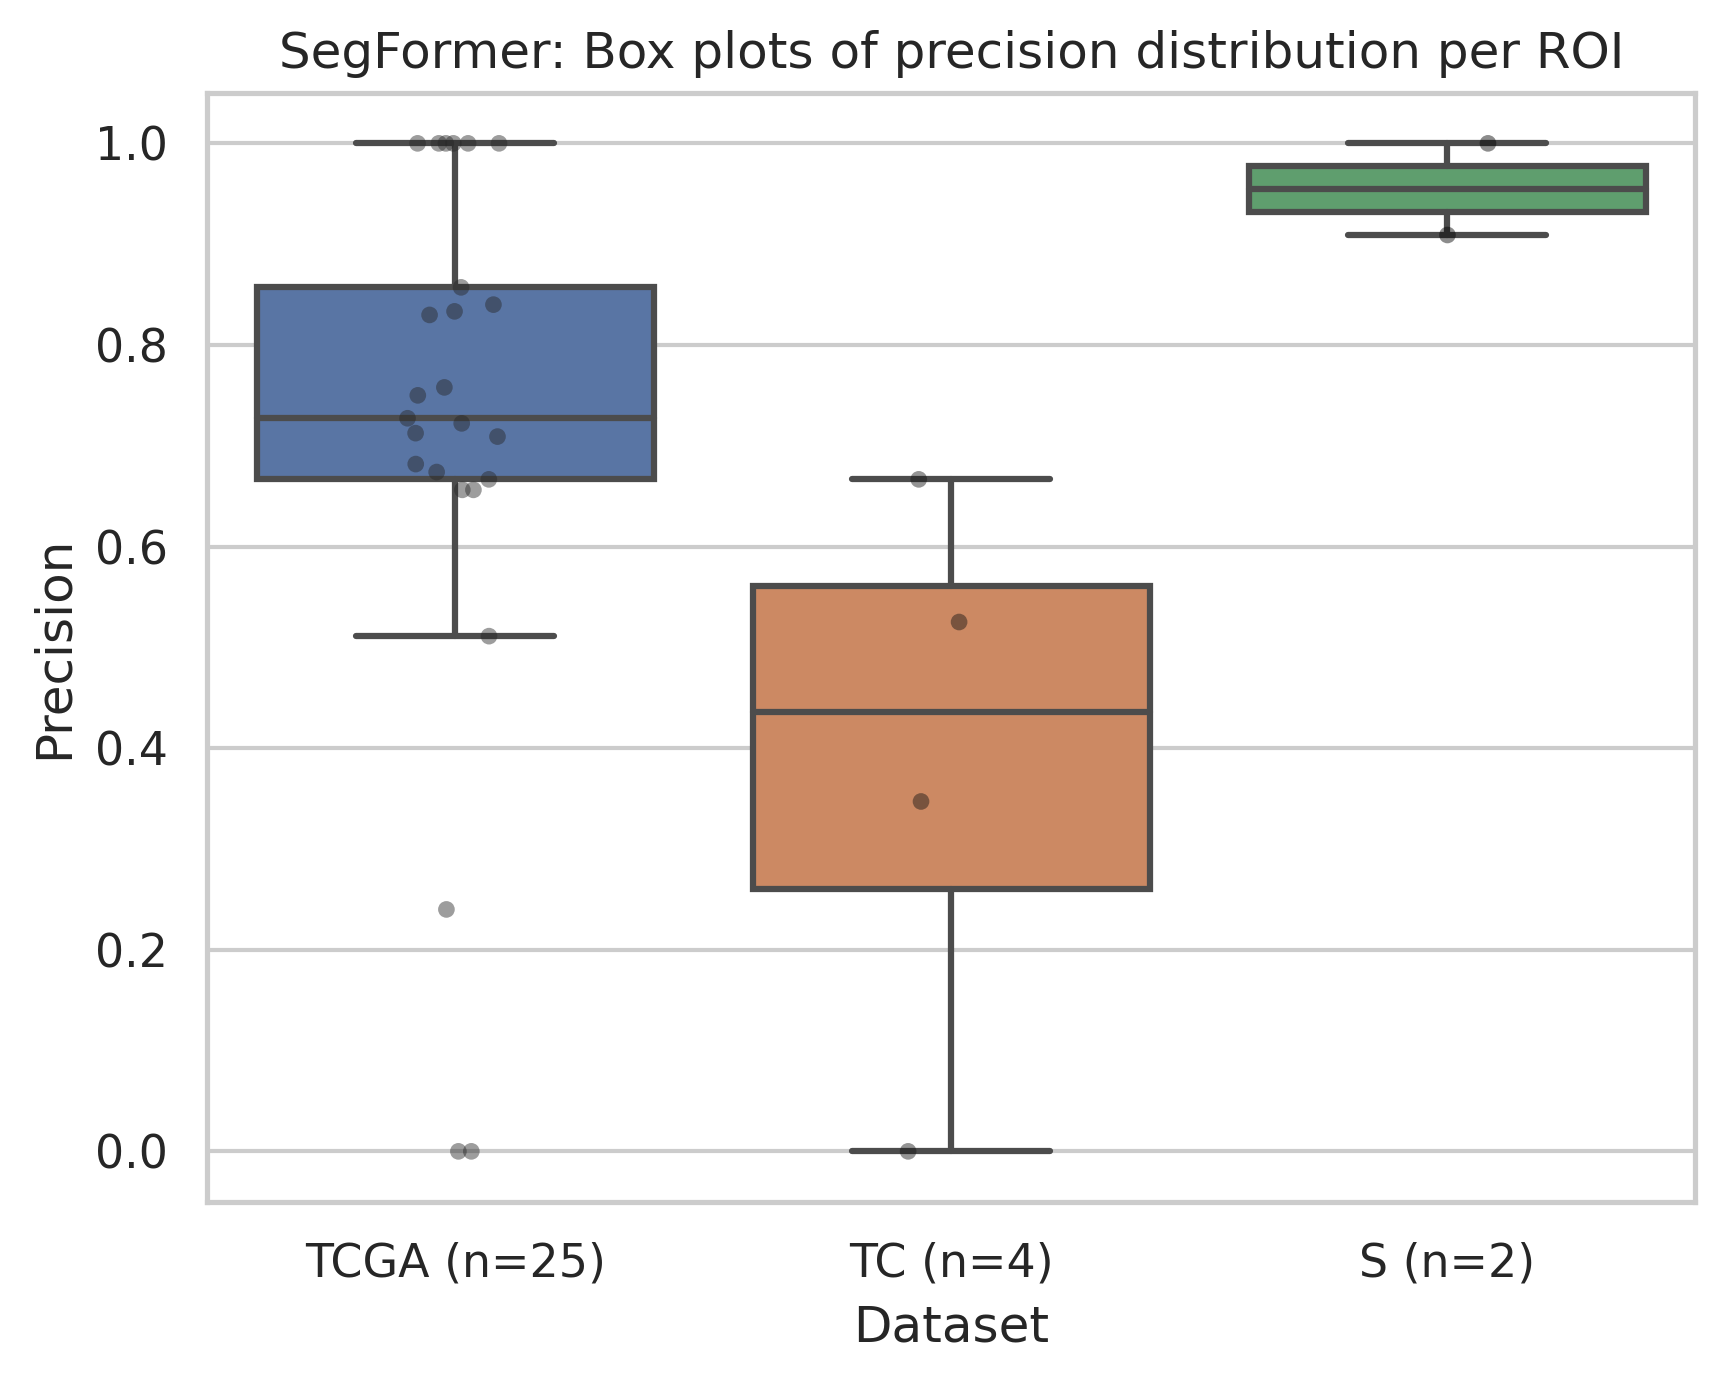
\includegraphics[width=.32\linewidth]{figures/tils/segformer_precision_roi_adj.png}
    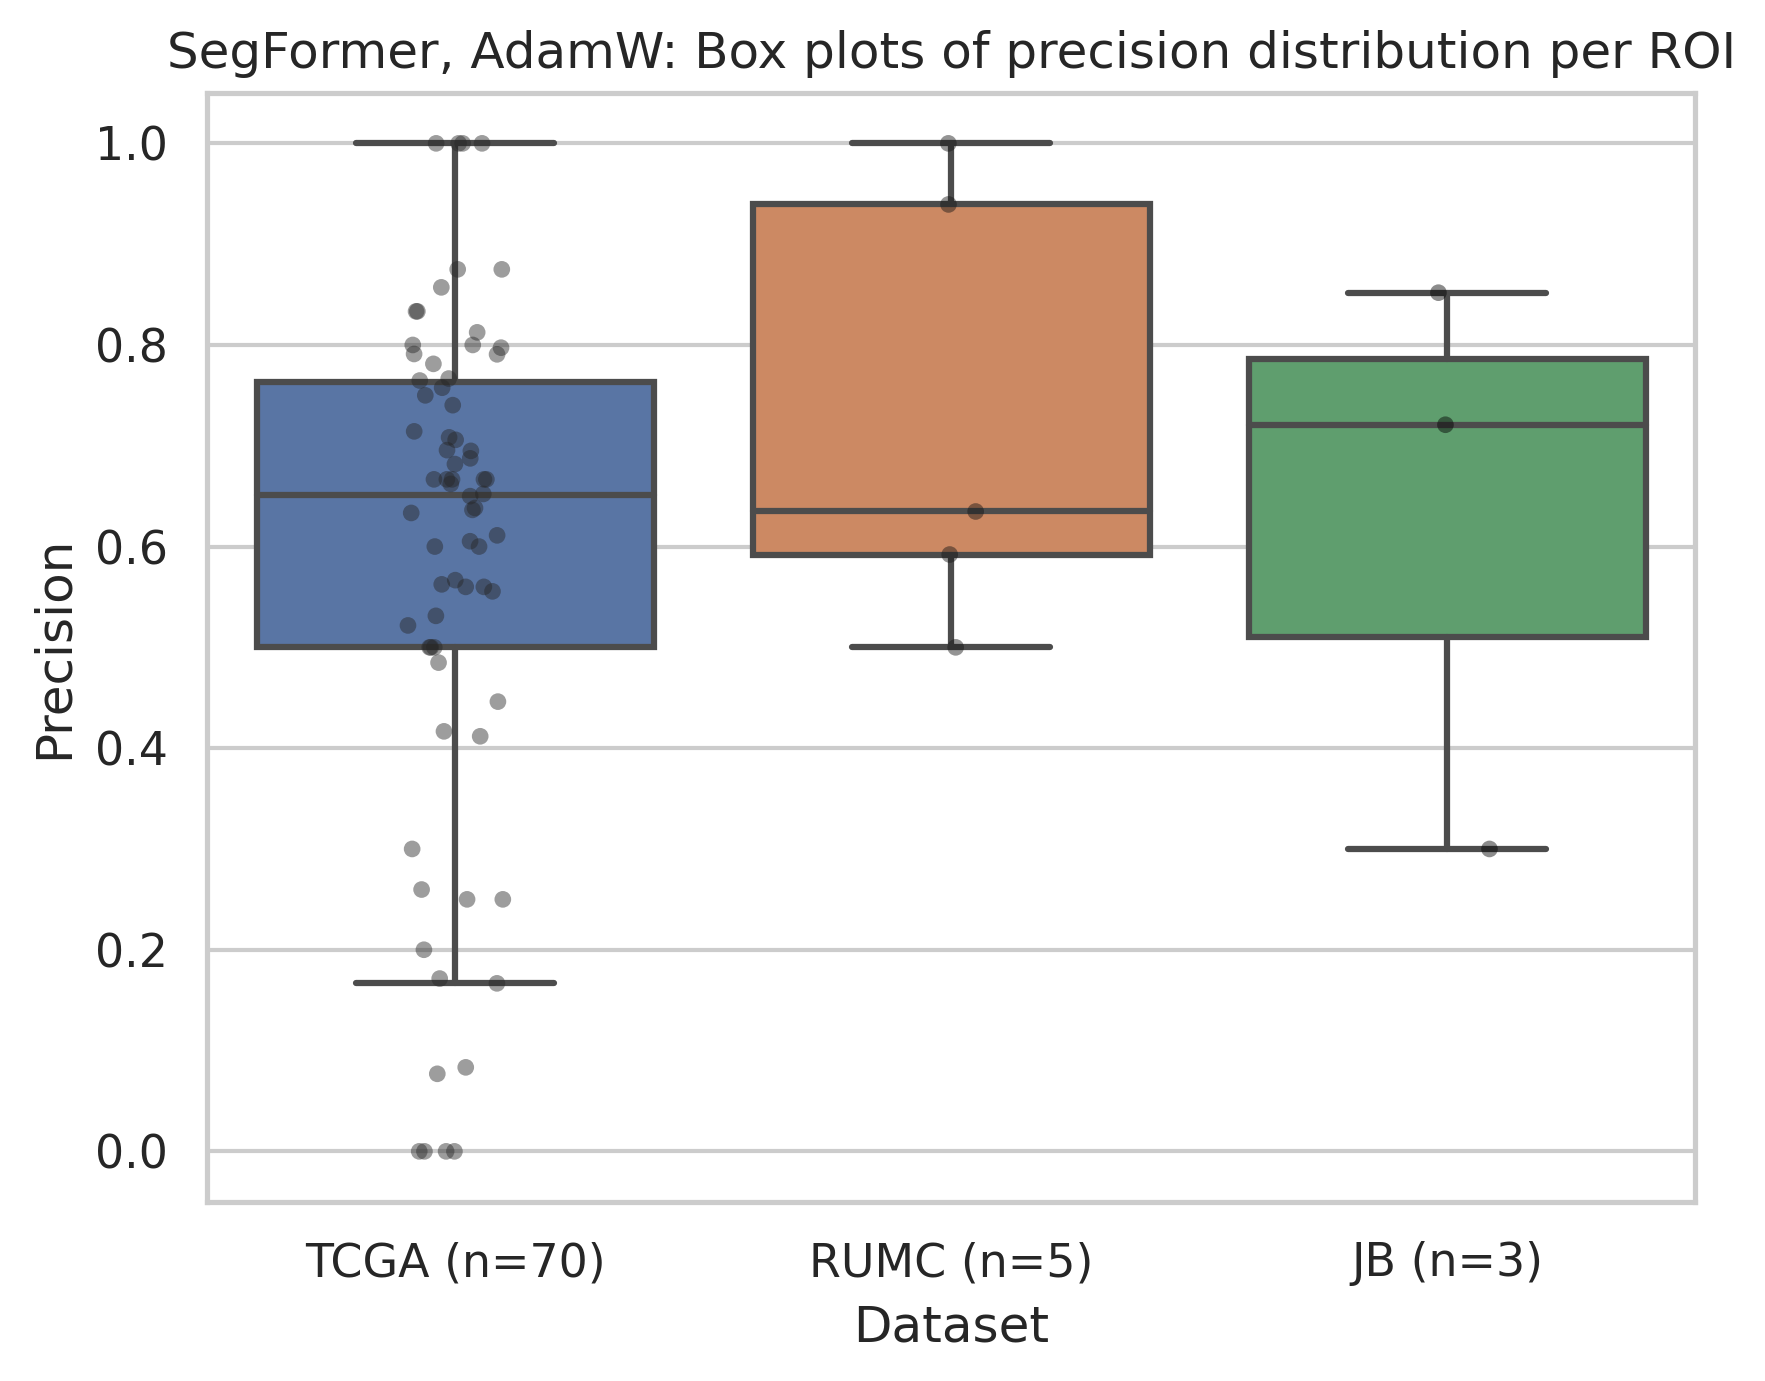
\includegraphics[width=.32\linewidth]{figures/tils/segformer,_adamw_precision_roi_adj.png}
    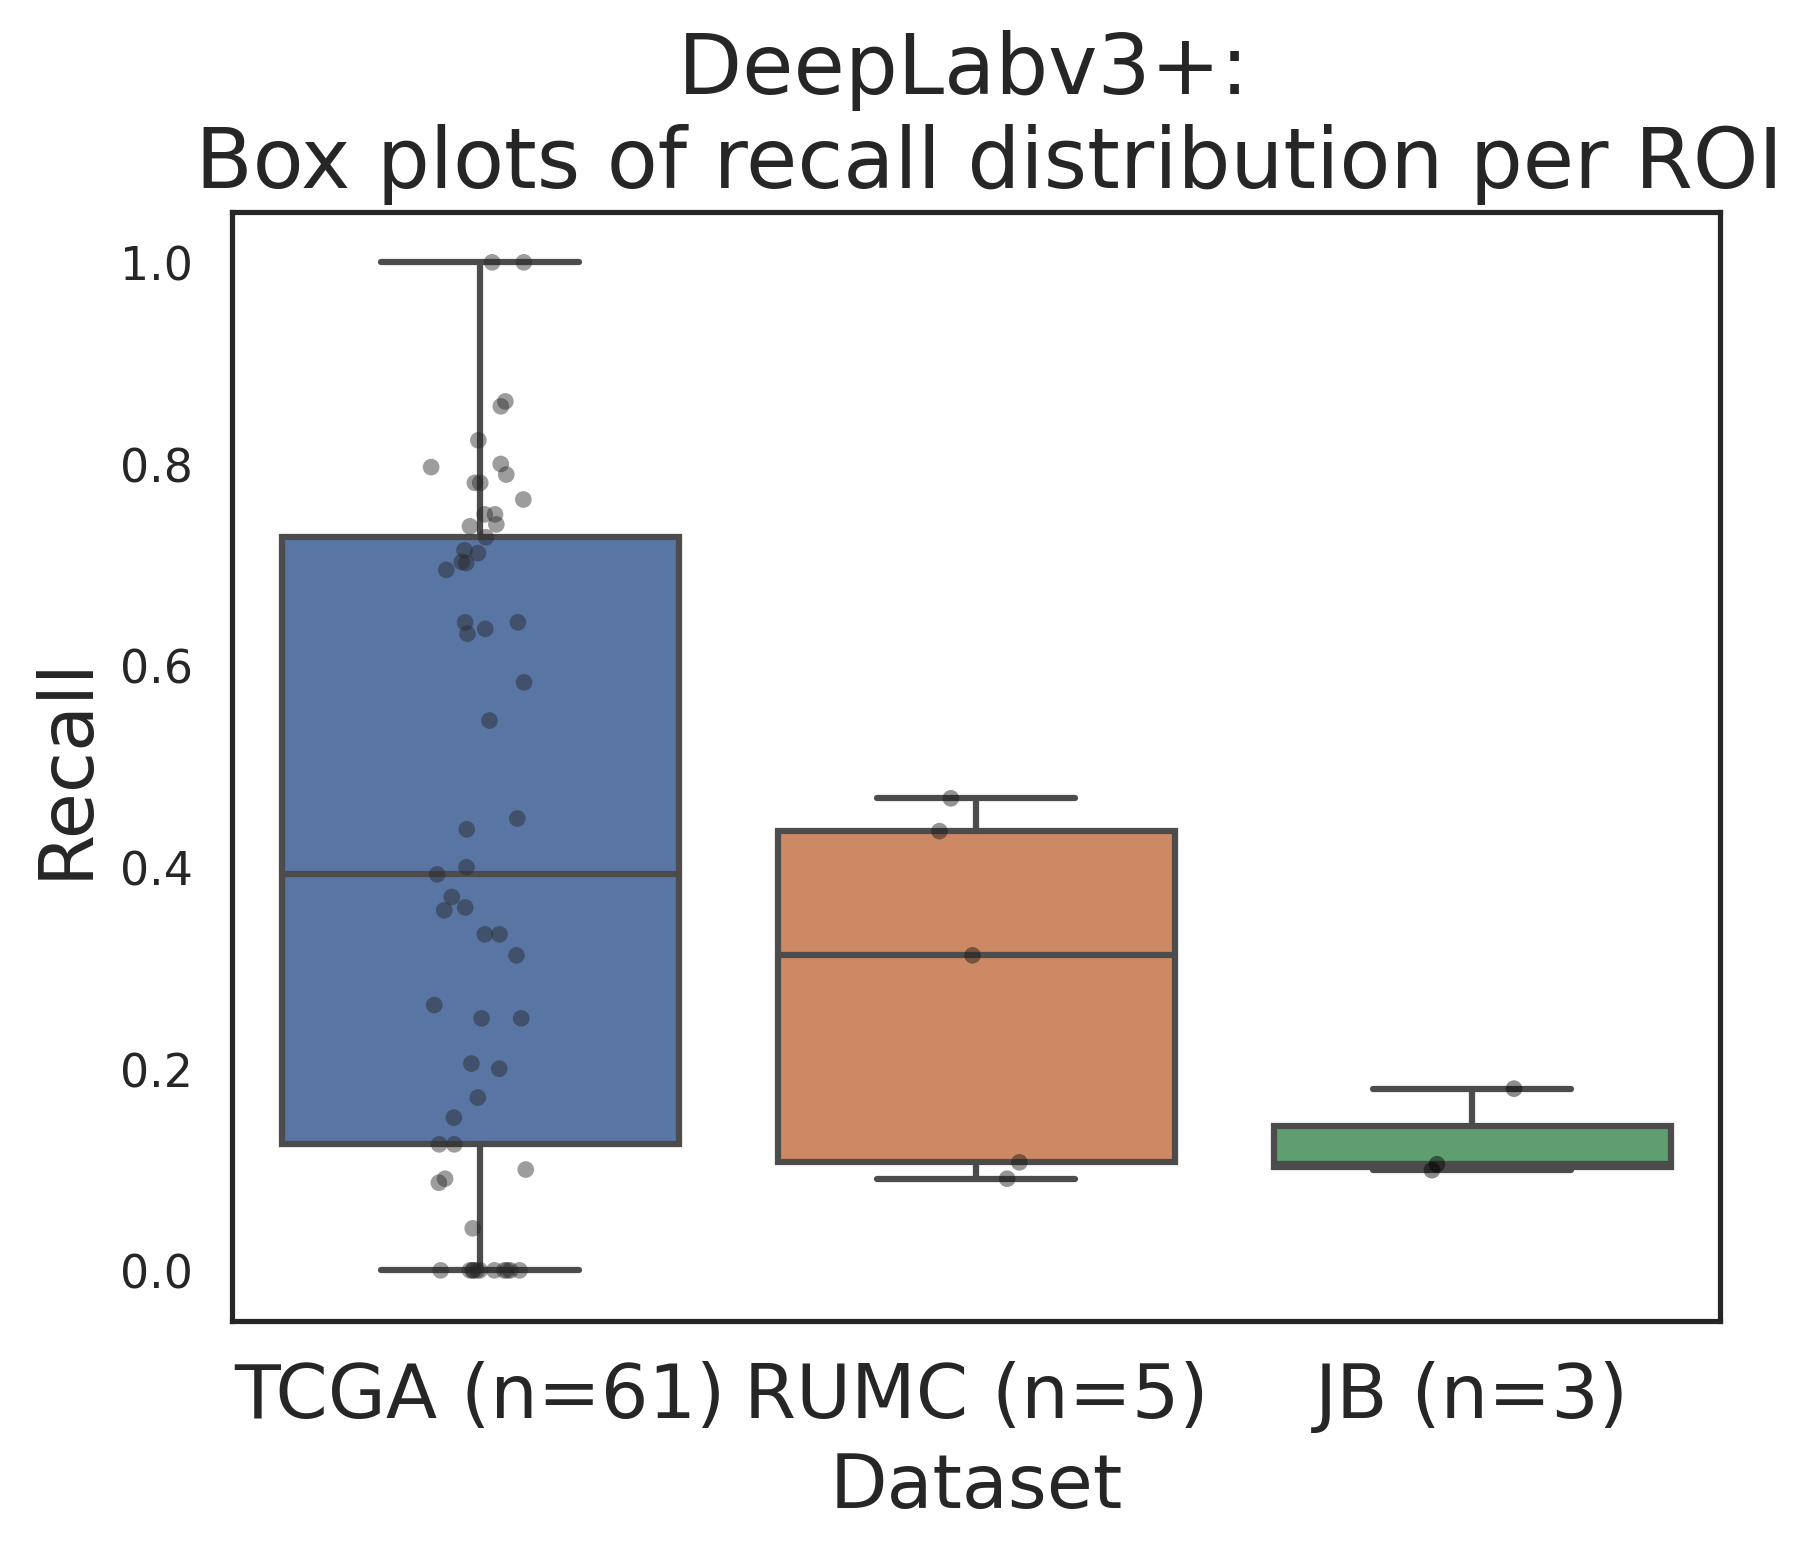
\includegraphics[width=.32\linewidth]{figures/tils/deeplabv3+_recall_roi_adj.png}
    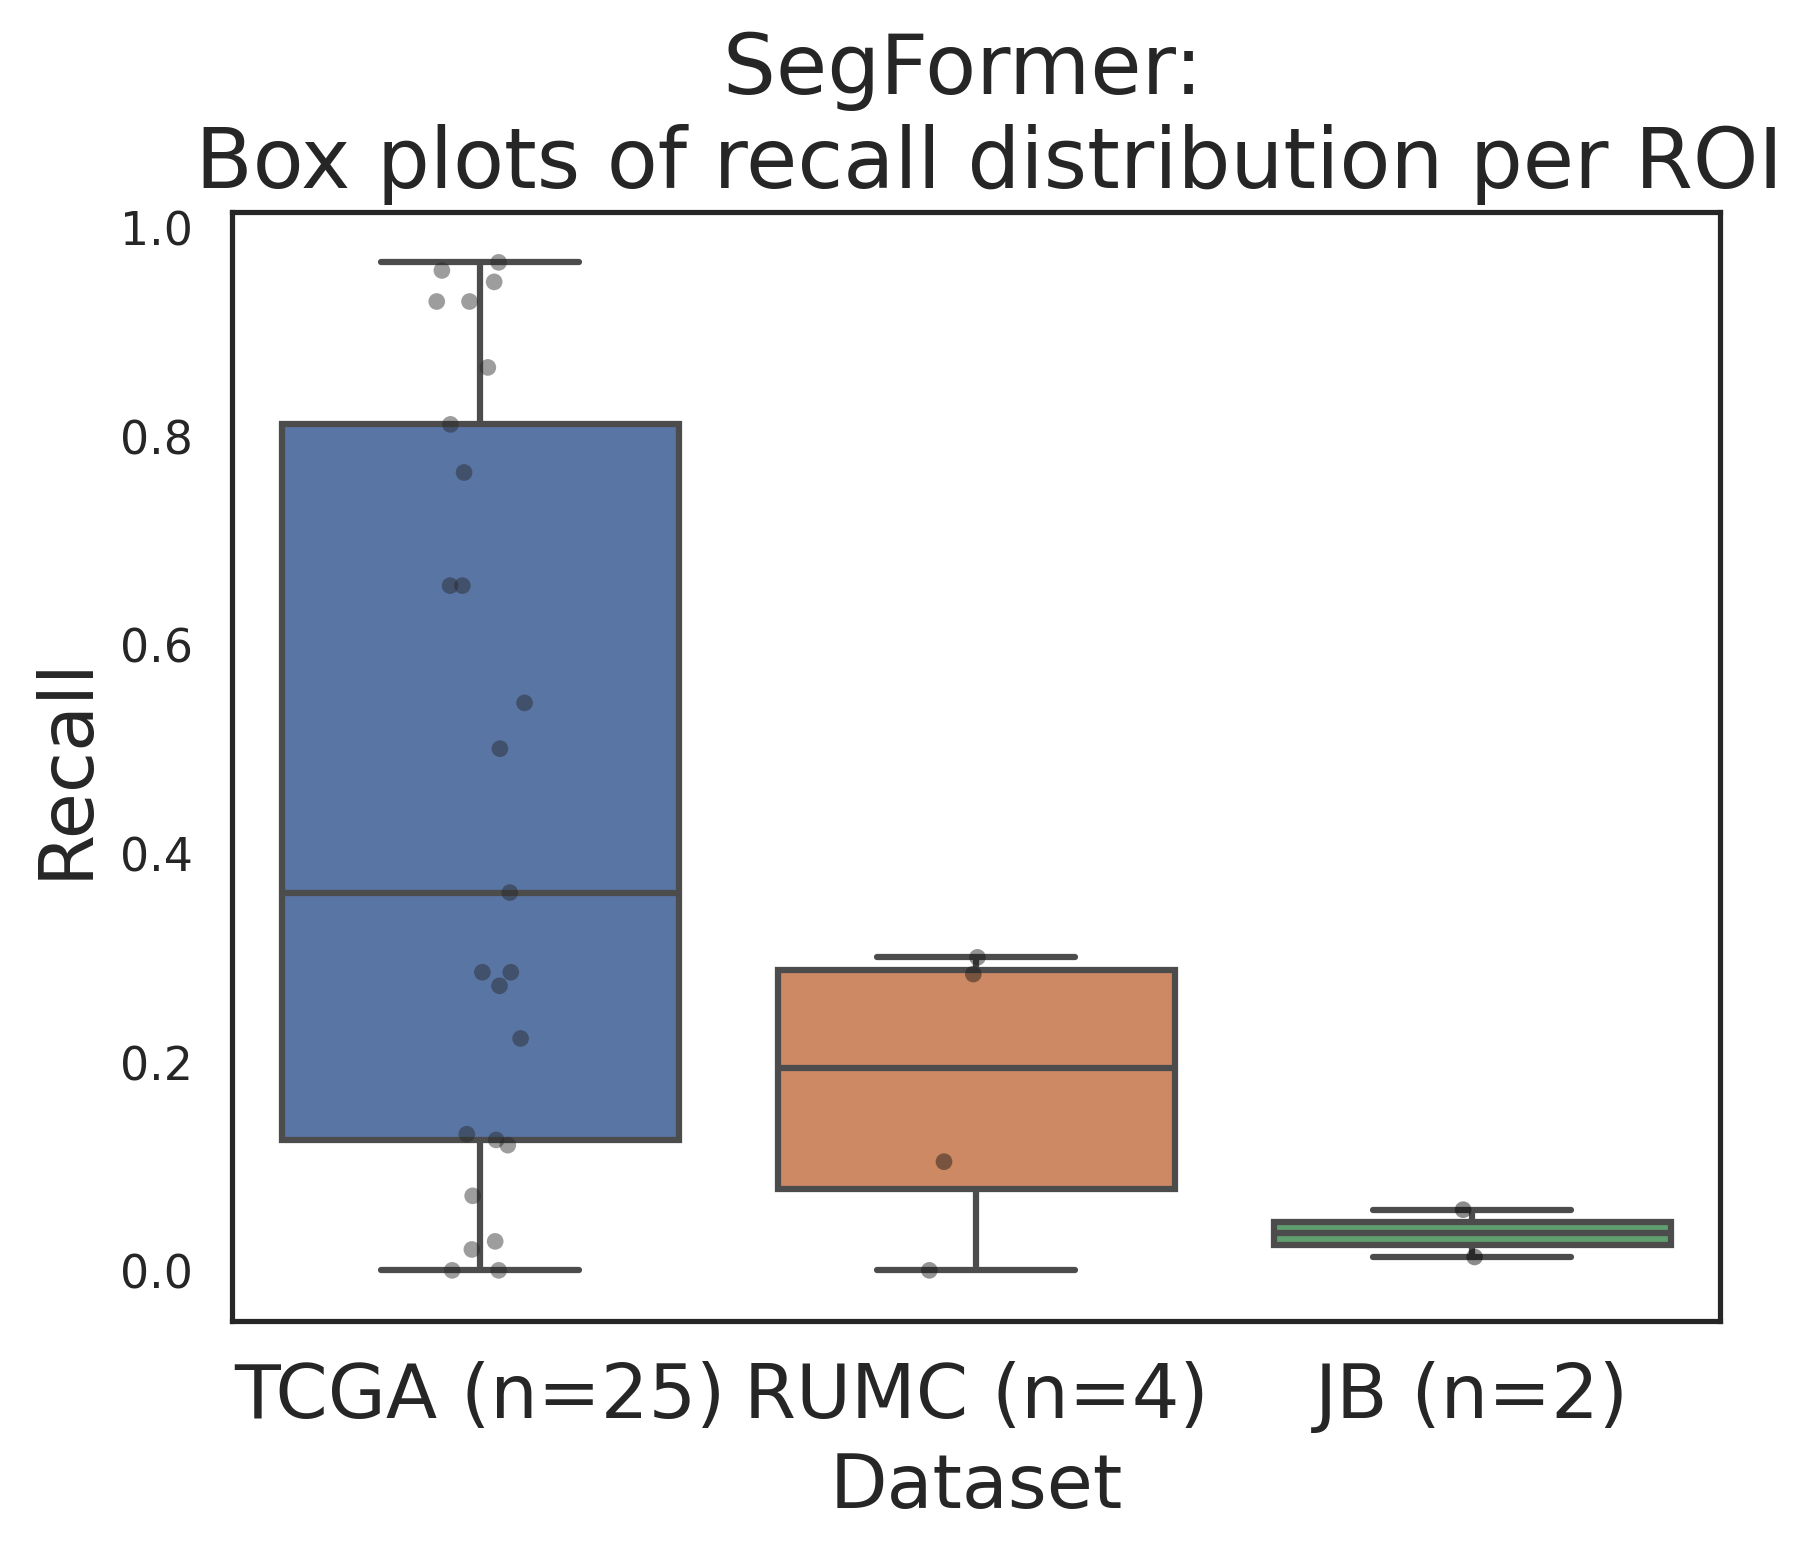
\includegraphics[width=.32\linewidth]{figures/tils/segformer_recall_roi_adj.png}
    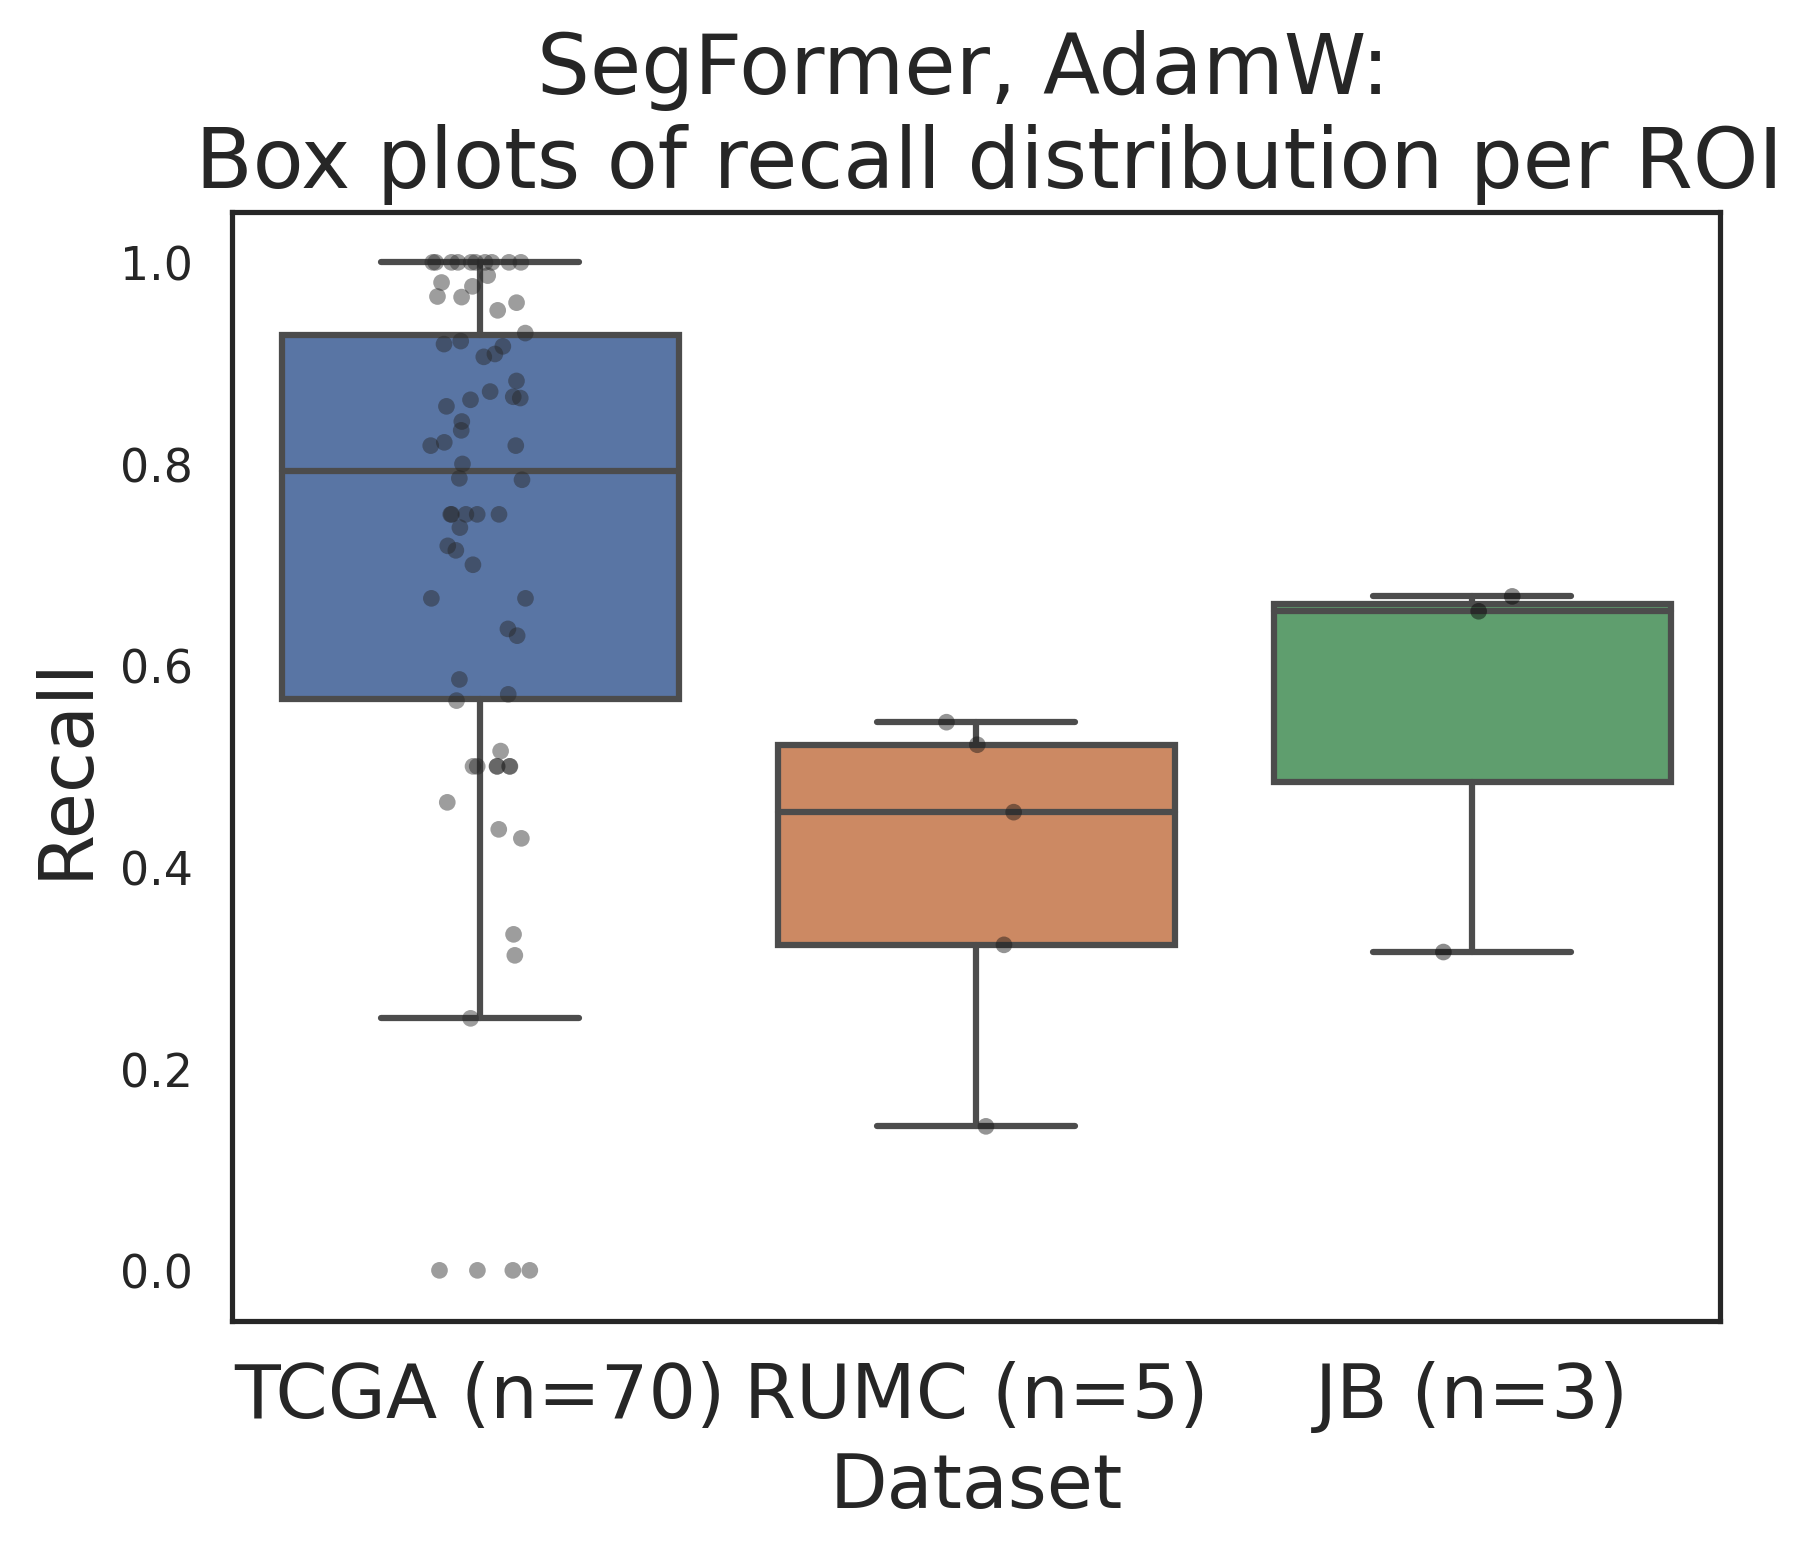
\includegraphics[width=.32\linewidth]{figures/tils/segformer,_adamw_recall_roi_adj.png}
    \caption{Boxplots of precision and recall across three datastes (TCGA-BRCA, RUMC, JB) with
    maximum allowed distance between ground truth and prediction equals 10 pixels (5 \textmu m).}
    \label{fig:tils_pr_r_boxplots}
\end{figure}

To evaluate the results of TILs detection TiGER challenge performed a
Free Response Operating Characteristic (FROC) analysis, computing sensitivity
versus average false positives per mm$^2$ over all test slides.
The experimental set included 26 WSIs and 38 WSIs in the final dataset.
The FROC ratio for three developed models was calculated on 173 test ROIs
since there was no possibility to submit the models to the server, nor access
the challenge's test data. The results can be viewed in Table~\ref{tab:tils_compare}.
The FROC analysis revealed huge differences between the trained model in the thesis.
Even though the values are not directly comparable, since they are based on different
data sets. SegFormer, AdamW yield a FROC value close to 0.7, which lies in a higher
range compared to TiGER results.
Both the experimental and final TiGER best models belong to the Bio-totem team.
They based the model on a modified SFCN-OPI network~\cite{zhou2018sfcn} which
is a sibling fully convolutional network that performs nuclei detection and
classification using weak labels.  The resulting SFCN-OPI first contains a
detection FCN branch, then the regions with high confidence of TILs
existence from detection output are gathered with thresholding (objectness prior)
and fed into the false positive suppressing branch for the TILs detection task. 

\begin{table}[H]
    \centering
    \begin{tabular}{ l c c c c c c }
        \hline
         & \multirow{2}{*}{DeepLabv3+} & \multirow{2}{*}{SegFormer} & SegFormer, & & TiGER best & TiGER best\\
         &  &  & AdamW & & (experimental) & (final)\\
        \hline
        FROC score & 0.432 & 0.326 & 0.693 & & 0.600 & 0.5504 \\
        \hline
    \end{tabular}
\caption{\label{tab:tils_compare} Free Response Operating Characteristic (FROC)
analysis for TILs detection. The TiGER challenge leaderboard results versus three
models developed in this work. The results were obtained from different data.}
\end{table}

Once again, just as for tissue segmentation AdamW optimizer for transformer
based method proved to be a better choice. 
But the statements that were done in the previous chapter~\ref{res_tissue_segm}
regarding tissue segmentation models comparison do not apply here, since SegFormer with AdamW
optimizer manages to outperform DeepLabv3+ even though no pre-training
or hyperparameter tuning was used. 
As Naseer, M et al.~\cite{naseer2021intriguing} discovered, when presented
with the texture and shape of the same object, in this case typically dark,
round to ovoid TIL, CNN models often make decisions based on texture. In contrast,
transformers perform better than CNNs on shape recognition. This indicates the
robustness of transformers to deal with significant distribution shifts and might
be the reason for superior performance, due to for instance better recognition of
TILs shapes in non-homogeneously stained slides. Taking into account all
discussions above and the overall better performance, the SegFromer AdamW was
considered the best model, and the model with the highest pixel-wise dice score
on the validation set was taken to the next step. 
For model inference, the model with the best pixel-wise Dice score on the validation set was used.
Patches of size 128$×\times$128 were extracted from the tissue region at 20$\times$ magnification
with a stride of 100. The whitespace was extracted by using thresholding and
inference of non-background pixels was then performed.

\begin{figure}[H]
    \centering
    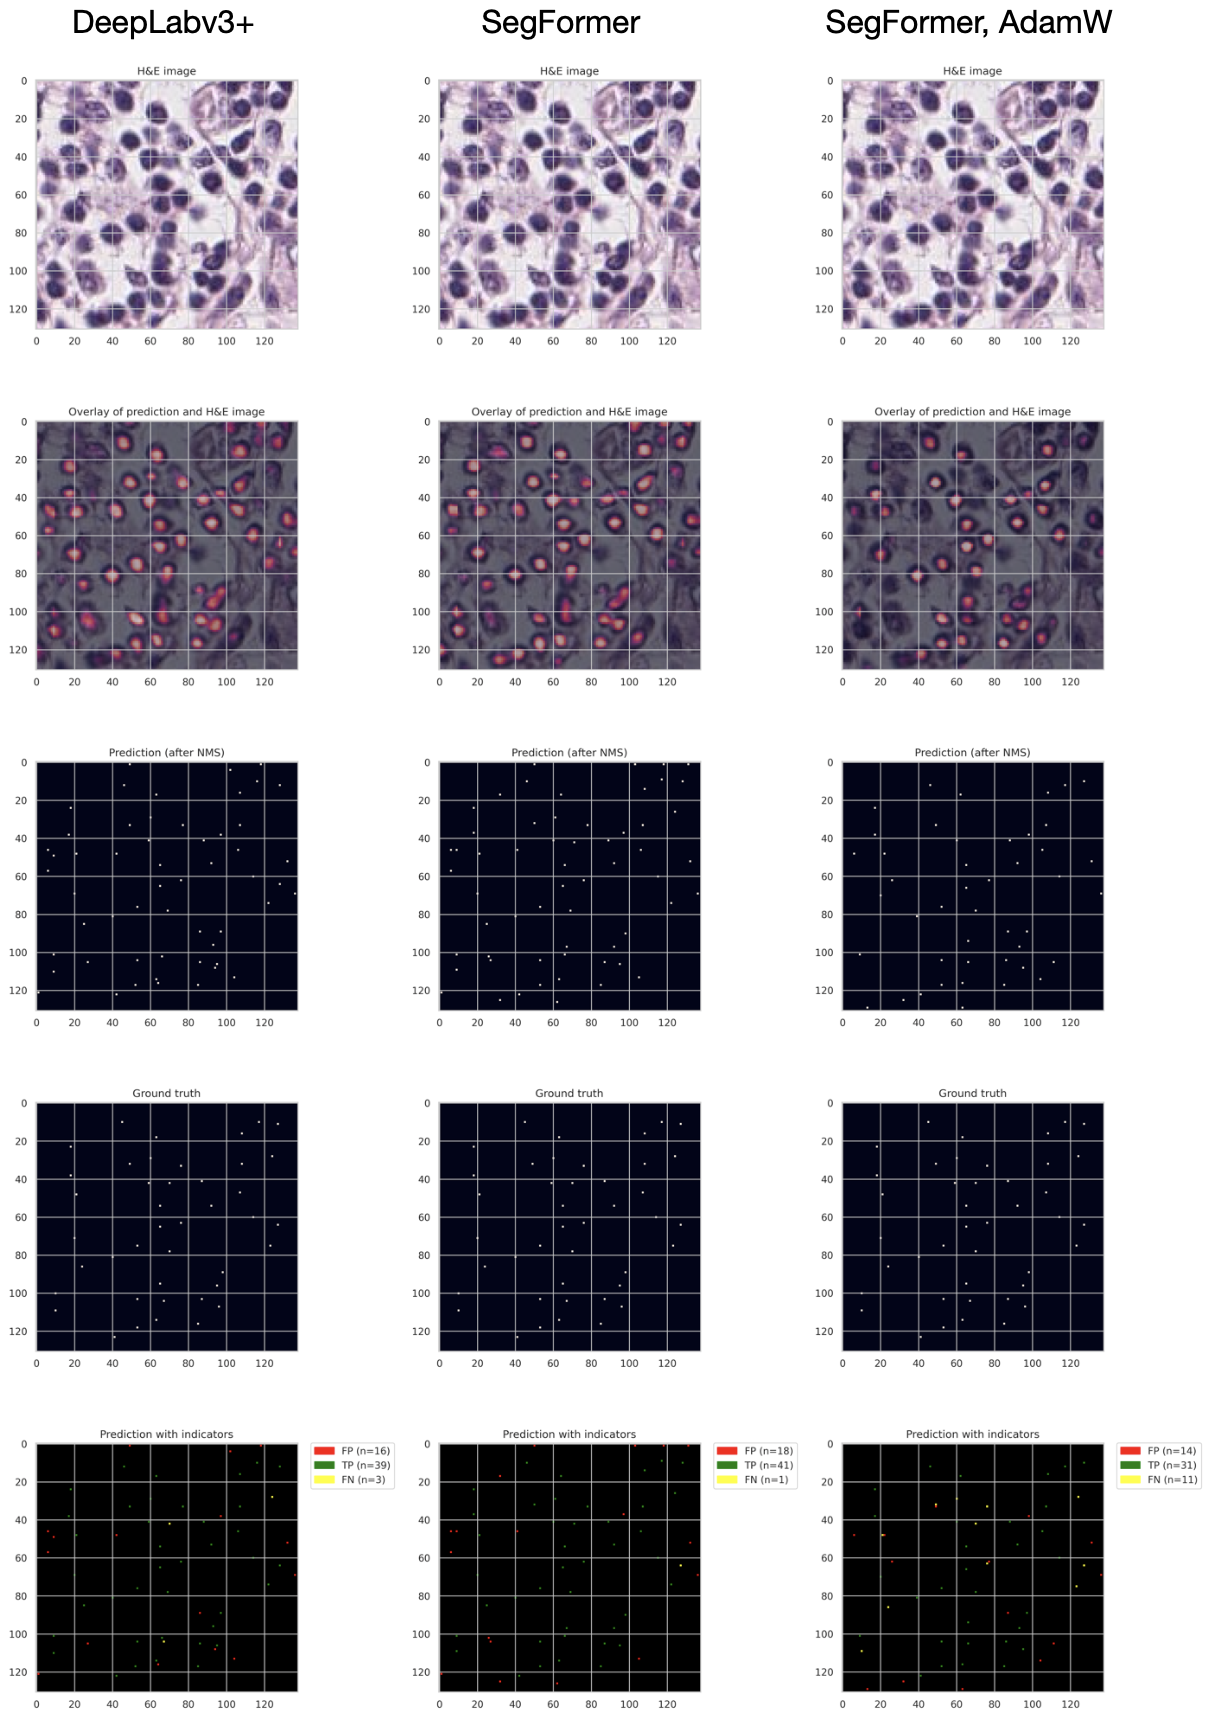
\includegraphics[width=0.95\textwidth]{figures/tils/TCGA-D8-A142-01Z-00-DX12.png}
    \caption{TCGA-D8-A142-01Z-00-DX12 TILs prediction with DeepLabv3+, SegFormer and
    SegFormer, AdamW. With 0.713, 0.804 and 0.812 F1 scores accordingly.}
    \label{fig:TCGA-D8-A142_tils}
\end{figure}

\section{Survival Analysis}
\todo[inline]{The following results are generated with DeepLabv3+ TILs detection. Missing heterogeneity features. Waiting for the results to generate. If everything goes wrong, those are the final results. Hopefully not.}
The patients from TCGA-BRCA clinical data with negative or not complete event times were removed. The remaining
1005 patients were used for survival analysis.
1133 segmented diagnostic slides were saved at 5$\times$ magnification. Each slide has determined regions of tumor, stroma,
and rest, as well as a list of all selected TILs. Based on this information four groups of TILs
densities were calculated: in stroma, stroma border, tumor associated stroma border,
and tumor border. The description of the regions is visualized in Figure~\ref*{fig:borders}.
The features for patients with multiple slides were mean aggregated.
\begin{wrapfigure}{r}{0.45\textwidth}
    \centering
    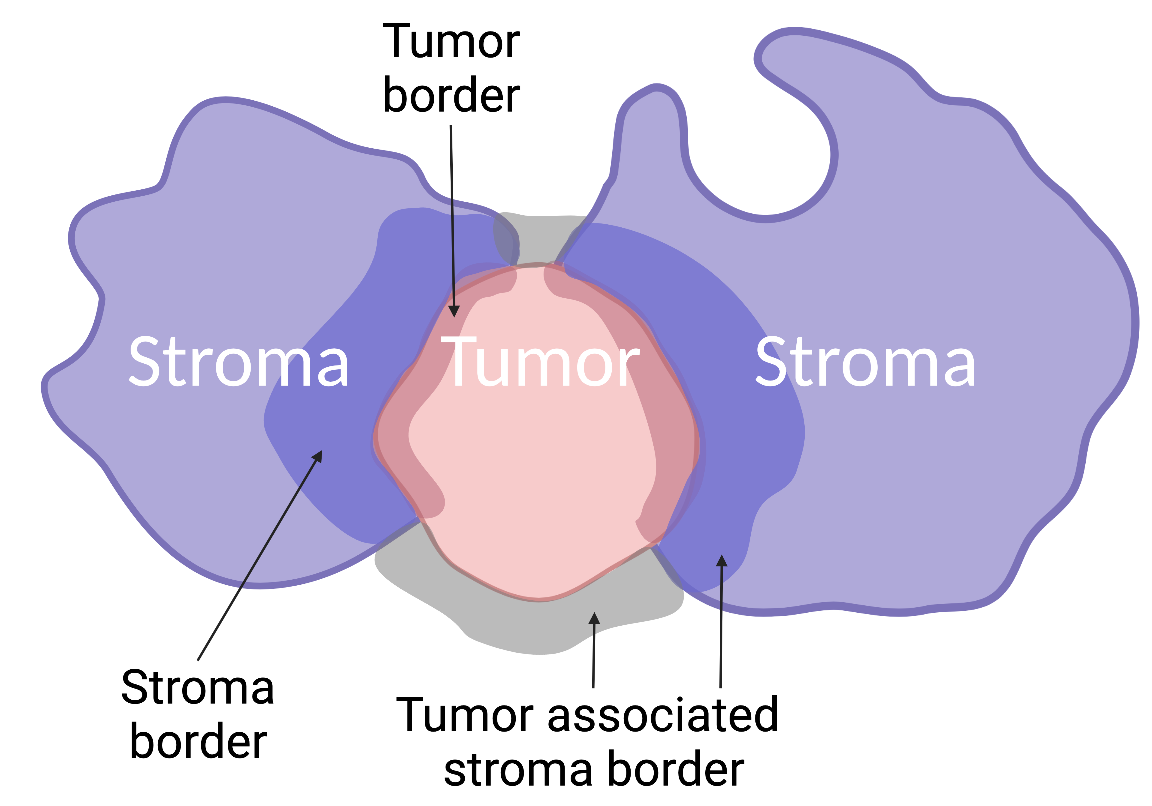
\includegraphics[width=0.45\textwidth]{figures/survival/tils_scheme.png} 
    \caption{Schematic border explanation. Created with BioRender.com}
    \label{fig:borders} 
\end{wrapfigure}
The overall TILs density in stroma was considered a baseline feature.
All densities were calculated as $\frac{\textrm{ Number of TILs}}{\textrm{Area in } mm^2}$.
For each border region, different widths were used. Tumor border experiments included
lower border widths of 10-40 \textmu m. Whereas stroma borders ranged between 50
and 350\textmu m.
Additionally, tumor associated stroma border of 125 \textmu m was included, since this is
the optimal border found for breast cancer patients~\cite{thagaard2021automated}.
It resulted in 20 features
that were first evaluated on correlation as depicted on a heatmap Figure~\ref{fig:heatmaps_tils}.
There are three coherent groups visible in Figure~\ref{fig:heatmaps_tils}.
There is a clear link between different groups and the baseline, such as a high correlation
of TILs density in stroma with TILs densities in stroma borders, which increases the bigger
the border gets. And on a contrary, a lower correlation of baseline with TILs density in tumor borders.
The values of pair-wise Pearson correlations in each group were compared and the columns with
a correlation higher than 90\% were removed. If all columns in a group displayed a
correlation above 90\%, the most similar column of a group was kept, which should
represent a group best. The resulting features and their correlations can be seen on the right heatmap
in Figure~\ref{fig:heatmaps_tils}.
\begin{figure}[h!]
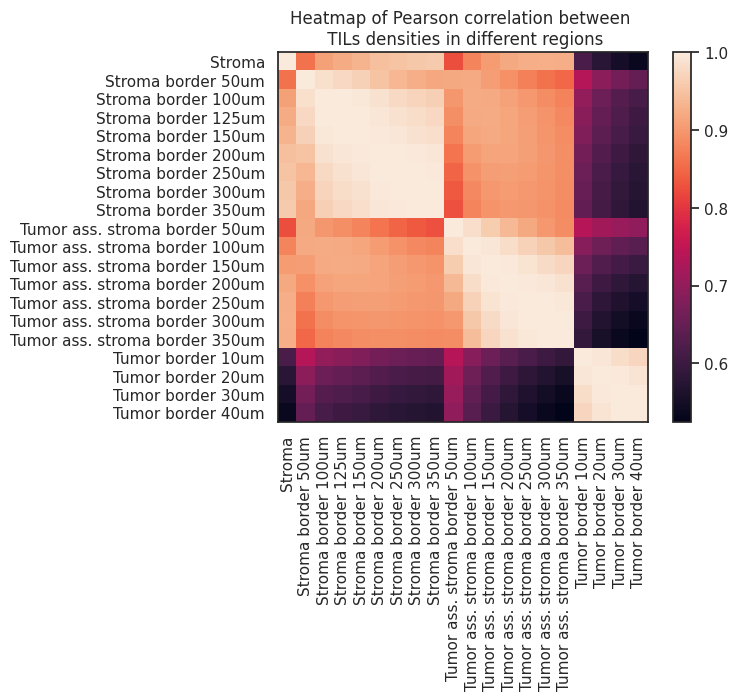
\includegraphics[width=.5\linewidth]{figures/survival/heatmap_tils.png}
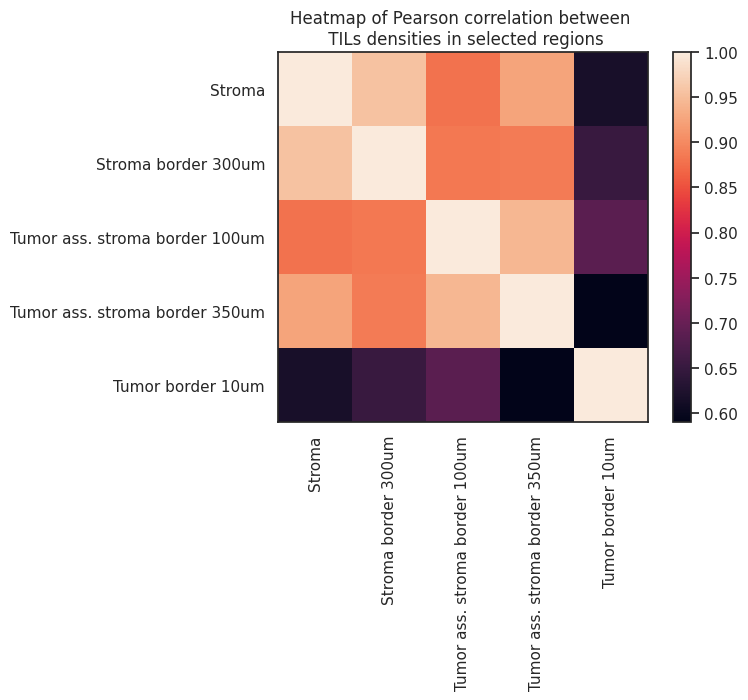
\includegraphics[width=.5\linewidth]{figures/survival/heatmap_tils_min.png}
\caption{Heatmaps representing pair-wise Pearson correlation between TILs densities in different areas.
Full version and condensed to group representatives.}
\label{fig:heatmaps_tils}
\end{figure}
For further comparison, features were evaluated at different prevalences.
For every feature, the patients were sorted descending according to a current feature.
For every prevalence in the range of 0.2 until 0.9, the patients were separated into
according groups and the Kaplan Meier method was used on both of them. The Log-Rank test
was applied to measure whether the two resulting event series are statistically different.
The resulting p-values are visualized in Figure~\ref{fig:pvalues_tils}, both as a line plot
per each prevalence, as well as a boxplot. In the boxplot, it can be seen that the median
p-value of the density in 100 \textmu m tumor associated stroma and in 10 \textmu m tumor
border lay higher than the other features. Those densities are also found more frequently
over the statistical significance line in the line plot. Those features were decided to exclude.
And for visibility, the remaining features were plotted again separately in
Figure~\ref{fig:pvalues_tils_selected} with an additional boxplot depicting differences in median
survival time at the same prevalence range. TILs density in tumor associated stroma achieving
lower p-values in the lower prevalences. But TILs density in stroma border shows a better
performance overall. It is also a feature that stays under the significance line across
all prevalences. Additionally, according to the Median survival time boxplot,
the median value of TILs densities in stroma border is 1.5 years higher.

For fitting the data into a Cox model, the TILs densities were divided by 100.
The result revealed 0.58 concordance, 0.01 p-value, and 0.94 hazard ratio.
That means that the coefficient is negative (-0.06) which supports the assumption
that the high level of TILs plays a role in longer survival probability.
For the TILs density in stroma border, the result is identical: 0.58 concordance,
0.01 p-value, and 0.94 hazard ratio. And TILs density in tumor associated stroma
reaches 0.59 concordance, 0.01 p-value, and 0.88 hazard ratio.
Regression models generally give more reliable results with normally-distributed variables.
Since the TILs densities are not normally-distributed (see Figure~\ref{fig:histo_tils}),
the experiments were repeated with log features. The TILs densities in stroma scored
0.58 concordance, p-value 0.00064 and 0.8 hazard ratio, for TILs desnities in stroma border - 0.58
concordance, p-value 0.00034 and 0.79 hazard ratio, and TILs densities in tumor
associated stroma - concordance of 0.59, p-value 0.00019 and 0.78 hazard ratio.
It was expected for concordance to stay indifferent since it was not influenced by
taking the log of all values. Whereas p-values and hazard ratios improved drastically.
It is harder to explain the signal presence and meaning of log-ed features,
hence we will concentrate on raw values.

\begin{figure}[H]
\centering
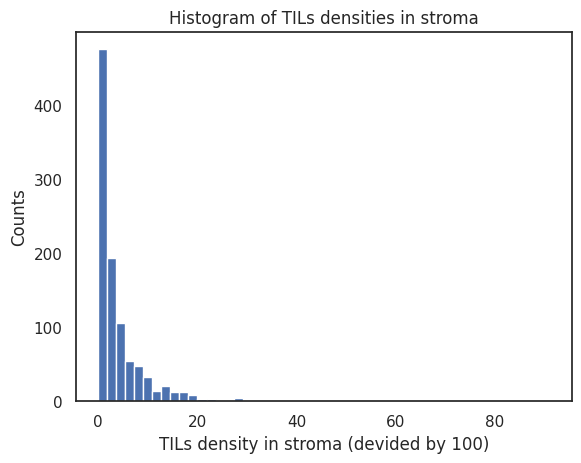
\includegraphics[width=0.4\linewidth]{figures/survival/histo_tils.png}
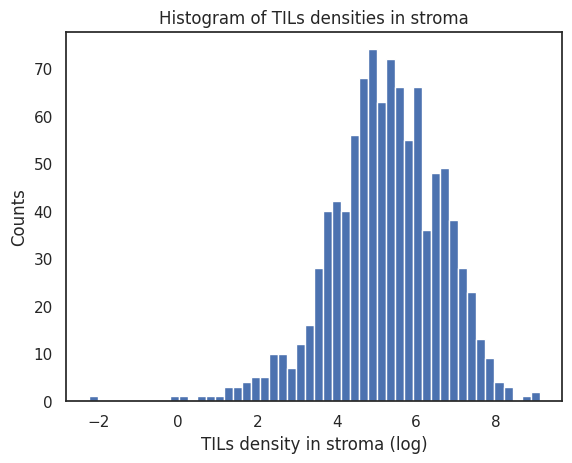
\includegraphics[width=0.4\linewidth]{figures/survival/histo_tils_log.png}
\caption{Histograms of baseline TILs density in stroma features versus its log distribution.}
\label{fig:histo_tils}
\end{figure}
    

The Kaplan Meier curves in Figure~\ref{fig:km} at most often viewed prevalences of
0.33, 0.66, and the median matched the cases when TILs density in tumor associated
stroma features stratified patients better in lower range and median.
Whereas at 0.66 the TILs density in stroma border scores a slightly more significant p-value.
The observation that a border of stroma or tumor associated stroma features perform better
than the stroma itself may come from the observed behavior that the tissue segmentation model
leans to confuse rest with stroma (Figure~\ref{fig:tissue_confusion}).
Hence, taking into consideration only regions close to tumorous regions, that are better
segmented, acts as a filtering of falsely annotated regions that therefore leads to a higher
significance of a feature.

\todo[inline]{When the final results are done, here same analysis of Her2+, TNBC subsets.}

\begin{figure}[h!]
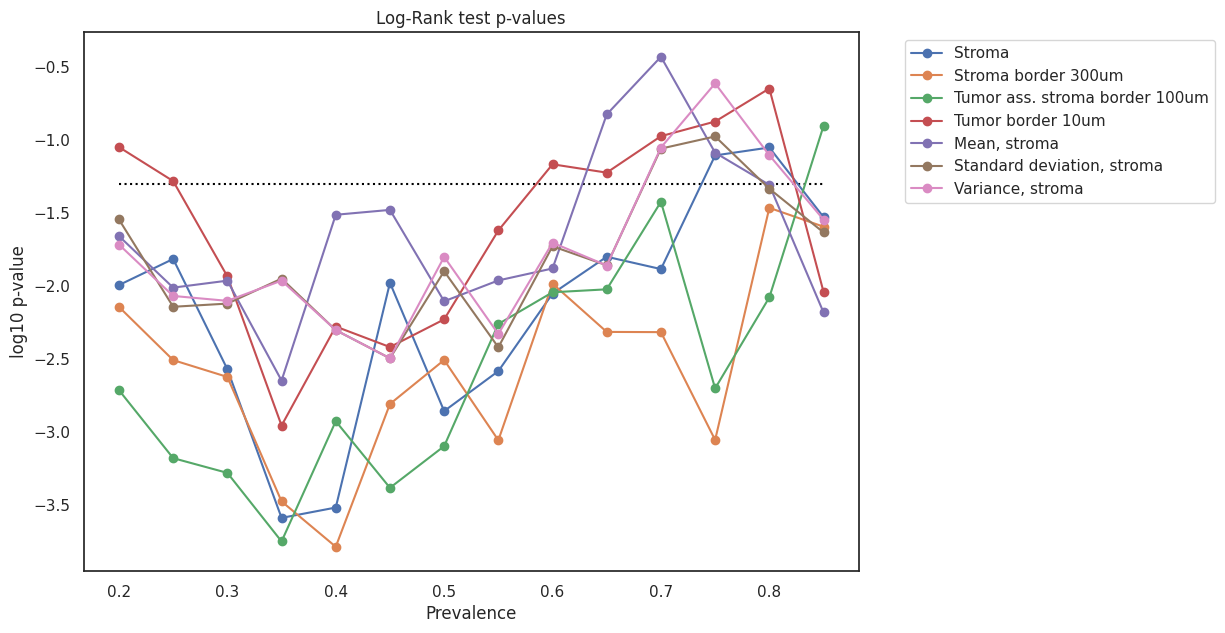
\includegraphics[width=\linewidth]{figures/survival/pvalue_prevalence_all.png}
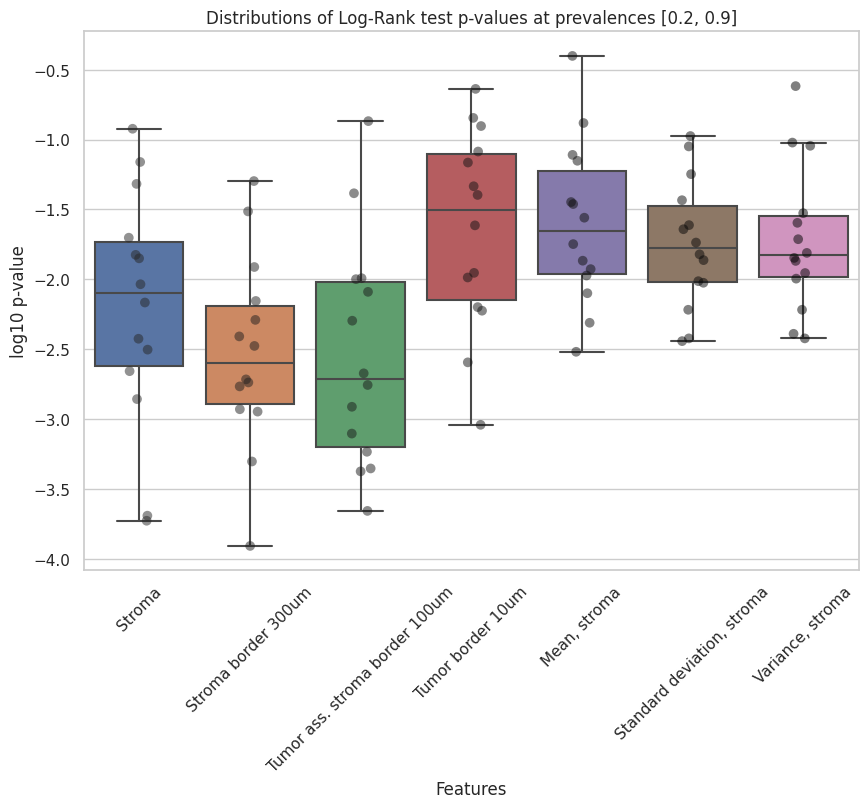
\includegraphics[width=0.764\linewidth]{figures/survival/pvalue_boxplot_all.png}
\caption{Log-Rank p-values distribution by different patient separations.
The dotted line in the line plot represents the significance level of 0.05 ($\log_{10} 0.05$)}
\label{fig:pvalues_tils}
\end{figure}

\begin{figure}[h!]
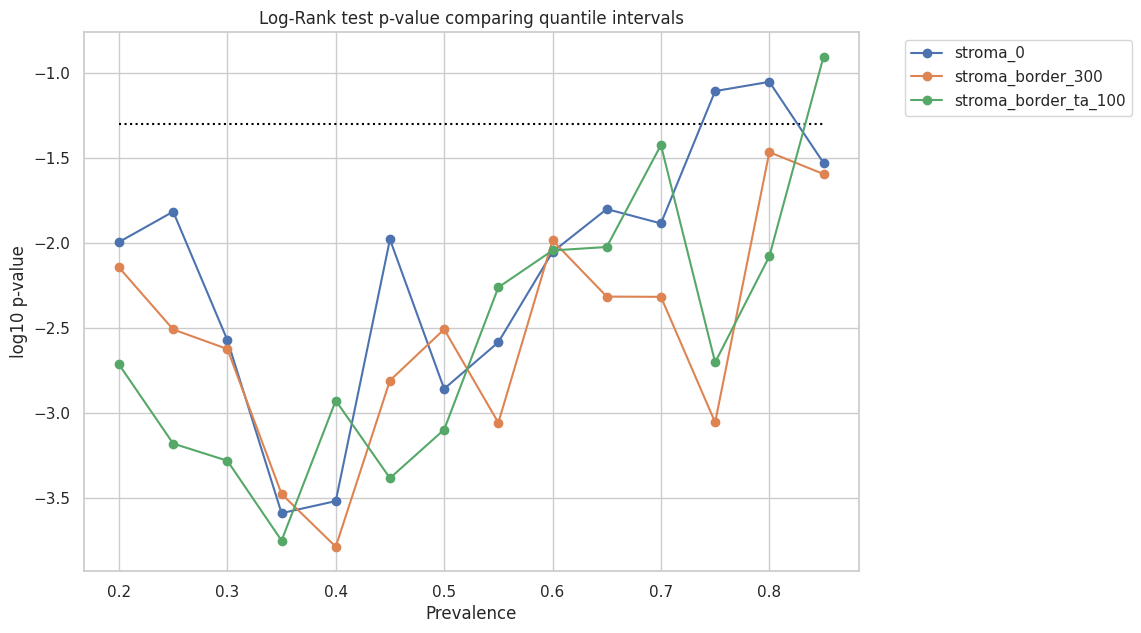
\includegraphics[width=\linewidth]{figures/survival/pvalue_prevalence_selected.png}
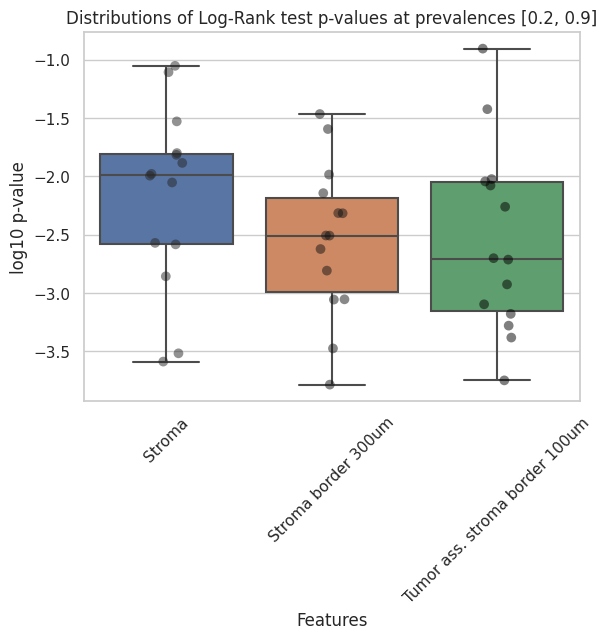
\includegraphics[width=0.5\linewidth]{figures/survival/pvalue_boxplot_selected.png}
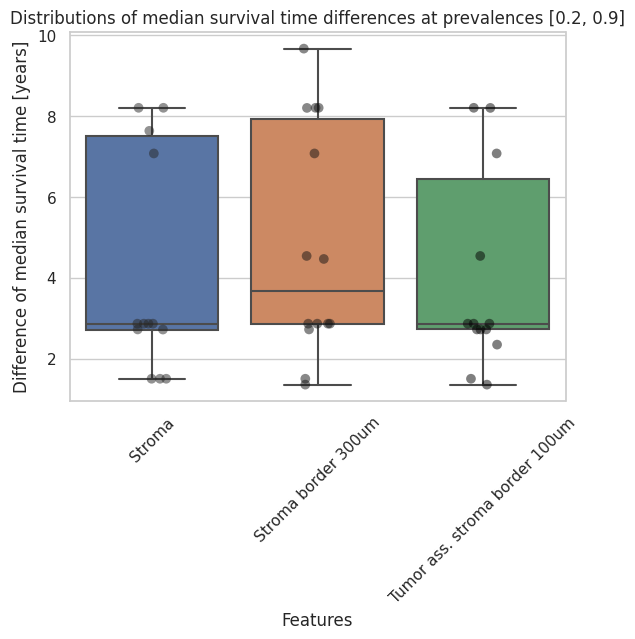
\includegraphics[width=0.5\linewidth]{figures/survival/surv_time_boxplot_selected.png}
\caption{Log-Rank p-values distribution by different patient separations with an additional boxplot
with median survival time differences. The dotted line in the line plot represents the significance level of 0.05 ($\log_{10} 0.05$)}
\label{fig:pvalues_tils_selected}
\end{figure}

\begin{figure}[h!]
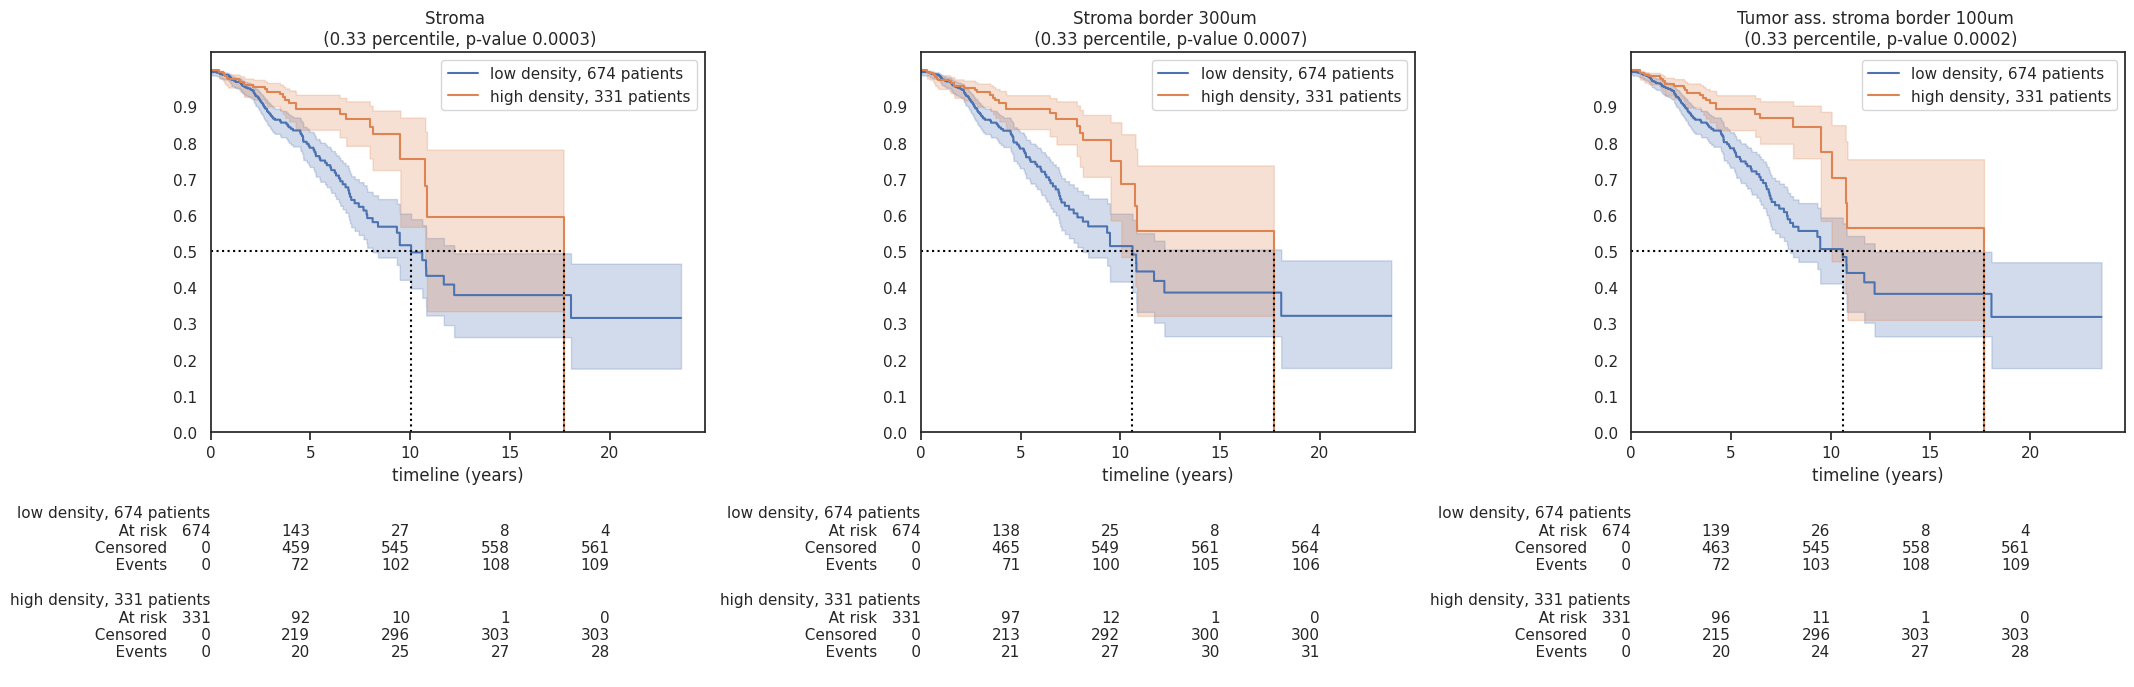
\includegraphics[width=\linewidth]{figures/survival/km_33.png}
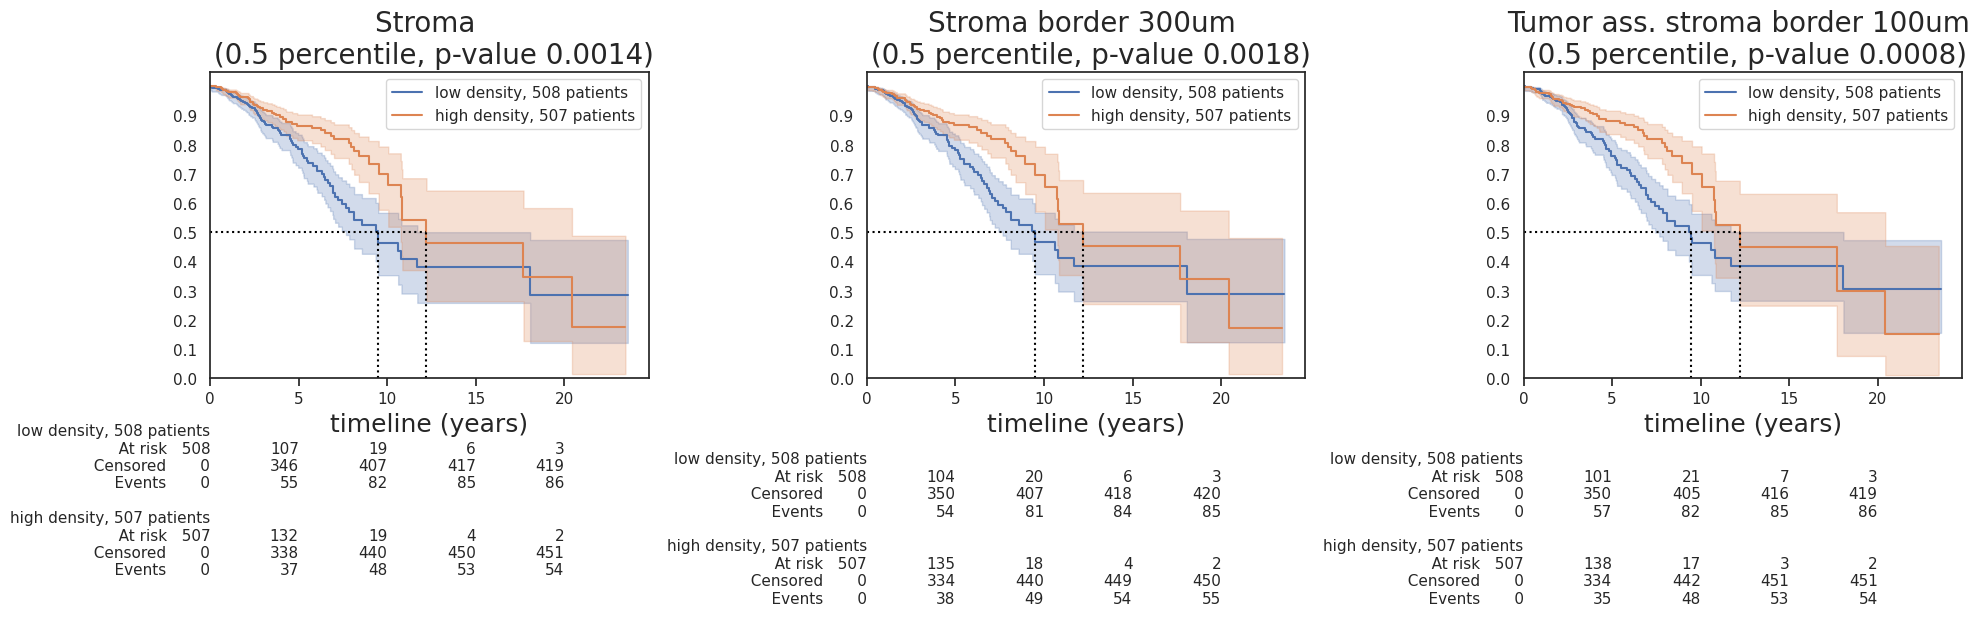
\includegraphics[width=\linewidth]{figures/survival/km_50.png}
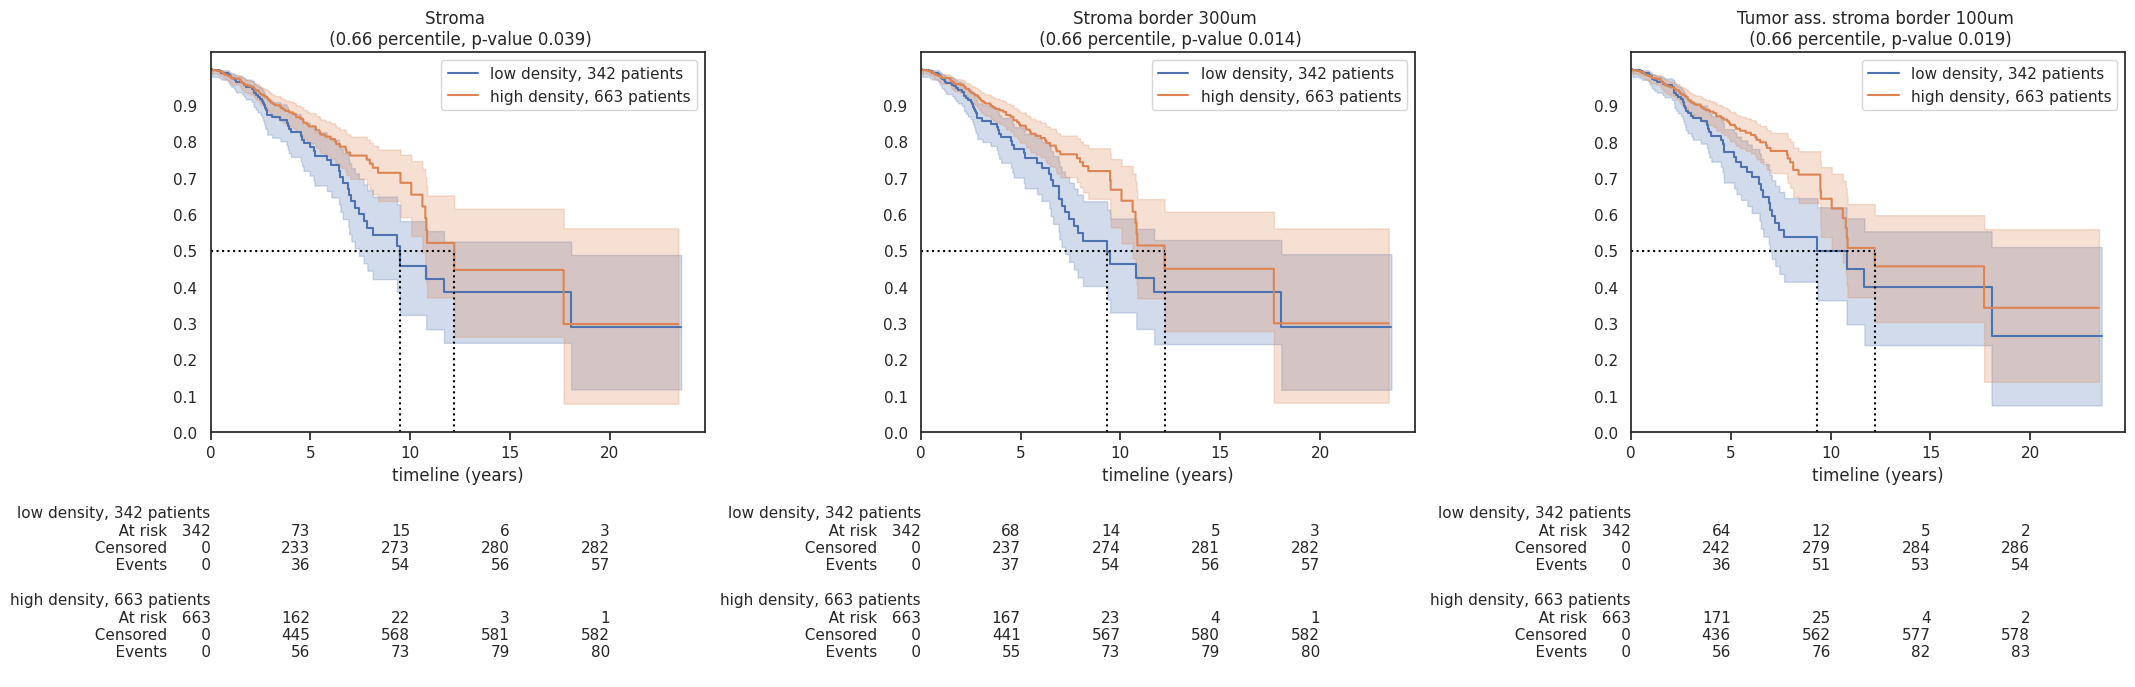
\includegraphics[width=\linewidth]{figures/survival/km_66.png}
\caption{Kaplan Meier curves. Columns correspond to denisty features in: stroma, 300 \textmu m stroma border,
100 \textmu m tumor associated stroma border. Rows coorespond to following prevalences: 0.33, 0.5, and 0.66.}
\label{fig:km}
\end{figure}

%\begin{figure}[h!]
%\includegraphics[width=0.5\linewidth]{figures/survival/boxplot_sep.png}
%\caption{Value separation}
%\label{fig:v_sep}
%\end{figure}